\documentclass[english, a4paper, 12pt, twoside]{book}

% -------------- Setup, do not change these ---------------
\usepackage{textcomp}
\usepackage[T1]{fontenc, url}
\usepackage[utf8]{inputenc}
\usepackage{titlesec}
\setcounter{secnumdepth}{4}
\usepackage{multirow}
\usepackage{braket}

\usepackage{adjustbox}
\usepackage{graphicx}
\usepackage{wrapfig}
\usepackage{amsmath, amssymb, amsthm} % Mathematical packages
\usepackage{parskip} % Removing indenting in new paragraphs
\urlstyle{sf}
\usepackage{color}
\usepackage{subcaption}
\usepackage{appendix}
\usepackage{chngcntr} % needed for correct table numbering
\counterwithin{table}{section} % numbering of tables
\counterwithin{figure}{section} % numbering of figures
\numberwithin{equation}{section} % numbering of equations
\hyphenpenalty=100000 % preventing splitting of words
\sloppy
\raggedbottom
\usepackage{xparse,nameref}
\usepackage[bottom]{footmisc} % Fotnotes are fixed to bottom of page


% --------- You can edit from this point on --------


% ----- Appearance and language -----
\usepackage[english]{babel} % document language
\graphicspath{{./img/}} % path to images
\usepackage[margin=2.54cm]{geometry} % sets margins for the document
\usepackage{setspace}
\linespread{1} % line spread for the document
\usepackage{microtype}
\usepackage{pdfpages}

% ----- Sections -----
\titleformat*{\section}{\LARGE\bfseries} % \section heading
\titleformat*{\subsection}{\Large\bfseries} % \subsection heading
\titleformat*{\subsubsection}{\large\bfseries} % \subsubsection heading
% next three lines creates the \paragraph command with correct heading
\titleformat{\paragraph}
{\normalfont\normalsize\bfseries}{\theparagraph}{1em}{}
\titlespacing*{\paragraph}
{0pt}{3.25ex plus 1ex minus .2ex}{1.5ex plus .2ex}


% ----- Figures and tables -----
\usepackage{fancyhdr}
\usepackage{subfiles}
\usepackage{array}
\usepackage[rightcaption]{sidecap}
\usepackage{wrapfig}
\usepackage{float}
\usepackage[labelfont=bf]{caption} % bold text for captions
\usepackage[para]{threeparttable} % fancy tables, check these before you use them
\usepackage{url}
\usepackage[table,xcdraw]{xcolor}
\usepackage{makecell}
\usepackage{hhline}
\usepackage{booktabs}

\usepackage[breaklinks=true,colorlinks=true,linkcolor=black,urlcolor=blue,citecolor=blue]{hyperref}
% ----- Sources -----


%\bibliographystyle{apa} % citation and reference list style
%\def\biblio{\clearpage\bibliographystyle{apa}\bibliography{References.bib}} % defines the \biblio command used for referencing in subfiles - DO NOT CHANGE


% ----- Header and footer -----
\pagestyle{fancy}
\fancyhead[RO,LE]{\thepage} % page number on right for odd pages and left for even pages in the header
\fancyhead[RE,LO]{\nouppercase{\rightmark}} % chapter name and number on the right for even pages and left for odd pages in the header
%\renewcommand{\headrulewidth}{0pt} % sets thickness of header line
\fancyfoot{} % removes page number on bottom of page
\usepackage{emptypage}

% ----- Header of the frontpage -----
\fancypagestyle{frontpage}{
	\fancyhf{}
	\renewcommand{\headrulewidth}{0pt}
	\renewcommand{\footrulewidth}{0pt}
	\vspace*{1\baselineskip}

	%\fancyhead[R]{Norwegian School of Economics
	%\linebreak       Bergen, Fall 2018\vspace*{5\baselineskip}}
	\fancyhead[C]{ 
\includegraphics[width=3.5in]{img/logo}}
}


% ----- Document starts here -----
\begin{document}

%\def\biblio{} % resets the biblio command, if not here a new reference list will be produced after every chapter
{\setstretch{1.5}

\begin{titlepage}

 \newgeometry{top=1 in, bottom=1 in, left=1 in, right= 1 in}

 \thispagestyle{frontpage}

 \begin{center}

   \vspace*{6\baselineskip}


   {\Huge \textbf{Fancy title with many fancy words\\}}

   

       \vspace*{1,5\baselineskip}


   \vspace{1,5\baselineskip}

   \large{A master’s thesis submitted to the faculty of mathematics, computer science and physics, of the University of Innsbruck\\ in partial fulfillment of the requirements for the degree of\\\vspace{1,2\baselineskip}\textbf{Master of Science (MSc)} \\\vspace{1,2\baselineskip}carried out at the Institute of Experimental Physics under the supervision of}\\
   \large{o.Univ.-Prof.  Dr.  Rainer Blatt,}\\
   \large{Dr. Ben Lanyon}\\
    \vspace{1,2\baselineskip}
   \large{Presented by\\}
   \huge{\textbf{Marco Canteri}}\\
   

 \end{center}

\end{titlepage}

}
\restoregeometry % restores the margins after frontpage
%\nocite{*} % uncomment if you want all sources to be printed in the reference list, including the ones which are not cited in the text

\pagenumbering{gobble} % suppress page numbering
\thispagestyle{plain} % suppress header
\clearpage\mbox{}\clearpage % add blank page

\pagenumbering{roman} % starting roman page numbering
\newpage

\section*{Abstract}
An ongoing project of building a three node quantum network is currently carried out at the university of Innsbruck with ion traps being the nodes of the network. To make entanglement between ions located in the three nodes, control over multiple ion-photon pairs is required. A laser beam has to focused down to a single ion to generate photons out of individual ions in a string. In this thesis, an optical system is designed and built for focusing and steering the laser beam responsible for the photon generation process. Our experiment traps $^{40}\text{Ca}^+$ ions, the 393 nm laser triggers the generation of a photon via a cavity enhanced Raman process. The photon is emitted in a cavity and leaks out from one side.
The designed setup comprises of an AOD, for steering the beam in the microsecond timescale, a set of lenses for expansion and control of the laser beam, and a custom objective for focusing the light on the ions. The system was designed and simulated with the software Zemax, and ultimately built on top of the existing experiment. We report two experiments that demonstrate the capabilities of the newly built setup. The first experiment generated photons out of a single ion in a string without exciting the ions not involved in the process. In the second experiment we applied a phase gate on a single ion-qubit, the phase shift induced is measured with a Ramsey interferometer. In addition to demonstrate single qubit manipulation capability, this experiment also allowed for a measure of the focus spot: 1.2-1.3 $\mu$m with an upper bound on the addressing error of $10^{-3}$. These experiments are a stepping stone towards the realization of the aforementioned quantum network, the next key experiment is already ongoing, photons are produced from different ions creating a photon train. Afterwards, entanglement between ion and photon has to be achieved for each ion-photon pair.
\newpage

\newpage
\tableofcontents


\newpage
\addtocontents{toc}{\protect\setcounter{tocdepth}{4}} % sets depth of toc to 4, 1.1.1.1
\pagenumbering{arabic} % Starting arabic page numbering
\setcounter{page}{1} % sets pagecounter to 1

\chapter{Introduction} % section/chapter name
A next step in technology advancement is represented by quantum technology, as it offers a radically new approach for the fields of computation, communication, simulation, and metrology \cite{quantumtech}. For example, classical computers are limited in solving some particular problems that scale exponentially, and therefore a new approach is needed. Quantum computing can exploit particular features of quantum mechanics that have no classical counterparts, this allows for a speed up for a certain class of problems such as factorizing numbers \cite{shor}, or searching in a database \cite{grover}. Moreover, simulating nature at its quantum level is a hard task for classical computer, while quantum computers are naturally prone to simulate quantum dynamics \cite{RevModPhys.86.153}.\\
A collection of quantum computers interconnected via quantum channels forms a fully fledged quantum network \cite{kimble}. However, for some quantum network applications, it is possible to relax the condition of having a universal quantum computer, a quantum device with a single qubit is enough as part of a functional quantum network with basic capabilities \cite{Wehnereaam9288}. The concept of a quantum internet is to have a quantum channel along side with the classical channel, enabling the transmission of quantum information \cite{Wehnereaam9288}. There are fundamental differences between a quantum channel and a classical link. Although the medium can be the same, such as optical fiber, a quantum channel must have additional abilities, such as distributing entanglement, or transmitting quantum states. Quantum networks have several applications: cryptographic wise they allow for more secure information transmission through Quantum Key Distribution \cite{qkd2}, secure identification \cite{secureident}, blind quantum computation \cite{blindcomputation} and more \cite{Wehnereaam9288}. Outside cryptography, quantum networks find applications in metrology: entanglement can be exploited to improve clock synchronization \cite{quantumclocks},
and extend telescope's baselines \cite{telescope}. Furthermore, quantum networks offer more efficient solutions to distributed system problems \cite{distributedcomputing}.\\
It is in this context that this thesis arises. Currently there is an ongoing project of building a three node quantum network between two buildings on the campus of the University of Innsbruck. The quantum nodes consist of ion traps: qubits are encoded in the electronic states of ions trapped in a Paul trap, while manipulation is done with laser pulses \cite{ionquantumcomputer}. A 400 m optical fiber serves as link between the two buildings. This quantum network should have the ability to make entanglement with more than one other node in a network. This task requires the ability to connect multiple ions to multiple traveling direction-switchable photons. This is achieved with a single-ion-focused laser beam.\\ % In this thesis, an optical system was designed and built for controlling and focusing the laser beam responsible for photon generation.\\
Photons are generated via a cavity enhanced Raman process \cite{stuteinterface}, for which a 393 nm laser is used. When I started my master project, the 393 nm laser was shining on every ion in the trap. In this case, if an ion string were to be loaded, the light would couple to every ion and there would be no control over the single ion-photon pair. The same 393 nm laser is also employed to perform ion-qubit manipulation by inducing an AC Stark shift on the qubit's ground state. A single-ion-focused laser allows to manipulate individual ion-qubits performing thus single qubit operations.\\
% To get photons from individual ions in a string,
This thesis presents the development of an optical system that focuses the 393 nm laser beam on a single ion, and has the ability to steer the beam on a timescale of a few microseconds, which is the typical time for photon generation operations and ion-qubit operations. The setup is per se not complex, but the design is critical. Ions separation is typically around 5 micrometers in our system, so the light should be focused down to $1-2\,\mu$m, at the limits of the optical elements involved. The steering part is achieved with an acousto-optical deflector (AOD), which deflects the laser light on microsecond timescales proportionally to the applied input frequency allowing to control remotely the beam pointing of the system.
The AOD allows single ions in a string to be manipulated in two different ways:\textcolor{white}{The AOD allows single ions in a string to be manipulated
 }\vspace{-.5em}
\hspace{3em}{\large\textbf{\textsc{Single ion photon generation}}}\\
\begin{wrapfigure}{l}{0.5\textwidth}
  \centering
    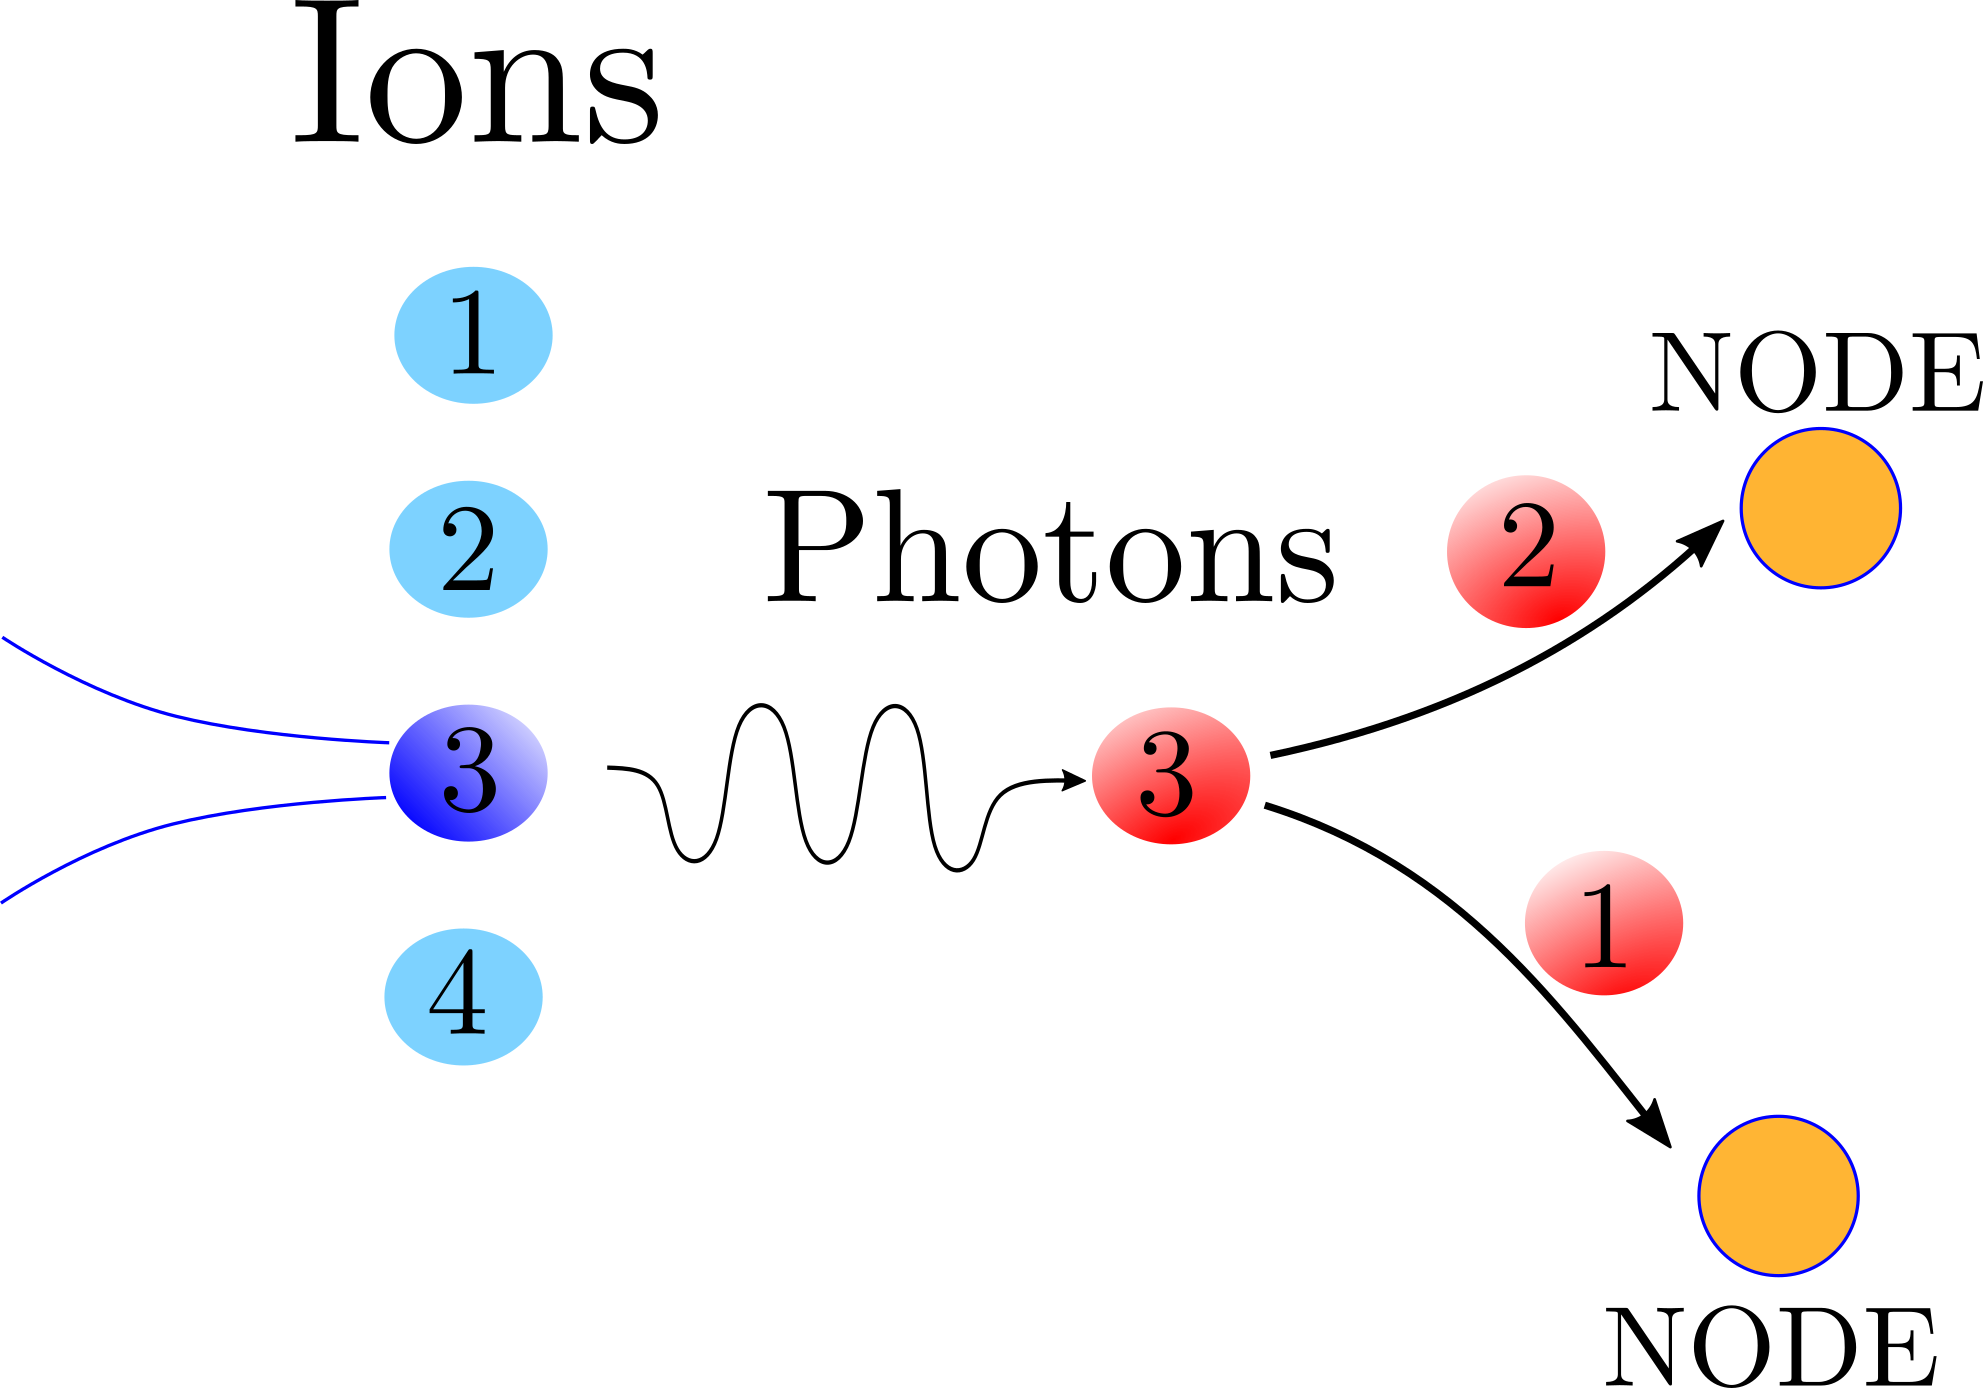
\includegraphics[width=0.48\textwidth]{photongeneration3}
  %\caption{Schematic of photon generation}
\end{wrapfigure}
As illustrated in the sketch on the left, the idea is to generate photons from individual ions in a string and send them to the different nodes of the network. The laser beam is focused on a single ion, a laser pulse triggers the generation of a photon, the beam is then steered and focused on another ion to repeat the process. The approach we use is an ion-cavity system: the laser pulse triggers a cavity enhanced Raman process \cite{stuteinterface} that on resonance causes the emission of a photon from one ion into the cavity. The photon subsequently leaks out from one of the cavity mirrors. In this thesis we set the goal of emitting photons from a particular ion without exciting any other ion in the string. This is a key step towards producing and controlling multiple photon-ion pairs.

\hspace{9em}{\large\textbf{\textsc{Single ion-qubit manipulation}}}\\

\begin{wrapfigure}{r}{0.4\textwidth}
\centering
    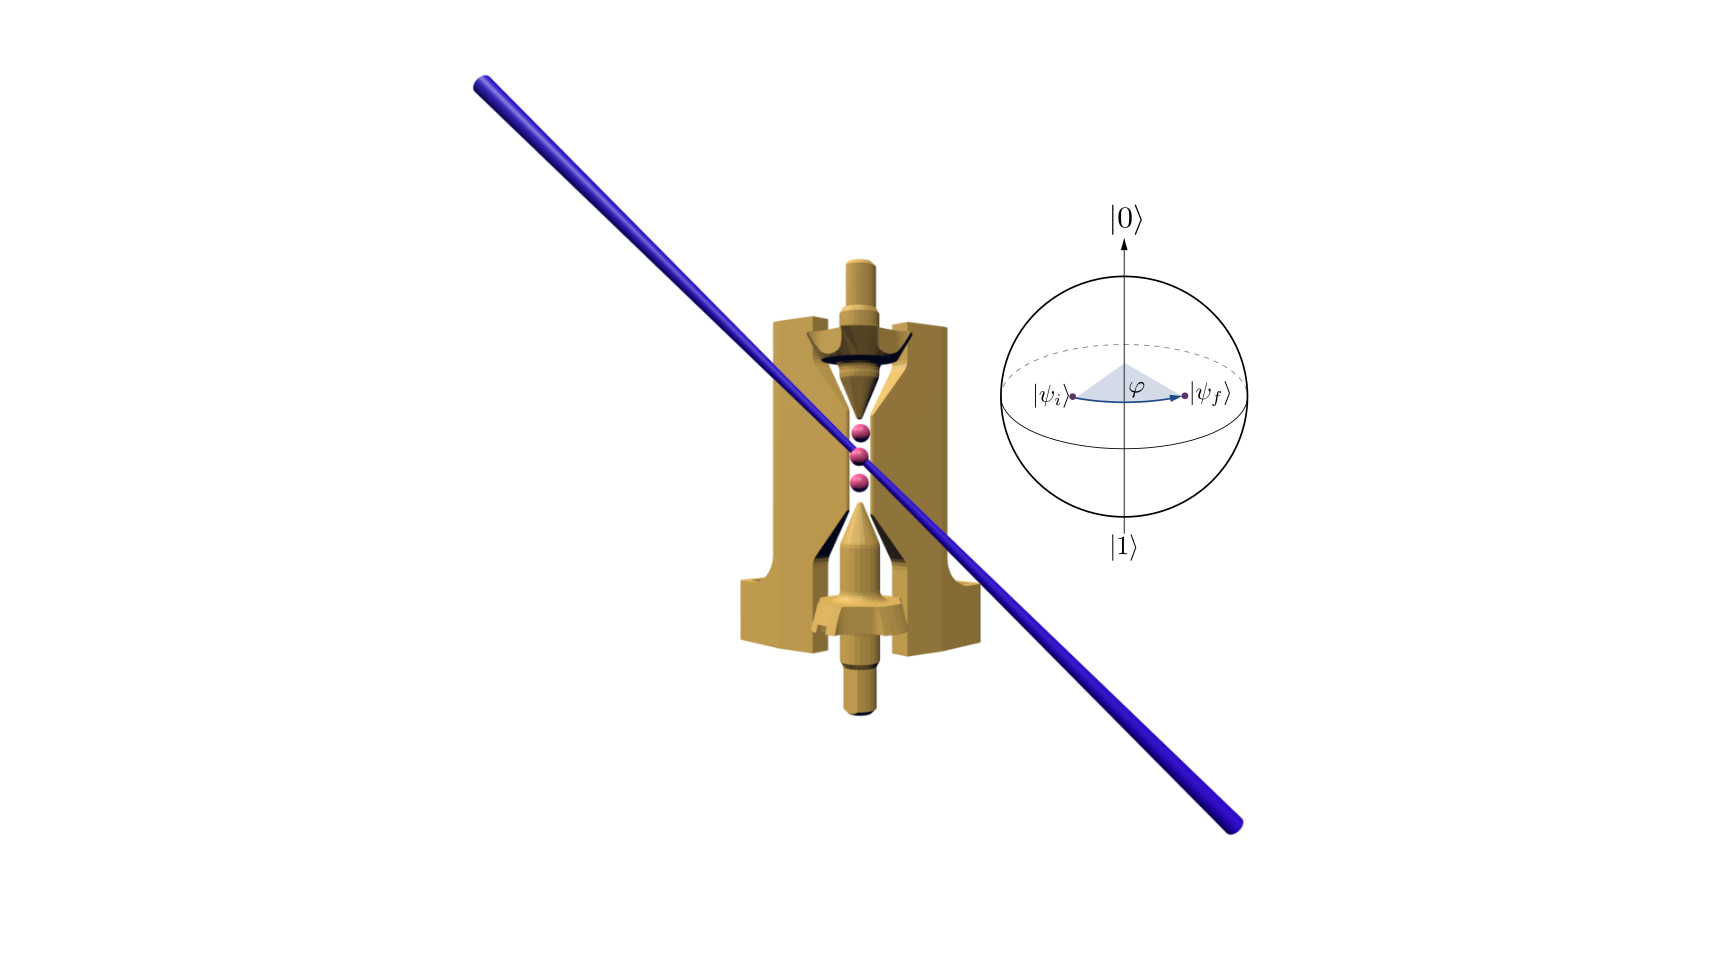
\includegraphics[width=0.4\textwidth]{qubitmanipulation}
  %\caption{Schematic of photon generation}
\end{wrapfigure}
\vspace{-1.4em} The same laser can perform quantum operations on the qubits encoded in the ions. Our goal is to manipulate the state of a single qubit without modifying the state of the others. Here the laser operates in a far-detuned regime, and induces an AC Stark shift on the $\ket{0} = \ket{\text{S}_{j=1/2}, m_j=-1/2}$ state of the ion-qubit implementing a phase gate \cite{chuang}. In order to measure the AC Stark shift we perform a Ramsey interferometry experiment \cite{starkshift}, where between the two $\pi/2$ pulses a detuned Stark pulse is introduced. This pulse shifts the relative phase of the qubit and therefore the amount of Stark shift can be inferred from the final qubit state.

The rest of this thesis is presented in the following way: Chapter 2 is devoted to the theoretical background necessary to understand the rest of the work. Here, the foundations of quantum computing and networking are laid down, along with the basic concepts of ion trapping and Gaussian laser beams; Chapter 3 presents the existing experimental setup, i.e. the already built and working blocks of the experiment where the setup designed in this thesis has been added; Chapter 4 is the core of the thesis, here the final design made with the software Zemax and simulations of different aspects of the project are introduced and presented; Chapter 5 contains all the experimental results obtained. It is divided in two parts: first, the setup was built on an optical table, here we had the freedom to test different key properties of the performance of the system and decide whether or not it was satisfactory. After having the certainty that the system can work as desired, the setup was transferred and aligned on the main experiment where limited access did not allow for easy performance testing. Here, we carried out two experiments that demonstrate the capability of the built system: to manipulate single qubits and generate photons from single ions. The description and discussion of these results are in the second part of chapter 5. Lastly, in Chapter 6 a conclusion with a summary and a future outlook is given.


% Theory chapter
% !TEX root = main.tex

\chapter{Theoretical framework}
Quantum computing is based on a general framework that does not depend on the physical platform. In this chapter, important concepts such as qubits, and quantum operations are described from a theoretical point of view, before showing how we can realize them with trapped ions. The same goes with quantum networking, the concept and the realization can be treated separately and they will be described in this chapter. Furthermore, in this chapter we will take a look into Gaussian beams and their properties. Since that is the shape emitted by laser, it is important to understand their characteristics and how to manipulate them. Lastly, Acousto-optical interactions are introduced and studied to give an idea of how AODs work and how they can be used to steer a laser beam.
\section{Quantum logic with trapped ions}
\subsection{Quantum computer and quantum gates}
\label{sec:quantumoperations}
The concepts of quantum computing are borrowed and extended from classical computational. In the classical case, information is mostly represented in terms of binary digits, the so called bit, essentially mapping information to a base-2 number. Information processing is done with gates acting of those numbers. The idea of a quantum computer is still to encode information in a binary form, but due to the nature of quantum mechanics, a quantum bit (in short qubit) gains new features that can be exploited to perform different kind of operations.\\
A qubit is formally a normalized wave function that can be written as a superposition of two orthogonal states indicated usually with $\ket{0}$ and $\ket{1}$:
\begin{equation}
\label{qubit}
\ket{\psi} = \alpha \ket{0} + \beta\ket{1},
\end{equation}
where $\alpha,\beta$ are probability amplitudes, i.e. two complex numbers that satisfy the relationship $|\alpha|^2+|\beta|^2 = 1$.
A qubit can be in any linear combination, i.e. $\alpha$ and $\beta$. The outcome of measuring a qubit will give the value 0 with a probability of $|\alpha|^2$ and 1 with a probability of $|\beta^2|$.\\
Qubits also have a geometrical representation that can be useful. Equation \eqref{qubit} depends on 4 real numbers, however since $\psi$ is normalized, we can rewrite the expression as
\begin{equation}
\ket{\psi} = e^{i\gamma}\left(\cos\frac{\theta}{2}\ket{0} + e^{i\varphi}\sin\frac{\theta}{2}\ket{1}\right).
\end{equation}
The global phase factor $e^{i\gamma}$ can be left out as it does not influence the measurement outcome, leaving only two real numbers: $\theta$ and $\varphi$. A qubit can therefore be represented geometrically with normalized spherical coordinates. The so called Bloch sphere is depicted in Figure \ref{blochsphere}, every point on its surface represents a different state of the qubit. Here, qubit manipulation can be visualized as trajectories on the surface. The drawback of this representation is that it is limited to only one qubit, so it loses usefulness when dealing with multiple qubits.
\begin{figure}[H]
\centering
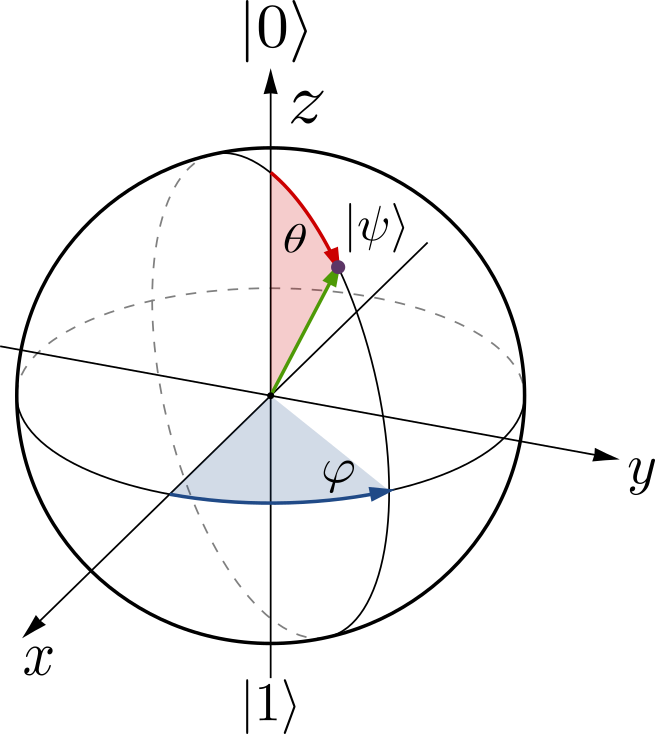
\includegraphics[width = .4\textwidth]{bloch_sphere}
\caption{The Bloch sphere. The states $\ket{0}$ and $\ket{1}$ are at the poles of the sphere, every other point of the surface represents a superpositions of these states. A single qubit quantum gate can be seen as trajectory on the surface mapping one state to another.}
\label{blochsphere}
\end{figure}

An alternative way of dealing with qubits is via vectors and matrices. We can assign to the states $\ket{0}$ and $\ket{1}$ the following:
\begin{equation}
\ket{0} = \begin{pmatrix}
 1 \\
 0
\end{pmatrix} \quad
\ket{1} = \begin{pmatrix}
 0 \\
 1
\end{pmatrix} \implies \ket{\psi} = \begin{pmatrix}
 \alpha \\
 \beta
\end{pmatrix}.
\end{equation}
In this representation, single qubit rotations are calculated using $2\times2$ unitary matrices. These kind of operations are named \emph{quantum gates} and they are the building blocks of quantum computing. Quantum algorithms can be written as a sequence of quantum gates. For a single qubit, any gate can be written as multiple combination of two operations, e.g. \cite{hempel}
\begin{equation}
\label{quantumgates}
U_z(\Theta) =  \begin{pmatrix}
 e^{-i\frac{\Theta}{2}} & 0 \\
 0 & e^{i\frac{\Theta}{2}}
\end{pmatrix} \qquad U_\varphi(\theta) = \begin{pmatrix}
\cos\frac{\theta}{2} & -i e^{-i\varphi}\sin\frac{\theta}{2} \\
-ie^{i\varphi}\sin\frac{\theta}{2} & \cos\frac{\theta}{2}
\end{pmatrix}.
\end{equation}
These two matrices can be seen as two different rotations in the Bloch sphere, $U_z$ is a rotation around the $z$ axis by the angle $\Theta$, while $U_\varphi$ is a rotation around an axis located in the x-y plane. Important examples of single qubit gates are the Hadamard gate $H$, which creates a superposition of one qubit starting from the state $\ket{0}$, or $\ket{1}$, and the phase shift gate $R_\phi$ that shifts the phase:
\begin{equation}
\label{Hadamard}
 H = \frac{1}{\sqrt{2}}\begin{pmatrix}
 1  & 1\\
1 & -1
 \end{pmatrix} \equiv U_{\varphi=\pi}\left(\frac{\pi}{2}\right)U_z(\pi) \qquad R_\phi = \begin{pmatrix}
 1  & 0\\
0 & e^{i\phi}
 \end{pmatrix} \equiv e^{i\varphi/2}U_z(\varphi).
\end{equation}
% As we have seen, a single qubit has already the advantage of superposition compared to classical case. When considering multiple qubits, we gain even more quantum mechanical features like entanglement. This phenomenon does not have a classical analogy and it is an extremely useful tool in quantum information. Let us consider only 2 qubits, a particular case would be
% \begin{equation}
% \ket{\psi} = \frac{1}{\sqrt{2}}\left(\ket{00} + \ket{11}\right).
% \end{equation}
% If a measurement is made on one of the two qubit and, for instance, the outcome is 0, the outcome of a measurement on the second qubit  will be 0 with unit probability. Viceversa, if the outcome of the first measurement was 1, the outcome of the second measurement is always 1.\\
Gates that involve $N$ qubits are written as $2^N\times 2^N$ unitary matrices, a famous example is the controlled not (CNOT) gate
\begin{equation}
\text{CNOT} = \begin{pmatrix}
1  & 0 & 0 & 0\\
0 & 1 & 0 & 0\\
0 & 0& 0 & 1 \\
0 & 0 & 1 &0
\end{pmatrix}.
\end{equation}
It can be shown \cite{chuang} that the examples of this section: $H$ gate, phase gate, and CNOT gate form a universal set of quantum gates, i.e. a sequence of these gates approximates every other quantum gate.

\subsection{Ion qubits and laser-ion interactions}
\label{laserioninteractions}
Qubits can be encoded in any pair of orthogonal quantum states of a physical system. %REWRITE (In the case of an ion it is possible to take two internal electronic states, the qubit is then implemented in their transition. In figure \ref{qubitschemereference} the level scheme of $^{40}\text{Ca}^+$ is presented. The lifetime of the excited level has to be long enough to carry out all the quantum operations without spontaneous scattering. A common choice is the transition $\ket{\text{S}_{1/2}} \to \ket{\text{D}_{5/2}}$, where the ground state $\ket{\text{S}_{1/2}}$ represents the state $\ket{0}$ and the excited state $\ket{\text{D}_{5/2}}$ will be $\ket{1}$).
In Figure \ref{qubitschemereference} the level scheme of $^{40}\text{Ca}^+$ is presented. The states $\ket{\text{S}_{1/2}}$ and $\ket{\text{D}_{5/2}}$ are a common choice to encode a qubit. The ground state $\ket{\text{S}_{1/2}}$ represents the state $\ket{0}$ and the long lived ($\sim$ 1 s) excited state $\ket{\text{D}_{5/2}}$ will be $\ket{1}$. As these levels are directly connected by an electric-quadrupole transition at an optical wavelength (729 nm), this kind of qubit is often referred to as an optical qubit.
Lasers provide a way to directly manipulate the population of these two levels and therefore to manipulate the state of the qubit.\\
The laser set up in this thesis is the 393 nm, which interacts via a dipole transition with the atomic ion, we model therefore the atom-light interactions as dipole interaction. In the case of a quadrupole interaction, the equations below still hold with the exception of the Rabi frequency, which will no longer depend linearly with the electric field. For a proper treatment of the quadrupole interaction see \cite{ross}.\\
%The interaction between ion and laser is now presented using a simple model: a two-level atom with dipole interaction with the laser field.
Consider the system in Figure \ref{2levelatom}, where the states $\ket{0}$ and $\ket{1}$ are separated by a frequency $\omega_0$, while the laser is assumed to be monochromatic with frequency $\omega_l$. The difference $\Delta = \omega_l -\omega_0$ is called detuning and we assume to be in the near resonant regime $\Delta \ll \omega_0$. % The laser light in this case can be described classicaly in the dipole approximation.
%This assumption can be explained as follow, the wavelength of transitions in an atom, are typically in the optical regime: hundreds of nanometers, which is order of magnitude greater then the typical atom dimension. Thus, the electric field can be considered constant over the atom size. This allows to expand the electric field in Taylor series and remove every spatial dependent term in the so called dipole approximation.
The Hamiltonian of the atomic part can be written as:
\begin{equation}
H_a = \hbar\omega_0 \ket{1}\bra{1},
\end{equation}
where $\omega_0$ is the frequency difference between the ground and excited state, the energy of the ground state has also been set to 0. \begin{figure}
\centering
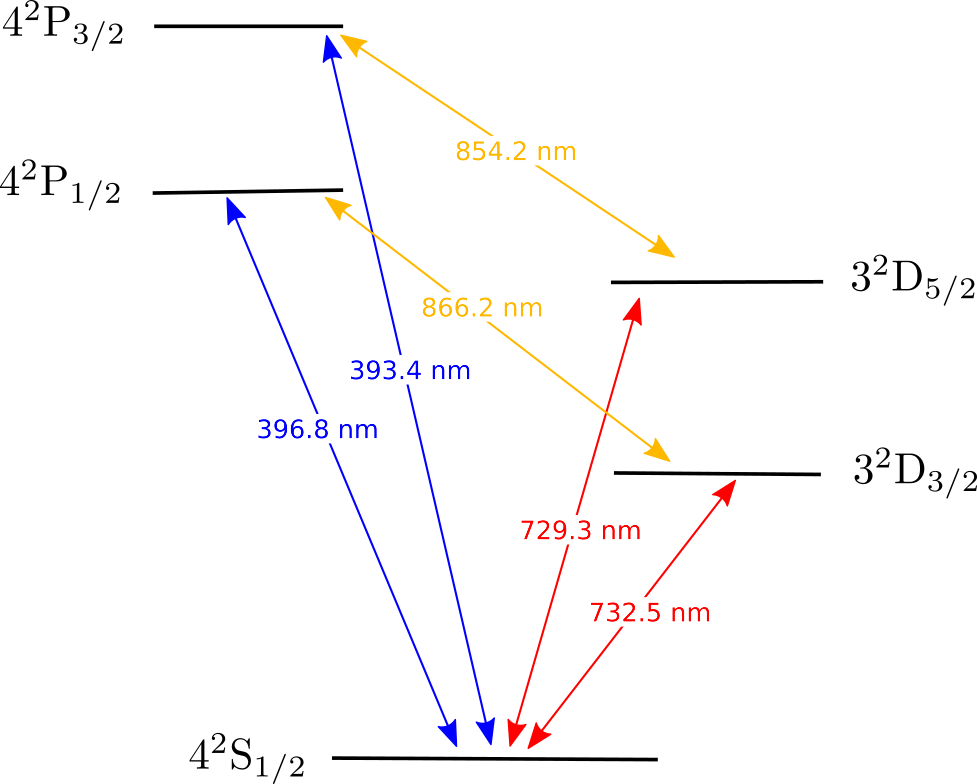
\includegraphics[width = .6 \textwidth]{calciumscheme}
\caption{Level scheme of $^{40}\text{Ca}^+$. Detailed description is in Section \ref{sec:calciumion}. For quantum computing purposes, the chosen qubit transition is the long lived quadropole transition $\ket{\text{S}_{1/2}} \to \ket{\text{D}_{5/2}}$ at 729nm.}
\label{qubitschemereference}
\end{figure}
The Hamiltonian of the interaction between the dipole atomic moment $\mathbf{d}$ and the electric field of the laser can be written \cite{steck}
\begin{equation}
H_{int} = -\mathbf{d}\cdot \mathbf{E}
\end{equation}
where the electric field will be treated classically and the dipole approximation is assumed. This means
\begin{equation}
\mathbf{E}(t) = \hat{\mathbf{\varepsilon}} E_0 \cos(\omega_l t+\varphi) = \hat{\mathbf{\varepsilon}} \frac{E_0}{2} \left(e^{-i(\omega_l t+\varphi)} + e^{i(\omega_l t+\varphi)}\right),
\end{equation}
where $\hat{\varepsilon}$ is the unit polarization vector. The next step is to work out the dipole operator, this can be done by applying the identity $\ket{0}\bra{0} + \ket{1}\bra{1}$ on both sides of $d$. Due to parity arguments \cite{steck}, only the non diagonal terms are non-vanishing, giving
\begin{equation}
d = \braket{0|d|1}\left(\ket{0}\bra{1} + \ket{1}\bra{0}\right) \equiv \braket{0|d|1}(\sigma + \sigma^\dagger).
\end{equation}
Combining the last three equations yields
\begin{equation}
\label{eq:hint}
H_{int} = - \braket{0|\hat{\varepsilon} \mathbf{d}|1}\frac{E_0}{2}(\sigma e^{i(\omega_l t+\varphi)} + \sigma^\dagger e^{-i(\omega_l t+\varphi)} + \sigma e^{-i(\omega_l t+\varphi)} + \sigma^\dagger e^{i(\omega_l t+\varphi)})
\end{equation}
A rotating wave approximation is used now: in the interaction picture, the operator $\sigma$ ($\sigma^\dagger$) evolves under the Hamiltonian $H_a$ in time as $\widetilde{\sigma} = e^{i H_a t/\hbar}\sigma e^{-i H_a t/\hbar} = \sigma e^{-i\omega_0 t}$ ($\widetilde{\sigma}^\dagger=\sigma^\dagger e^{i\omega_0 t}$). Therefore, equation \ref{eq:hint} in the interaction picture contains terms that oscillate as $\propto e^{\pm i(\omega_l-\omega_0 )t}$, and $\propto e^{\pm i(\omega_l+\omega_0 )t}$. We can drop the fast oscillating terms and keeping only those that depend on time as $\propto e^{\pm i(\omega_l-\omega_0 )t}$. The validity of this approximation is given by the fact that $\omega$ and $\omega_0$ are in the optical regime, thus they oscillate extremely fast and average to zero, the interesting slow dynamic is given only by their difference: the detuning.
Going back in the Schrödinger picture yields the final form of the interaction Hamiltonian
\begin{equation}
H_{int} = \frac{\hbar \Omega}{2}(\sigma e^{i(\omega_l t+\varphi)} + \sigma^\dagger e^{-i(\omega_l t+\varphi)}),
\end{equation}
 where we defined the Rabi frequency $\Omega \equiv - \braket{0|\hat{\varepsilon} \mathbf{d}|1}E_0/\hbar$. The Rabi frequency depends linearly with the applied electrical field and hence its square is proportional to the intensity of the laser $\Omega ^2 \propto I$. To summarize, the total system Hamiltonian is
 \begin{equation}
 \label{2levelatomhamiltonian}
H = H_a + H_{int} = \hbar\omega_0 \ket{1}\bra{1} + \frac{\hbar \Omega}{2}(\sigma e^{i(\omega_l t+\varphi)} + \sigma^\dagger e^{-i(\omega_l t+\varphi)}).
 \end{equation}
To eliminate the time dependence, we can go in the rotating frame with the unitary transformation $U = e^{i\omega_l t \ket{1}\bra{1}}$, the Hamiltonian in this frame is
\begin{equation}
\label{Hamiltonianrotatingframe}
\widetilde{H} = -\hbar \Delta \ket{1}\bra{1} + \frac{\hbar \Omega}{2}(e^{i\varphi}\sigma + e^{-i\varphi}\sigma^\dagger)
\end{equation}
\begin{figure}
\centering
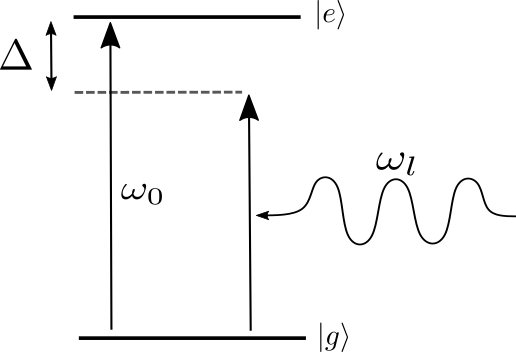
\includegraphics[width = .4\textwidth]{2levelatom}
\caption{2-level atom scheme, the ground and excited states are denoted as $\ket{0}$, and $\ket{1}$. $\omega_l$ is the laser frequency, which is detuned by $\Delta \equiv \omega_l - \omega_0$ from the transition frequency $\omega_0$.}
\label{2levelatom}
\end{figure}
The time dependence is now gone, and the unitary evolution matrix can be calculated as
\begin{equation}
\label{laserpulse}
U(t) = \exp\left\{-\frac{i}{\hbar} \widetilde{H} t \right\} =
 \begin{pmatrix}
  \cos\left(\frac{\widetilde{\Omega} t}{2}\right) + i \frac{\Delta}{\widetilde{\Omega}} \sin\left(\frac{\widetilde{\Omega} t}{2}\right) & -ie^{i\varphi}\frac{\Omega}{\widetilde{\Omega}}  \sin\left(\frac{\widetilde{\Omega} t}{2}\right) \\
  -ie^{-i\varphi}\frac{\Omega}{\widetilde{\Omega}}  \sin\left(\frac{\widetilde{\Omega} t}{2}\right)  & \cos\left(\frac{\widetilde{\Omega} t}{2}\right) - i \frac{\Delta}{\widetilde{\Omega}} \sin\left(\frac{\widetilde{\Omega} t}{2}\right)
\end{pmatrix}.
\end{equation}
Where $\widetilde{\Omega} = \sqrt{\Delta^2 + \Omega^2}$ is the generalized Rabi frequency. In the case of zero detuning ($\Delta = 0$) the matrix is the same as equation \eqref{quantumgates}, thus a resonant laser pulse implements the qubit rotation $U_{\varphi}(\theta)$.\\
As an example, let us take the atom in the ground state $\ket{\psi} = \ket{0}$ and apply the unitary evolution \eqref{laserpulse}. The probability to be in the excited state becomes
\begin{equation}
\mathbb{P}\{\ket{1}\}(t) = |\braket{1|U(t)|0}|^2 = \frac{\Omega^2}{\Omega^2+\Delta^2} \sin^2\left(\frac{\widetilde{\Omega}t}{2} \right)
\end{equation}
This equation is plotted in Figure \ref{rabiflops}. For $\Delta = 0$, we get a cosine behaviour, the so called Rabi oscillations. The probability amplitude for the electron, under continuous drive by a laser, will oscillate between the ground and excited state at a frequency $\Omega/2$. Detuning damps the amplitude of such oscillations and increases the oscillation frequency. Rabi oscillations are an important tool in quantum information, laser pulses can prepare the state of the qubit in any superposition, e.g. starting in the $\ket{0}$ state, a $\pi/2$ pulse ($\Omega t = \pi/2$ and phase $\varphi=0$) will result in the state $(\ket{0} - i\ket{1})/\sqrt{2}$, with a $\pi$ pulse ($\Omega t = \pi$, $\varphi=\pi$) the population is completely transferred to another level $\ket{0}\to \ket{1}$. These pulses can be used to implement e.g. the Hadamard gate of equation \eqref{Hadamard}.
\begin{figure}[H]
\centering
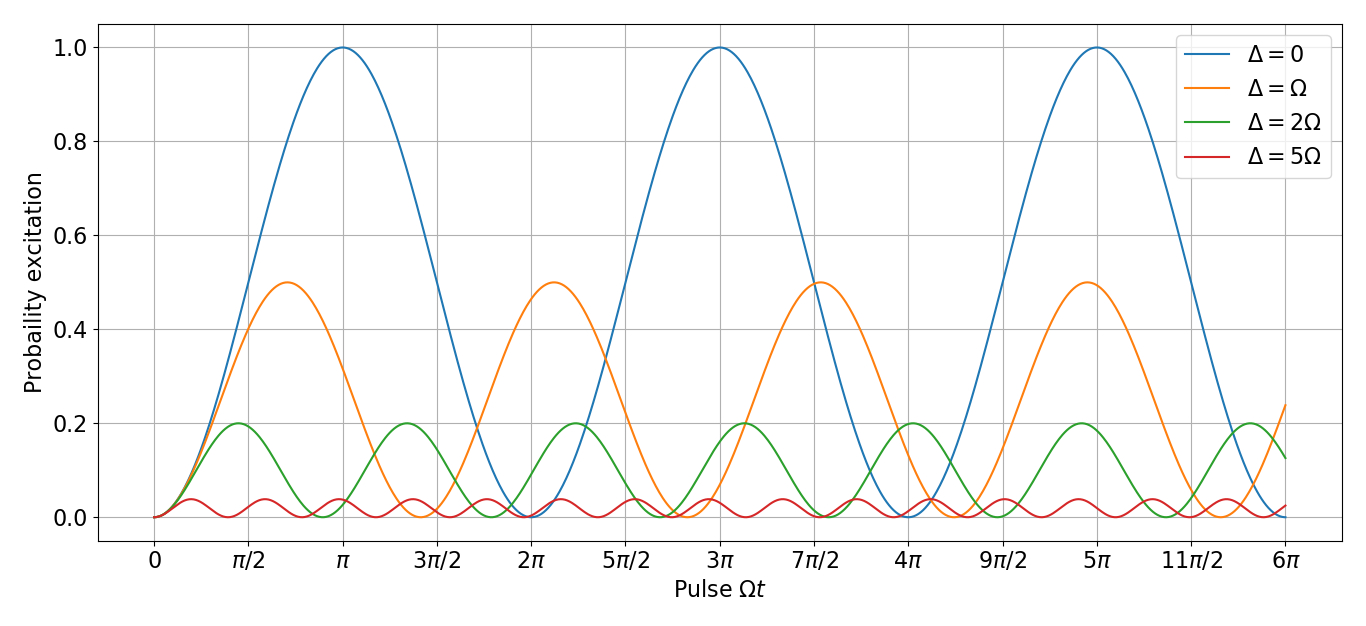
\includegraphics[width = 1\textwidth]{rabiflops}
\caption{Rabi flops for different detunings $\Delta$, starting from the $\ket{0}$ state.}
\label{rabiflops}
\end{figure}
As the light is detuned from the transition, Rabi oscillations are suppressed: the amplitude is reduced by a factor of 0.5 already with $\Delta = \Omega$, while a factor of 10 in reduction is achieved with a detuning of $\Delta = 5\Omega$. However, another effect occurs in the off-resonant regime, the energy levels are shifted.
The shift $\delta$ can be calculated by finding the eigenvalues of the Hamiltonian \eqref{Hamiltonianrotatingframe}, which can be written in matrix form and diagonalized. We find that there are two eigenstates $\ket{+}$ and $\ket{-}$ called dressed states with eigenvalues
\begin{equation}
E_{\pm} = -\frac{\hbar\Delta}{2} \pm \frac{\hbar}{2}\sqrt{\Delta^2 +\Omega^2}.
\end{equation}
In the limit $\Delta \gg \Omega$, dressed states tend to the bare states $\ket{+} \to \ket{1},\ket{-}\to \ket{0}$, and the energies become
\begin{equation}
\label{eq:starkshift}
E_{\pm} \to -\frac{\hbar \Omega}{2} \pm \frac{\hbar \Omega}{2} \pm \frac{\hbar \Omega^2}{4\Delta} \implies \delta = \pm\frac{\Omega^2}{4\Delta}.
\end{equation}
The effective Hamiltonian for the off-resonant regime can be derived following a Markovian approximation \cite{acstarkhamiltonian}
\begin{equation}
H_{AC} = \frac{1}{\hbar \Delta} [\sigma,\sigma^\dagger] = \frac{\hbar \delta}{2}\sigma_z
\end{equation}
The corresponding evolution is
\begin{equation}
\label{acstarkrotation}
U(t) = \exp\left\{-\frac{i}{\hbar} H_{AC} t \right\} =
 \begin{pmatrix}
   \exp\left\{i\frac{\delta}{2}t\right\} & 0\\
   0 & \exp\left\{i\frac{\delta}{2}t\right\}
\end{pmatrix}.
\end{equation}
This matrix implements the quantum gate $U_z(\Theta)$ from equation \eqref{quantumgates}.


\subsubsection{Three-level model}
\label{sec:threelevel}
\begin{figure}
\centering
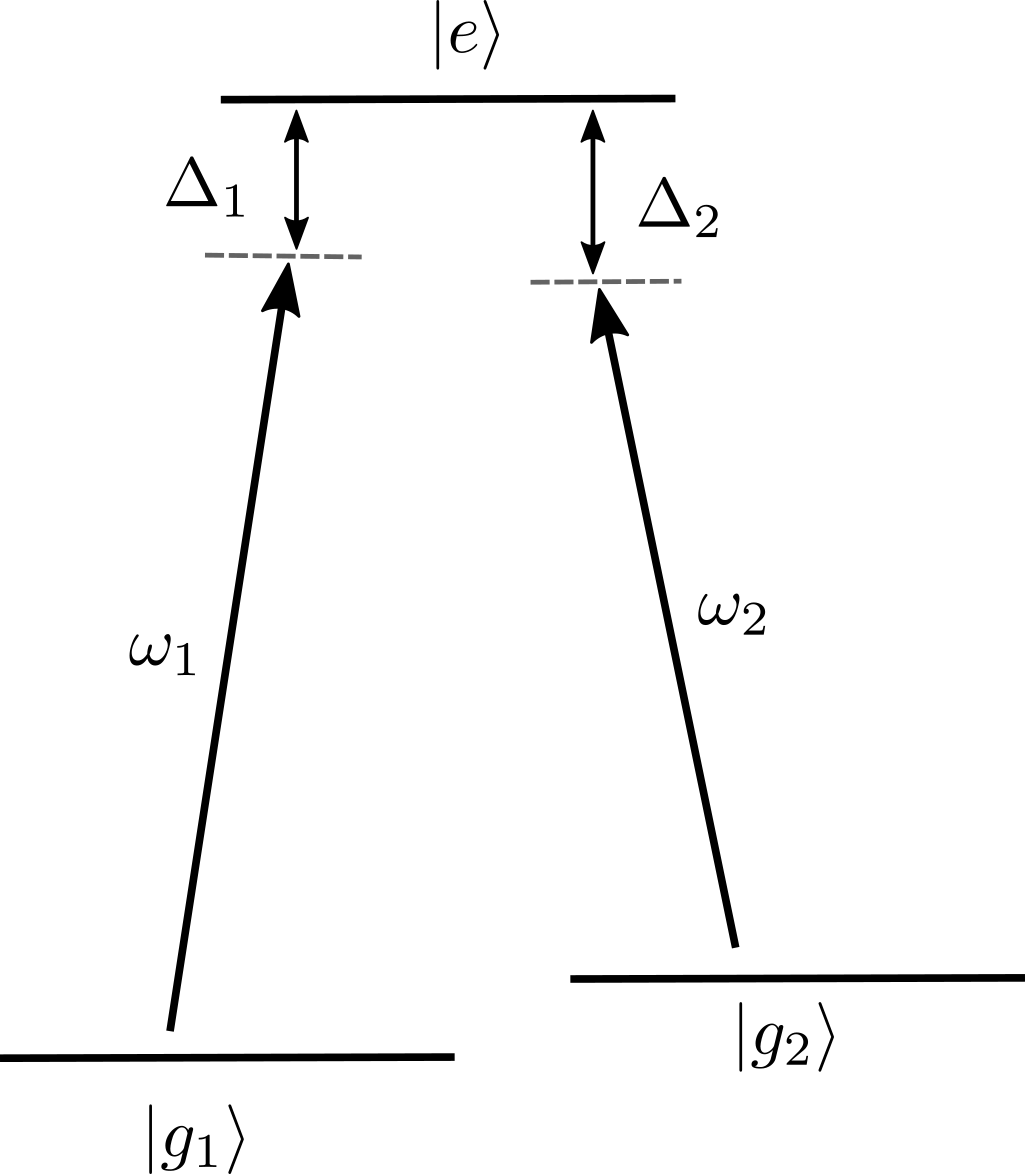
\includegraphics[width = .3\textwidth]{3levelmodel}
\caption{3 level atom model. Two long lived ground states $\ket{g_1}$, $\ket{g_2}$ couple to an excited level $\ket{e}$ through two lasers of frequencies $\omega_1$, $\omega_2$ detuned respectively $\Delta_1,\Delta_2$ from the transitions.}
\label{3levelmodel}
\end{figure}
We extend our model to a 3 level $\Lambda$ type atom driven by two lasers, which closer resemble the real experimental situation in the experiments in this thesis. The model contains new effects that explain photon generation and qubit gates. In particular, stimulated Raman transition will be discussed, and we will show how, under certain conditions, the system can be approximated as an effective 2 level atom. The system is depicted in Figure \ref{3levelmodel}, two ground states $\ket{g_1}$ and $\ket{g_2}$ are present together with a common excited state $\ket{e}$. Two different lasers $\omega_1,\omega_2$ drive the transition $\ket{g_1} \to \ket{e}$ and $\ket{g_2} \to \ket{e}$, where the atomic frequencies are $\omega_{01}$, and $\omega_{02}$ respectively. Detunings are defined as $\Delta_1 = \omega_1 - \omega_{01}$ and $\Delta_2 = \omega_2 - \omega_{02}$. In the case of calcium, the ground states are $\ket{\text{S}_{1/2}}$, and $\ket{\text{D}_{5/2}}$. This is the qubit transition, and it is long lived ($\sim 1$ s), such that any spontaneous emission from D to S can be neglected. The excited level is $\ket{\text{P}_{3/2}}$ which can decay into both ground states with branch ratio of 94\% from P$\to$S ($\sim$ 7.4 ns) and 5.3\% from P$\to$D $\sim 101$ ns), we neglet decay to the $\ket{\text{D}_{3/2}}$ state.\\
%In this model we assume that each laser light couples only to one transition and that . %the two ground states are not separated by an optical frequency $\omega_{02} - \omega_{01} \ll \omega_1,\omega_2$, and that the detunings are nearly equal $\Delta_1 \simeq \Delta_2$. As a consequence, each laser light couples only to one transition.\\
Following the approach of \cite{steck}, the bare atom Hamiltonian is
\begin{equation}
H_a = -\hbar \omega_{01}\ket{g_1}\bra{g_1} - \hbar \omega_{02}\ket{g_2}\bra{g_2},
\end{equation}
with the convention of setting the excited level energy to 0. The electric field is now the sum of the two laser fields
\begin{equation}
\mathbf{E}(t) = \hat{\varepsilon_{01}} E_{01} \cos(\omega_{1} t \varphi_1) + \hat{\varepsilon_{02}} E_{02} \cos(\omega_2 t + \varphi_2).
\end{equation}
As in Section \ref{laserioninteractions}, we then consider a dipole interaction, make the dipole approximation and a rotating wave approximation. Finally, the full final Hamiltonian in the rotating frame is
\begin{equation}
H = \hbar \Delta_1 \ket{g_1}\bra{g_1} + \hbar\Delta_2 \ket{g_2}\bra{g_2}+ \frac{\hbar \Omega_1}{2}\left(\sigma_1 e^{i\varphi_1} +\sigma_1^\dagger e^{i\varphi_1}\right)+ \frac{\hbar \Omega_2}{2}\left(\sigma_2 e^{i\varphi_2} +\sigma_2^\dagger e^{i\varphi_2}\right),
\end{equation}
where $\Omega_i = -\frac{\braket{g_1|\varepsilon_i \cdot \mathbf{d}|e}E_{i}}{\hbar}$, and $\sigma_i = \ket{g_i}\bra{e}$. Under certain conditions, this Hamiltonian describes a Raman process, where state population is transferred coherently between $\ket{g_1}$ and $\ket{g_2}$. Specifically, the Raman conditions are: equal detunings $\Delta_1 = \Delta_2 \equiv \Delta$ (Raman resonance), and $\Delta \gg \Omega_1,\Omega_2$.
Intuitively, this corresponds to the situation where the difference of the two driving frequencies $(\omega_1-\omega_2)$ is equal to the frequency splitting between $\ket{g_1}$, and $\ket{g_2}$.\\
Following \cite{russo} it can be shown that, under the previous conditions, the Raman process leads to an effective coupling directly between the two ground states. The effective Rabi frequency of the coherent population transfer $\ket{g_1} \to \ket{g_2}$ is \cite{steck}
\begin{equation}
\label{eq:effectiverabi}
\Omega_{eff} = \frac{\Omega_1\Omega_2}{2\Delta}.
\end{equation}

\subsubsection{Dissipative processes}
\label{sec:dissipation}
In our experiments spontaneous emission can play a role as the condition $\Delta \gg \Omega_1,\Omega_2$ is only partially fulfilled. In this section therefore, we present a quantitative overview of spontaneous scattering as a function of detuning and Rabi frequency of each laser. In general, dissipative processes do not follow a Hermitian evolution, hence their mathematical description is done heuristically by adding terms in the Heisenberg equation
\begin{equation}
\label{masterequation}
\frac{d\rho}{dt} = \frac{1}{i\hbar}[H,\rho] + \mathcal{L}(\rho).
\end{equation}
This equation is usually referred to as master equation in Lindblad form, where $\rho$ is the density matrix of the system. The superoperator
$\mathcal{L}(\rho)$ contains phenomena not included in the Hamiltonian. For spontaneous emission, the form of $\mathcal{L}(\rho)$ is \cite{quantumnoise}
\begin{equation}
\mathcal{L}(\rho) = \frac{\Gamma}{2}(2\sigma \rho \sigma^\dagger -\sigma^\dagger\sigma \rho - \rho \sigma^\dagger \sigma),
\end{equation}
where $\Gamma$ is the spontaneous emission rate.
% The master equation \eqref{masterequation} can be explicitly written for every component of the density matrix $\rho$,
%in the rotating frame they are called optical Bloch equations. The solution for the excited population in the case of the 2 level atom shows that the effect of spontaneous emission is to damp Rabi oscillations.
For the three level atom, in the effective 2 level system picture, the spontaneous emission is modified as \cite{russo}
\begin{equation}
\label{eq:gammaeff}
\Gamma_{eff} = \left(\frac{\Omega_1}{2 \Delta_1}\right)^2 \cdot \Gamma.
\end{equation}
The ratio between $\Gamma_{eff}$ and the AC Stark shift \eqref{eq:starkshift} $\delta/\Gamma_{eff}\propto \Delta$ dictates which effect is dominant, i.e. by increasing the detuning, the effective rate of spontaneous scattering can be reduced in favor of the AC Stark shift. This regime can be used to implement a phase gate where the qubit is encoded in the $\ket{g_1}\to\ket{g_2}$ transition and the phase of $\ket{g_1}$ is manipulated by Stark shifting the transition $\ket{g_1}\to \ket{e}$. In the experiment of Section \ref{sec:singlequbitmanipulation}, we implement this gate on a single ion in a string.


\section{Quantum networking with trapped ions}
\subsection{General introduction}
A quantum network is a collection of quantum processors, referred to as nodes, interconnected with quantum channels, referred to as links. Nodes are used for processing and storing quantum information, while links for quantum information distribution \cite{kimble}. %Quantum channels are able to transmit quantum states between the nodes and thereby distribute entanglement between the nodes of the network \cite{kimble}.
% There are two classes of quantum networks which are differentiated by the purpose, networks can be used for transmission of information, i.e. communication, or for distributed quantum computation, i.e. scaling of quantum processors \cite{ion_quantumnetwork}.
%In these two cases the topology of the network is different, but the core elements are the same: a node, where quantum information is prepared, manipulated, and stored; and a link that connects nodes.
Applications of quantum networks are several: secure communication with Quantum Key Distribution, clock synchronization, efficient solutions to distributed system problems, and more \cite{Wehnereaam9288}.\\
Links are typically realized with traveling photons, either in free-space \cite{Hughes2002} or in optical fibers. Nodes can be realized using different physical systems: trapped ions \cite{ion_quantumnetwork}, neutral atoms \cite{Ritter2012}, atomic ensembles \cite{kimble}. Nodes and links are connected through an interface that converts a stationary qubit in a node to a flying qubit over the network.  In the next section we will explore how such an interface can be realized by placing an ion-qubit in an optical cavity.\\
Faithful transmission of quantum states over long distances can be a daunting problem as quantum information cannot be cloned \cite{nocloning} and noisy channels can destroy the delicate nature of qubits. Quantum repeaters have been designed \cite{quantumrepeters} to circumvent these problems through a series of protocols which include entanglement purification, a form of error correction \cite{Pan2001}. Once entanglement has been established between nodes, other network functionalities become available, like for instance teleportation \cite{PhysRevLett.70.1895}. Entanglement generation, and quantum repeaters are just some examples of the fundamental steps necessary for building a quantum network, for a more in depth review look at \cite{Wehnereaam9288}.


\subsection{Cavity QED}
\label{sec:cavityqed}
A single trapped ion is a single photon source and those photons can be collected either with a lens \cite{ion_quantumnetwork}, refocused with mirrors \cite{PhysRevLett.120.193603} or with optical cavities \cite{Keller2004bis}. Photon collection from ions using an optical cavity is a powerful approach, that will now be introduced in detail. A cavity placed around ions improves the efficiency of photon collection as the probability of a photon to be emitted in the cavity mode is enhanced with respect to emitting in free space \cite{Kimble_1998}.\\
In this Section a simple model of a two-level system in a cavity is described following the approach of \cite{steck}. We described the cavity electric field as quantized, with $a,a^\dagger$ the creation and annihilation operators of a single photon in the cavity mode, respectively.
The quantized electric field assumes the form of
\begin{equation}
\mathbf{E} = A(\mathbf{f}(\mathbf{r})a + \mathbf{f}^*(\mathbf{r})a^\dagger)
\end{equation}
where $A$ is an amplitude, and $\mathbf{f}(\mathbf{r})$ is the spatial mode profile. The interaction between the dipole moment of a two-level atom and the cavity field is in the dipole form
\begin{equation}
H_{int}  = -\mathbf{d}\cdot \mathbf{E} = \hbar g (\sigma a^\dagger + \sigma^\dagger a),
\end{equation}
where $g = A \braket{0|\mathbf{d}|1}\cdot \mathbf{f}(\mathbf{r})$ is called the cavity coupling constant, it is analogous to the Rabi frequency. An important dependence of $g$ can be found by considering that $f(r)$ is inversely proportional to the volume of the cavity $V$, i.e.
\begin{equation}
g \propto \braket{0|d|1} \sqrt{\frac{\omega}{2\varepsilon_0 \hbar V}}.
\end{equation}
The coupling therefore increases with decreasing cavity volume.\\
The total system Hamiltonian includes also the atomic part, and the free evolution of the cavity single mode field, it takes the name of Jaynes-Cummings Hamiltonian and it is written as \cite{qedreview}
\begin{equation}
\label{eq:jchamiltonian}
H = \hbar \omega_0 \ket{1}\bra{1} + \hbar \omega a^\dagger a + \hbar g (\sigma a^\dagger + \sigma^\dagger a).
\end{equation}
We are interested in comparing the coherent process in \eqref{eq:jchamiltonian} with: spontaneous emission in a free space field mode, and decay in one cavity mode and out of the cavity. The first is quantified with the decay rate $\Gamma = 2\gamma$, while the latter is characterized by the decay rate $\kappa$ (half width half maximum). The decay rate $\kappa$ depends exclusively on the cavity parameters as \cite{helene}
\begin{equation}
\kappa =\frac{c\pi}{FL},
\end{equation}
where $F$ is the cavity finesse, and $L$ the length. % The cavity length is actively stabilized with a PDH type feedback which locks the mirrors position to a 806nm laser. One mirror of the cavity is highly reflective $T_1 = 2.2$ ppm, while the other is more transmissive $T_2 = 97$. This asymmetry of the mirrors allows for the produced photons to exit one from one side in most cases and subsequently coupled to a fiber. The probability to get a photon out of the cavity from the designed mirror can be determined from the transmission and losses of the cavity, the maximum achievable is $P_{max} = 0.83$. The maximum $g$ factor achievable with this geometry is $g = 2\pi \times 1.53$ MHz.
\subsection{Photon generation}
\label{sec:ramanprocess}
In our experiments, photons are generated from an ion-cavity system. Photons generation involves three levels and occurs via the Raman process described in Section \ref{sec:threelevel}. However, here the second laser is replaced by the vacuum electric field of the cavity in a process known as cavity-mediated Raman Process (CMRP) \cite{stuteinterface}. In Figure \ref{ramanprocess} the relevant calcium levels for the CMRP are displayed. A possible choice for the three levels is
\begin{equation}
\ket{\text{S}_{1/2},-1/2}\to\ket{\text{P}_{3/2},-3/2} \to \ket{\text{D}_{5/2},-5/2}.
\end{equation}
In this case the transitions strengths, i.e. the projection of the laser polarization onto the dipole moment, and the same projection onto the cavity axis are maximized over all other choices of transitions for the CMRP \cite{stuteinterface}. A single laser pulse with strength $\Omega$ couples the $\text{S}_{1/2}$ level to the $\text{P}_{3/2}$ level, which is coupled to the $\text{D}_{5/2}$ via the vacuum mode of the cavity. Therefore, the electron state is transferred from the state $\ket{\text{S}_{1/2}} \to \ket{\text{D}_{5/2}}$  by absorbing a laser photon and emitting a photon into the cavity. The final state is therefore $\ket{\text{D}_{5/2}}\ket{1}$, where $\ket{1}$ indicates one photon in the cavity. Afterwards, the photon leaves the cavity leaving the system in the $\ket{\text{D}_{5/2}}\ket{0}$ state. The effective Rabi frequency \eqref{eq:effectiverabi} of the population transfer is modified as \cite{Barros2009}
\begin{equation}
\label{omegaeff}
\Omega_{eff} = \frac{\Omega g}{\Delta},
\end{equation}
where the Rabi frequency of the second laser is now replaced by the atom cavity coupling $g$. The Raman resonance appears when the detuning $\Delta$ of the laser and the cavity are the same. The effective spontaneous decay rate from this level is from equation \eqref{eq:gammaeff}
\begin{equation}
\Gamma_{eff} = \left(\frac{\Omega}{2\Delta}\right)^2\Gamma
\end{equation}
The effective Rabi frequency $\Omega_{eff}$ and the effective spontaneous decay $\Gamma_{eff}$ are competitive effects and the ratio of the two depends on the detuning $\Omega_{eff}/\Gamma_{eff} \propto \Delta/\Omega$. It is therefore possible to reduce spontaneous emission effects if the detuning is large enough.\\
In our experiment the designed cavity is near concentric with a length of $L = 19.9$ mm. The maximum $g$ factor achievable with this geometry is $g_{max} = 2\pi \times 1.53$ MHz, while the decay rate is $\kappa = 2\pi\times 70$ kHz. More information on our cavity can be found in \cite{Krutyanskiy2019} and in the upcoming thesis of J. Schupp. Typical numbers in our experiment for the CMRP are $\Omega =  2\pi\times 40$ MHz, detuning $\Delta = 2\pi\times 400$ MHz, $g = 2\pi\times 1$ MHz, and from table \ref{transitiontable}, $\Gamma = 2\pi \times 21.4$ MHz. With these conditions we have
\[\Omega_{eff} \sim 2\pi\times 100\, \text{kHz} > \Gamma_{eff} \sim 2\pi\times 53\,\text{kHz}.\]
The regime we work in is thus $2\kappa>\Omega_{eff}>\Gamma_{eff}$. In Section \ref{exp:photons}, we use the single-ion focused Raman laser, developed in this thesis, to implement the CMRP on a single ion in a string.
\begin{figure}
     \centering
     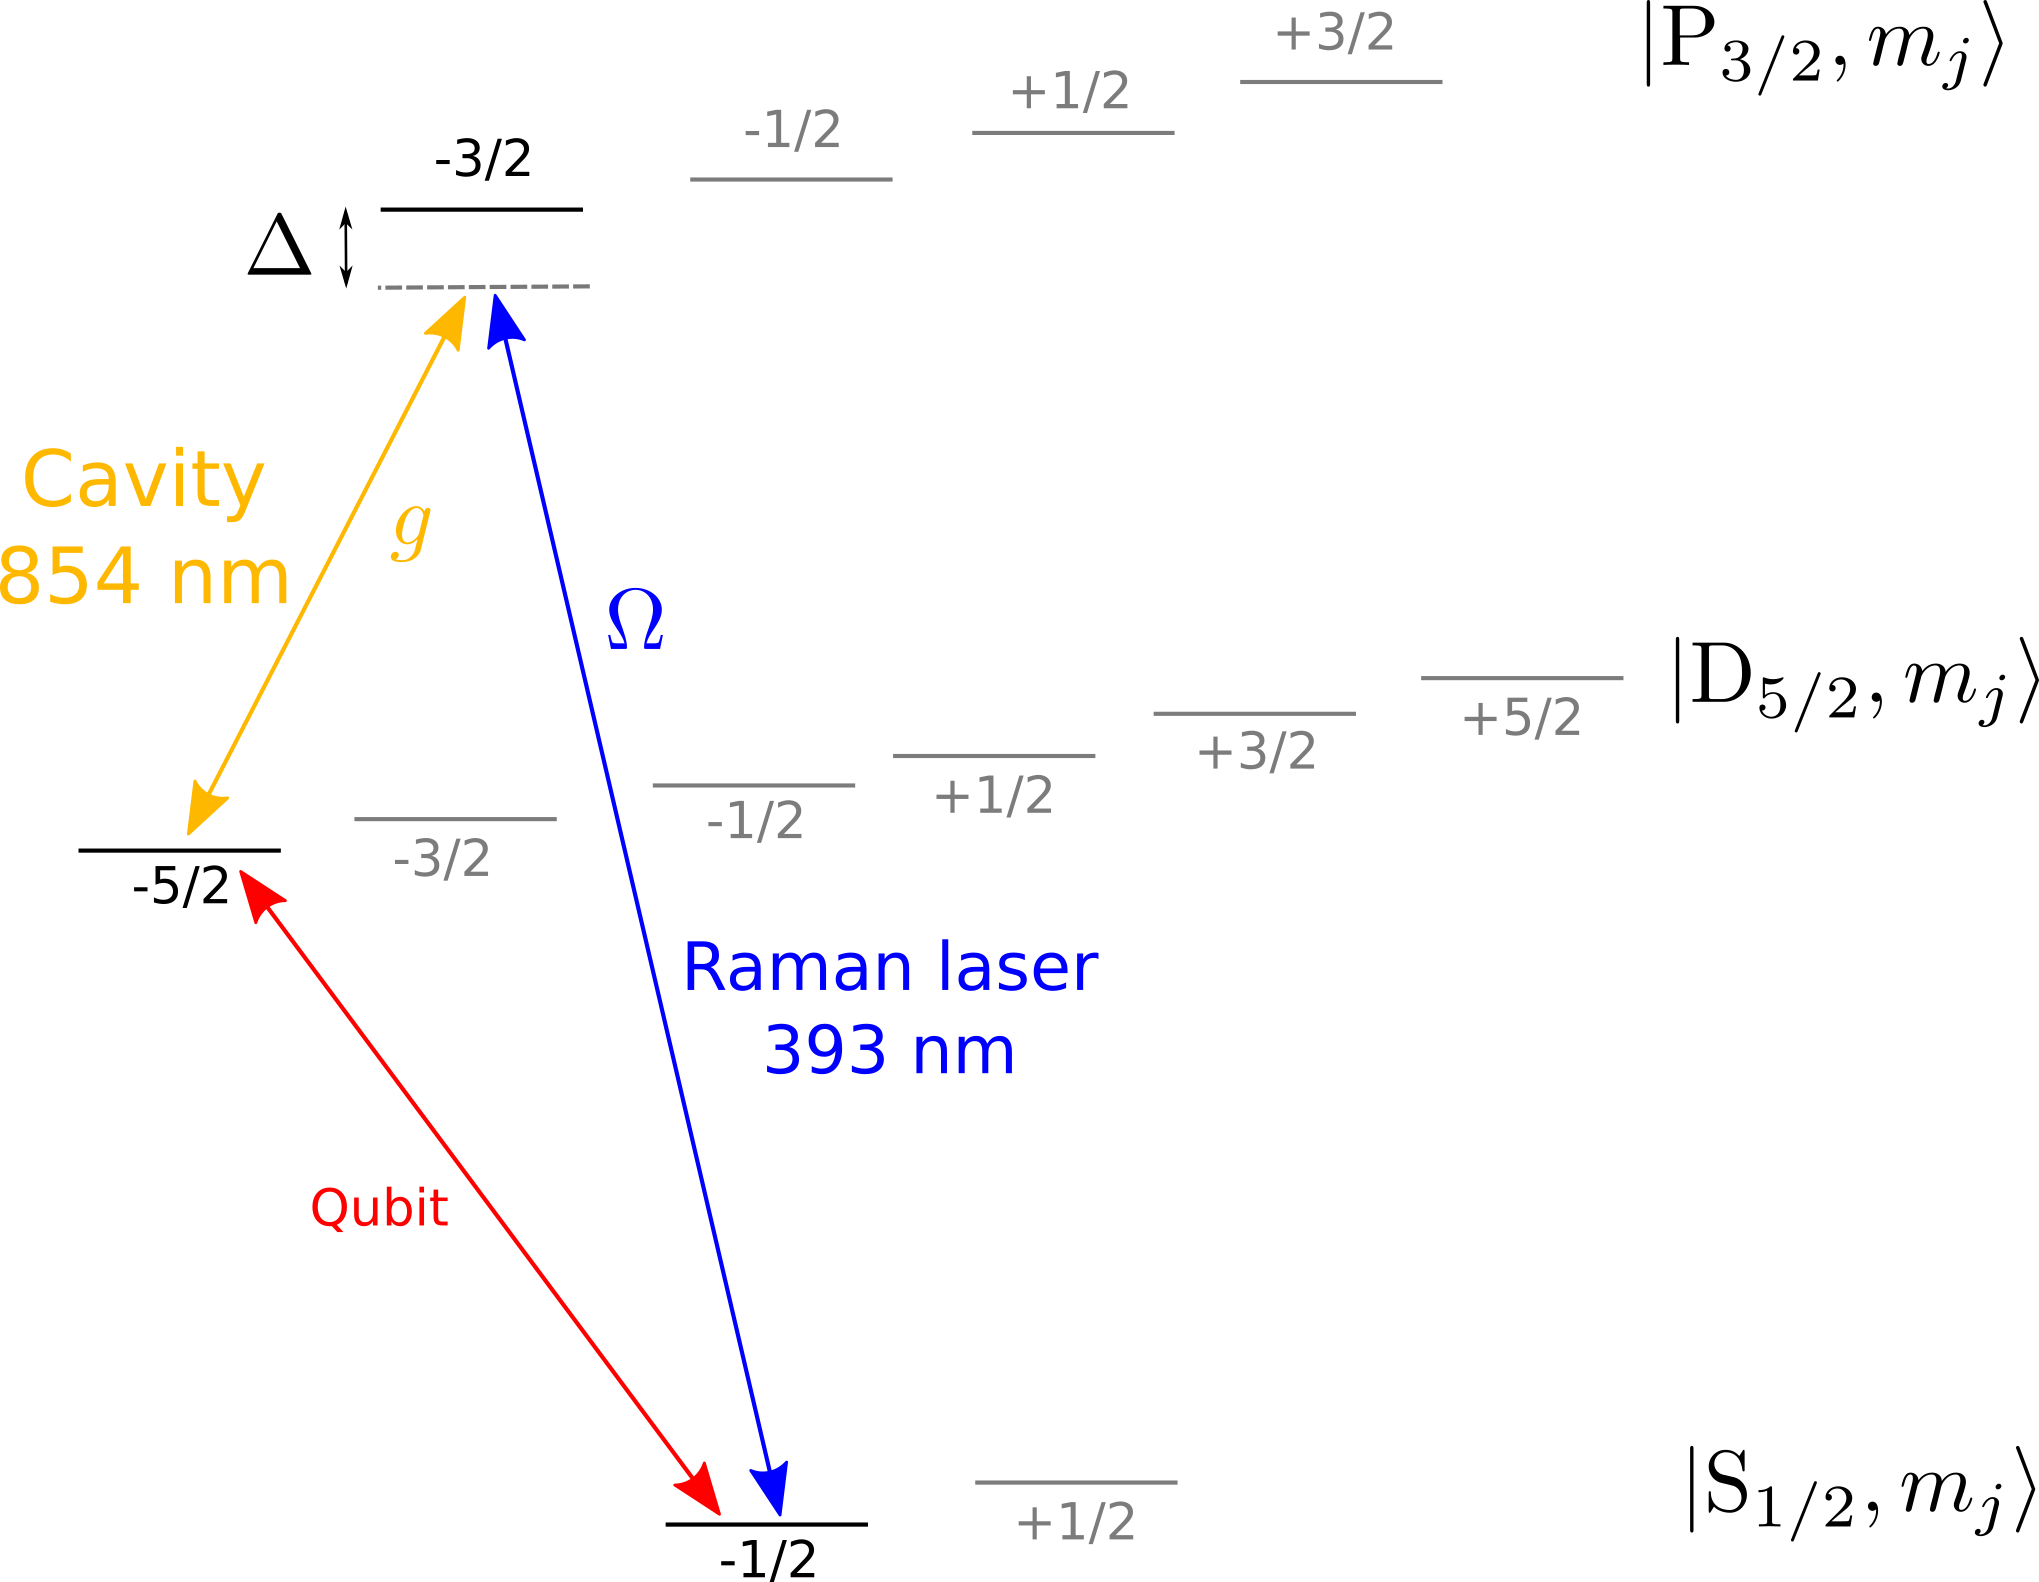
\includegraphics[width=.6\textwidth]{photongenerationscheme}
    \caption{Displayed is the Zeeman structure of the relevant manifolds of calcium for the cavity-mediated Raman process. Here only one choice for the Zeeman level is depicted, but other are also possible. If the cavity and the Raman laser have the same detuning $\Delta$, an electron in the ground state $\ket{\text{S}_{1/2}}$ absorbs a 393 nm photon and ends in the $\ket{\text{D}_{5/2}}$ state after emitting a 854 nm photon in the cavity.}
      \label{ramanprocess}
\end{figure}

% The generated photon can then be used for quantum networking purposes, this requires also the possibility to entangle the ion with the generated photon, which can be done by driving the CMRT with a bichromatic beam \cite{ionphotonentanglement}.

%In the real experiment the designed cavity is near concentric with a length of $19.9$ mm, and radii of curvature of $9.98$ mm. The cavity length is actively stabilized with a PDH type feedback which locks the mirrors position to a 806nm laser. One mirror of the cavity is highly reflective $T_1 = 2.2$ ppm, while the other is more transmissive $T_2 = 97$. This asymmetry of the mirrors allows for the produced photons to exit one from one side in most cases and subsequently coupled to a fiber. The probability to get a photon out of the cavity from the designed mirror can be determined from the transmission and losses of the cavity, the maximum achievable is $P_{max} = 0.83$. The maximum $g$ factor achievable with this geometry is $g = 2\pi \times 1.53$ MHz.

% The Finesse of the cavity for the TEM$_{00}$ mode is 54000. The other cavity parameters are $\kappa = 2\pi \times 70$ kHz, and $\gamma = 2\pi\times 11.45$ MHz for the $\text{P}_{3/2}$ state. With these numbers the preferred strong regime is not reached, but nonetheless,  it is still possible to produce photons and collect them out of the cavity.

\section{Basics of ion trapping}
\subsection{Linear Paul trap}
Ions are charged, therefore electric fields can be used to control and trap them. In order to achieve confinement in 3 dimensions, a potential $\phi(x,y,z)$ with minima in all directions is needed. However, it follows directly from Maxwell's equations $\nabla^2 \phi = 0$ that the potential must be antitrapping at least in one direction. There are two workarounds for this problem: the first one introduces magnetic fields to trap particles in some directions, this takes the name of Penning trap \cite{RevModPhys.58.233}. The second solution is the so called Paul trap, and it is what we are going to describe in this section. The idea is to introduce a time varying potential, such that the antitrapping direction is constantly switching between two different dimensions. The particles will therefore experience an effective confinement in all directions if the switching is fast compared to the time it takes the particle to respond.\\
The shape of the trap can be adapted to load more ions in different geometries. In our work we utilize a linear Paul trap, which is elongated in one direction. The confinement in this direction is weaker and thus loaded ions will align in a single long string. This kind of trap is depicted in Figure \ref{trap}.
\begin{figure}
\centering
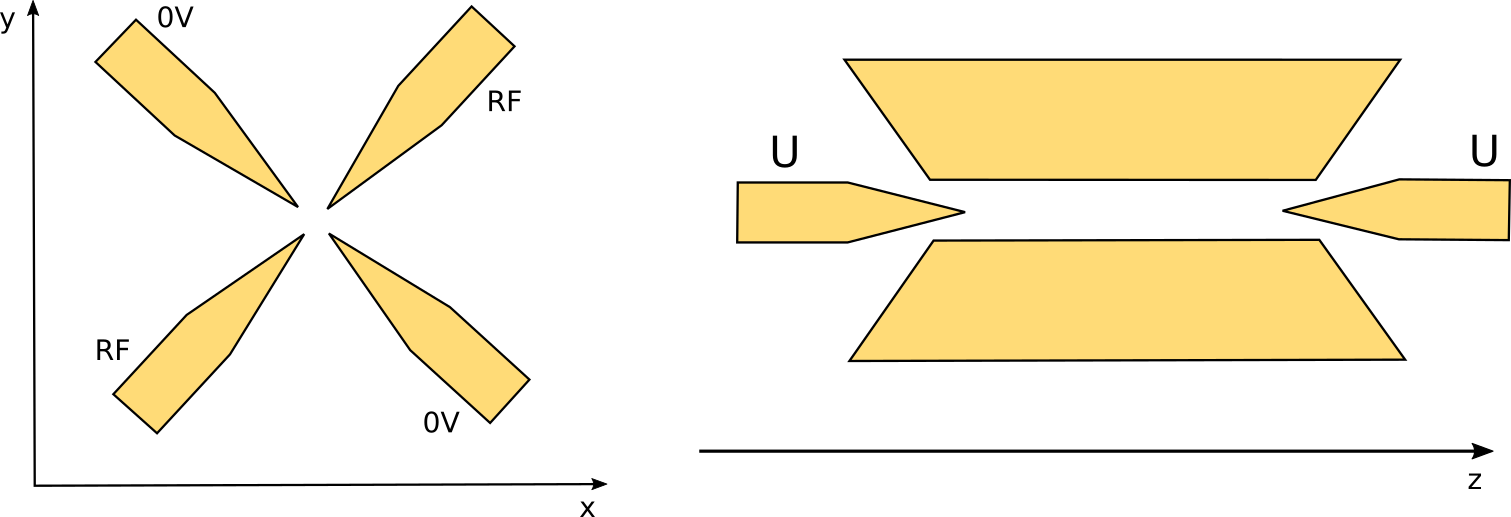
\includegraphics[width = .7\textwidth]{trap}
\caption{A linear paul trap. U is the voltage applied to the electrodes trapping in the $z$ direction, while in the $x-y$ plane trapping is achieved with a radio frequency signal.}
\label{trap}
\end{figure}
The confinement in the $x-y$ plane is provided by 4 electrodes, two of which are grounded and the other two are connected to a radio frequency source. This design is similar to a mass filter, with the difference of additional endcaps electrodes in the $z$ direction that plug the trap and confine also in the axial direction.\\
The potential inside the trap can be described for the $x-y$ plan independently from the $z$ direction. In the case of a linear Paul trap the radial potential is \cite{traptheory}:
\begin{equation}
\phi  = \frac{\Phi_0}{2r_0^2}\left(x^2 - y^2\right),
\end{equation}
where $r_0$ is the distance from the center of the trap to the electrodes. The amplitude consists of a static part $U_0$ and a dynamical one $\Phi_0 = U_0 + V \cos(\Omega_{RF} t)$.
The study of the particle's motion with mass $m$ and charge $e$ inside the trap can be done with classical physics, Newton's second law in this case is
\begin{equation}
m\ddot{x} = -q \frac{\partial \phi}{\partial x} = - \frac{ex}{r_0^2}\left(U_0 + V \cos(\Omega_{RF} t) \right),
\end{equation}
and similarly for $\ddot{y}$. This equation can be written in the form of Mathieu equation \cite{Richards1983} by defining two parameters:
\begin{equation}
a_x = \frac{4eU_0}{\Omega_{RF}^2r_0^2m}, \quad q_x = \frac{2eV}{\Omega_{RF}^2r_0^2m} \implies \ddot{x} +\frac{\Omega_{RF}}{4} \left(a_x + 2q_x \cos(\Omega_{RF} t )\right)x = 0
\end{equation}
and with a change of variable $\tau = \frac{\Omega_{RF} t}{2}$ we end up with
\begin{equation}
\label{mathieu}
\frac{\partial^2 x}{\partial \tau^2}+\left(a_x + 2q_x \cos(2\tau)\right)x = 0
\end{equation}
This kind of equations have stable solutions that can be found in a recursive way with Floquet theorem \cite{iondynamic}. In the limit $a_x \ll q_x \ll 1$, solutions to \eqref{mathieu} are found to be
\begin{equation}
x(t) = x_0 \cos(\omega_x t +\phi_x)\left[1 + \frac{q_x}{2}\cos(\Omega_{RF} t) \right].
\end{equation}
Here, we recognize a slowly varying oscillation $\omega_x$, referred to as \emph{secular motion}, with amplitude modulated by a faster oscillation $\Omega_{RF}$, called \emph{micromotion}. The approximation, named secular, is valid only in the case $\omega_x \ll \Omega_{RF}$. The frequency $\omega_x$ is given in the solution as
\begin{equation}
\label{eq:wx}
\omega_x = \frac{\Omega_{RF}}{2}\sqrt{a_x + \frac{q_x^2}{2}}.
\end{equation}
By imposing real solutions to \eqref{eq:wx}, the stability diagram of the trap can be found \cite{traptheory}. The other spatial dimension can be treated in the same way and the results are the same.\\
Confinement in the axial direction $z$ is purposely weaker, and ions will align in this direction. Two electrodes with constant potential $U$ are present, they create a harmonic potential
\begin{equation}
V = \frac{1}{2}m\omega_z^2z^2,
\end{equation}
where $\omega_z$ is the axial trap frequency. In the case of a string of ions, mutual repulsions must also be included, in the next section we will consider this case.

\subsection{Ion strings}
\label{ionstrings}
For the goals of this thesis, we are interested in the separation between $N$ ions loaded in the trap. This will give us an idea of how narrowly the beam should be focused and will set an appropriate problem spatial scale.\\
Let us consider the $z$ direction where the ions are more weakly confined such that they form a string. The potential can be approximated as harmonic and hence given by
\begin{equation}
V = \sum_{i=0}^N \frac{1}{2}m\omega_z^2z_i^2 + \sum_{i\neq j}^N\frac{Z^2e^2}{8\pi \epsilon_0}\frac{1}{|z_i-z_j|},
\end{equation}
where $z_i$ is the position of the $i-$th ion, and $Z$ the degree of ionization of the ions. The equilibrium positions can be found at the minima of the potential, i.e. where the first derivative zeros
\begin{equation}
\frac{\partial V}{\partial z_i} = 0 \implies u_i - \sum_{j=1}^{i-1} \frac{1}{(u_i-u_j)^2} + \sum_{j= i+1}^{N} \frac{1}{(u_i-u_j)^2}= 0,
\end{equation}
where we defined the dimensionless quantity $u_i = z_i/l$ and $l^3 = \displaystyle\frac{Z^2 e^2 }{4\pi \epsilon_0 m\omega^2}$.
The last equation can be solved analytically for 2 or 3 ions \cite{ion_spacing}. For the case $N=2$ we get the system
\begin{equation}
\begin{cases}
  u_1 + \frac{1}{(u_1-u_2)^2} = 0\\
  u_2 - \frac{1}{(u_1-u_2)^2} = 0
  \end{cases} \quad \implies \quad u_1 = -u_2,\quad  u_1 = \left(\frac{1}{2}\right)^{2/3} \simeq 0.629
\end{equation}
For $^{40}\text{Ca}^+$ ions (atomic mass $\simeq 40$ u \cite{AUDI2003337}) in a Paul trap with axial confinement of $\omega_z = 2\pi \times 1$ MHz, we have $l \simeq 4.4\times 10^{-6}\,$m, which means that 2 ions are separated by $\simeq 5.6\, \mu$m. This size is accessible since it is above diffraction limit (ref. Section \ref{sec_diffraction}) for optical atomic transitions.
In Figure \ref{positions_ions} ions positions are presented for different number of ions $N$ trapped with an axial confinement of $\omega_z = 2\pi \times 1$ MHz.

\begin{figure}[H]
\centering
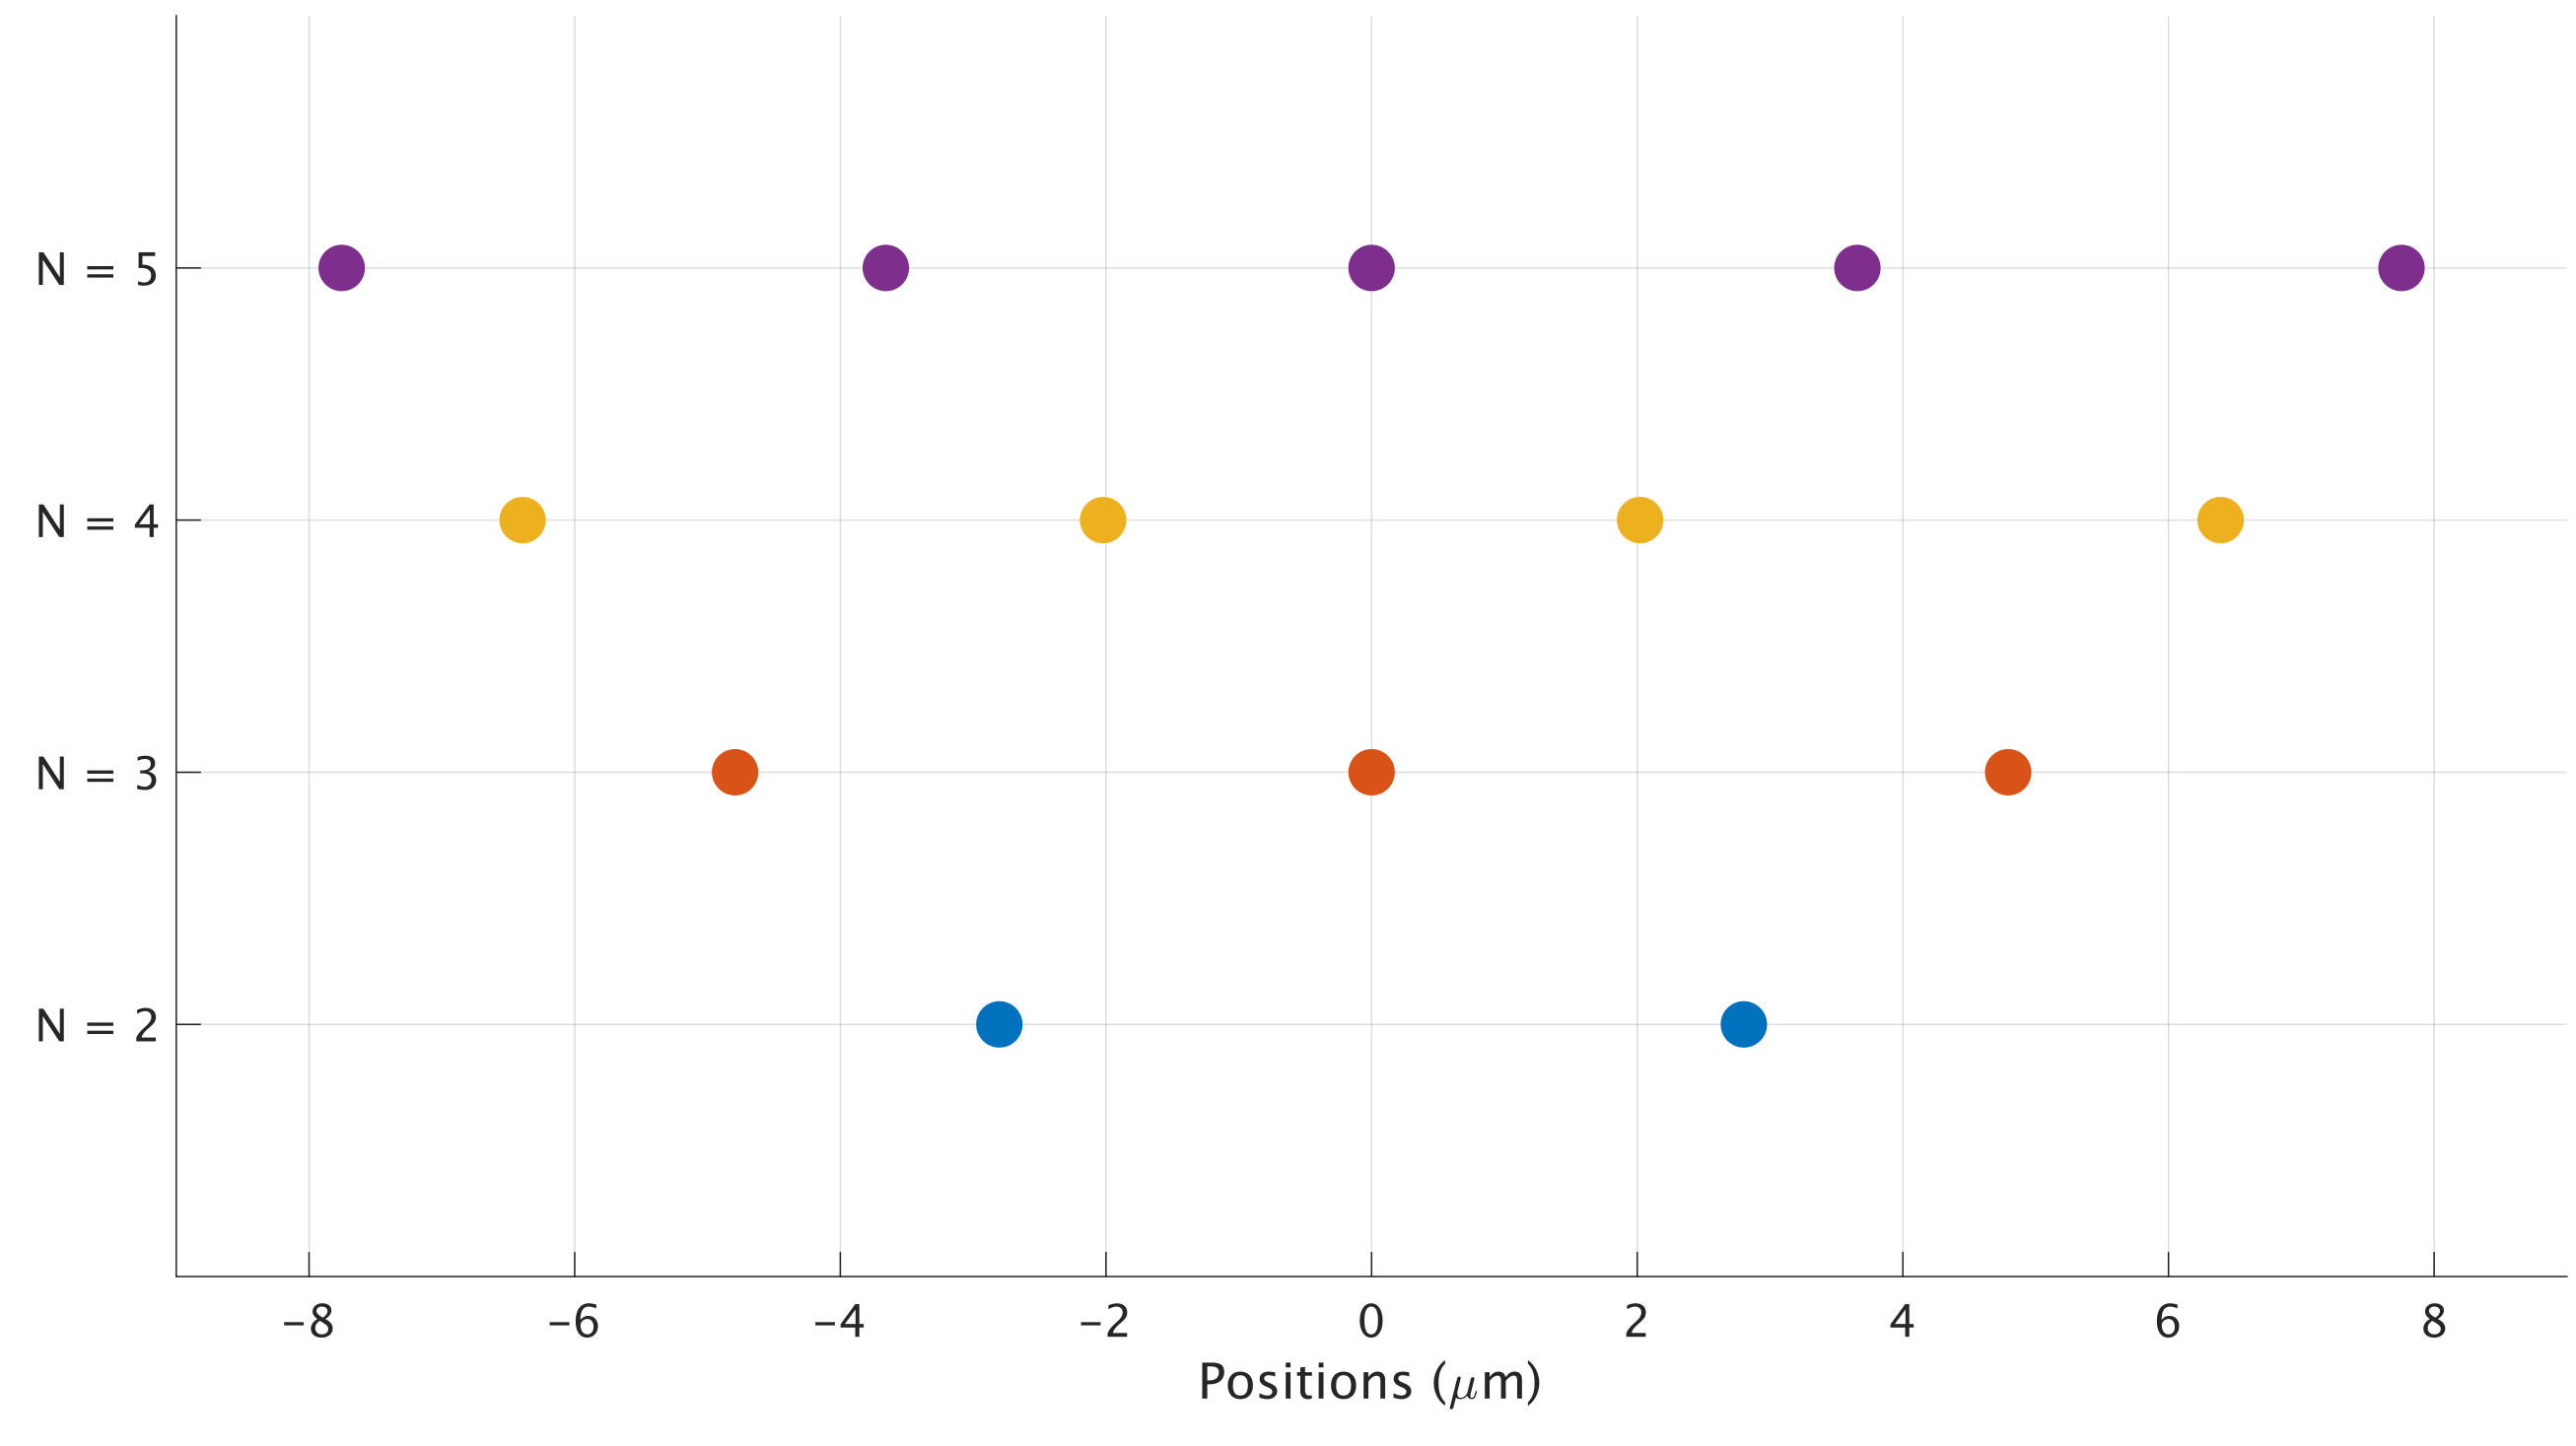
\includegraphics[width = \textwidth]{positions_ions2}
\caption{Ions position for different number $N$ of ions in the trap. Confinement is $\omega_z = 2\pi\times 1$ MHz.}
\label{positions_ions}
\end{figure}
%
%
% \begin{figure}[H]
% \centering
% 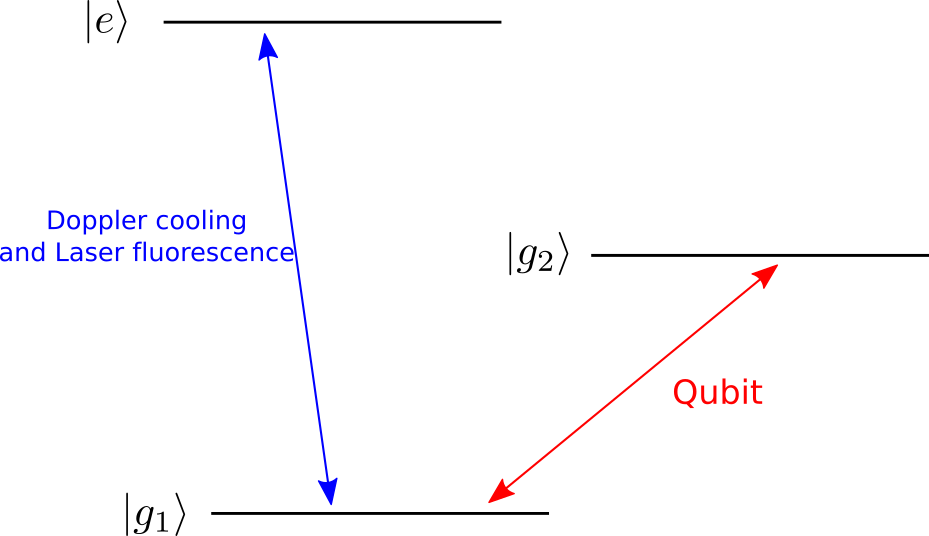
\includegraphics[width = .6\textwidth]{threelevelatom}
% \caption{$\Lambda$ type scheme. Two ground states $\ket{g_1}$ and $\ket{g_2}$ are stable or metastable, while the excited level $\ket{e}$ is short lived. Qubit is encoded in the two ground states while laser fluorescence and laser cooling is done on the $\ket{g_1}\to \ket{e}$ transition. The transition $\ket{e}\to \ket{g_2}$ is repumped to avoid for the electron to be stuck in $g_2$.}
% \label{threelevel}
% \end{figure}
\subsection{Doppler cooling}
\label{sec:doppler_cooling}

Coherent manipulation of ions requires cooling them to reach at least the Lamb Dicke regime \cite{Wineland1998}, where the extent of the ion wave packet is much smaller than the optical wavelengths of the lasers. The idea comes from neutral atoms \cite{1975OptCo..13...68H} and can be applied to ions as well: a laser interacts with a particular transition, exchanging a photon and therefore giving a momentum kick $\Delta p = \hbar \mathbf{k}$ in a particular direction to the ion. The absorbed photon is given back through spontaneous emission in a random direction, giving another kick to the ion. Over many cycles of absorption and emission, the random kick due to emission will average to zero, while the kick given by the laser will accumulate slowing down and cooling the ion in the direction of the laser. \\
The mathematical model is a 2-level atom interacting with a laser (Rabi frequency $\Omega$, and detuning $\Delta$) as described in Section \ref{laserioninteractions}. Spontaneous emission is included with the master equation \eqref{masterequation}, where $\Gamma$ is the spontaneous emission rate. The master equation can be explicitly written for every component of the density matrix $\rho_{ij}$, in the rotating frame they are called optical Bloch equations \cite{foot}. Following the approach of \cite{gabriel}, the system reaches equilibrium when $\rho_{ee}(t\to \infty)$:
% \begin{equation}
% \label{rhoee}
% \frac{d\rho_{ee}}{dt} = -i\frac{\Omega}{2}(\rho_{eg} - \rho_{ge}) - \Gamma \rho_{ee}
% \end{equation}
% \begin{equation}
% \frac{d\rho_{gg}}{dt} = i\frac{\Omega}{2}(\rho_{eg} - \rho_{ge}) + \Gamma \rho_{ee}
% \end{equation}
% \begin{equation}
% \frac{d\rho_{ge}}{dt} = -\left(\frac{\Gamma}{2}+i\Delta\right)\rho_{ge} -i\frac{\Omega}{2}(\rho_{ee} - \rho_{gg})
% \end{equation}
% \begin{equation}
% \frac{d\rho_{eg}}{dt} = -\left(\frac{\Gamma}{2}-i\Delta\right)\rho_{eg}+i\frac{\Omega}{2}(\rho_{ee} - \rho_{gg})
% \end{equation}
\begin{equation}
\rho_{ee}(t\to \infty) = \frac{\Omega^2/\Gamma^2}{1 + \left(2\frac{\Delta -\mathbf{k}\cdot \mathbf{v}}{\Gamma}\right)^2 + 2\frac{\Omega^2}{\Gamma^2}}
\end{equation}
where $\mathbf{v}$ the velocity of the ions. The force exerted on the ions, due to the radiative pressure, is proportional $\rho_{ee}$ as
\begin{equation}
F = \hbar k \Gamma \rho_{ee} \simeq F_0 + \frac{dF}{dv}v = \hbar k \Gamma\frac{\Omega^2}{\Gamma^2 +4\Delta^2} + F_0 \frac{8k\Delta}{\Gamma^2 + 4\Delta^2}v
\end{equation}
where we assumed low velocities $v \simeq 0$ and thus linearized the equation. The effect of the constant term in the force is just to displace the ion from its central position. Instead, the linear term acts as a viscous friction that cools the ions with a rate of $\dot{E}_c = \braket{Fv}$.
If on one side spontaneous emission allows for Doppler cooling, it also sets the lower limit. The small fluctuations in the Brownian motion leads to diffusion which heats the ion at a rate of
\begin{equation}
\dot{E}_h = \frac{1}{m}\frac{d}{dt}\braket{p^2} =  \frac{1}{m}(\hbar k)^2 \Gamma \braket{\rho_{ee}(v)}.
\end{equation}
At equilibrium, the heating rate equals the cooling rate giving the lowest temperature achievable
\begin{equation}
\dot{E}_h + \dot{E}_c = 0  \implies k_B T = -\frac{\hbar \Gamma}{4}\left(\frac{\Gamma}{2\Delta} +\frac{2\Delta}{\Gamma}\right).
\end{equation}
From here it is clear that by choosing the appropriated detuning, it is possible to reach the lowest temperature
\begin{equation}
T_{min} = \frac{\hbar \Gamma}{2k_{B}}, \qquad \text{for} \quad \Delta = -\frac{\Gamma}{2}.
\end{equation}
At this temperature, the average phonon number is $\braket{\hat{n}} = \Gamma /2\omega_z$ \cite{Eschner:03}.\\
As an example, calcium ions confined in a trap with $\omega_z = 2\pi\times 1$ MHz, can be cooled using the transition $\ket{\text{S}_{1/2}}\to \ket{\text{P}_{1/2}}$ ($\Gamma = 2\pi\times 20.8$ MHz), the 2-level atom model in this case gives a good estimation, even though calcium has more levels. The Doppler temperature is $T_{min} \sim 500\,\mu$K, and the corresponding average phonon number is $\braket{\hat{n}} = 10.4$. The wavefunction extend for this phonon number can be found as the standard deviation of the operator $\hat{z}$ for the vibrational state $\ket{n}$, creation and annihilation operator algebra gives
\begin{equation}
\sigma_z = \sqrt{\braket{\hat{z}^2}} = \sqrt{\frac{\hbar}{2m\omega_z}(1+2\braket{\hat{n}})} \simeq 52\,\text{nm}.
\end{equation}
An ion cooled with Doppler cooling therefore has a spatial dimension still much smaller than the ion separations.\\
To further decrease $\braket{\hat{n}}$, sideband cooling can be used \cite{Eschner:03}, here particular sideband transitions are excited to reduce the phonon number of the ions inside the trap. However in the experiments of this thesis, only Doppler cooling has been performed.
\section{Laser beam}
\subsection{Gaussian beams}
\label{sec_diffraction}
Typically, lasers emit light in the shape of Gaussian beams, so it is import to understand what Gaussian beams are and their characteristics. In this chapter we will take a closer look into such beams and introduce important quantities to characterize a Gaussian beam. \\
From a theoretical point of view, Gaussian beams are a solution of the Helmholtz equation $(\nabla^2 + k^2)U(\mathbf{r}) = 0$, with $k$ being the wavevector, and $U(\mathbf{r})$ the complex electric field. If we can consider a wave propagating in the $z$ direction, we can write it as \cite{saleh}:
\begin{equation}
\label{gaussianbeams}
U(\mathbf{r}) = A_0 \frac{W_0}{W(z)}\exp\left\{-\frac{x^2+y^2}{W^2(z)}\right\}\exp\left\{-ikz-ik\frac{x^2+y^2}{2R(z)}+i\arctan(z/z_0)\right\}.
\end{equation}
Where $A_0$ is an amplitude, $W(z)$ the width, $R(z)$ the curvature radius, and $z_0$ the Rayleigh range. The intensity can be calculated by taking the square of the complex amplitude
\begin{equation}
\label{beamintensity}
I(\mathbf{r}) = |U(\mathbf{r})|^2 = I_0 \left(\frac{W_0}{W(z)}\right)^2 \exp\left\{-\frac{2x^2 + 2y^2}{W^2(z)}\right\}  \qquad I_0 = |A_0|^2.
\end{equation}
For a fixed $z$, i.e. the sections in the $x-y$ plane are shaped as a two dimensional Gaussian distribution. For simplicity, let us take the profile for a fixed $z$ and $y=0$:
\begin{equation}
I(x,y=0,z) = \widetilde{A}(z) \exp\left\{\frac{2x^2}{W^2(z)}\right\} \qquad \widetilde{A}(z) = I_0 \left(\frac{W_0}{W(z)}\right)^2  .
\end{equation}
In Figure \ref{gauss}, the $x$ cross section is depicted for this intensity profile normalized in amplitude. Parameters used to measure the width are also displayed and defined in the caption. All of those quantities are equivalent and differ only by a prefactor, so for the rest of the section, we stick to $W(z)$ (point at which $I$ has fallen to $1/e^2 = 13.5\%$) and study its behaviour.
\begin{figure}
\centering
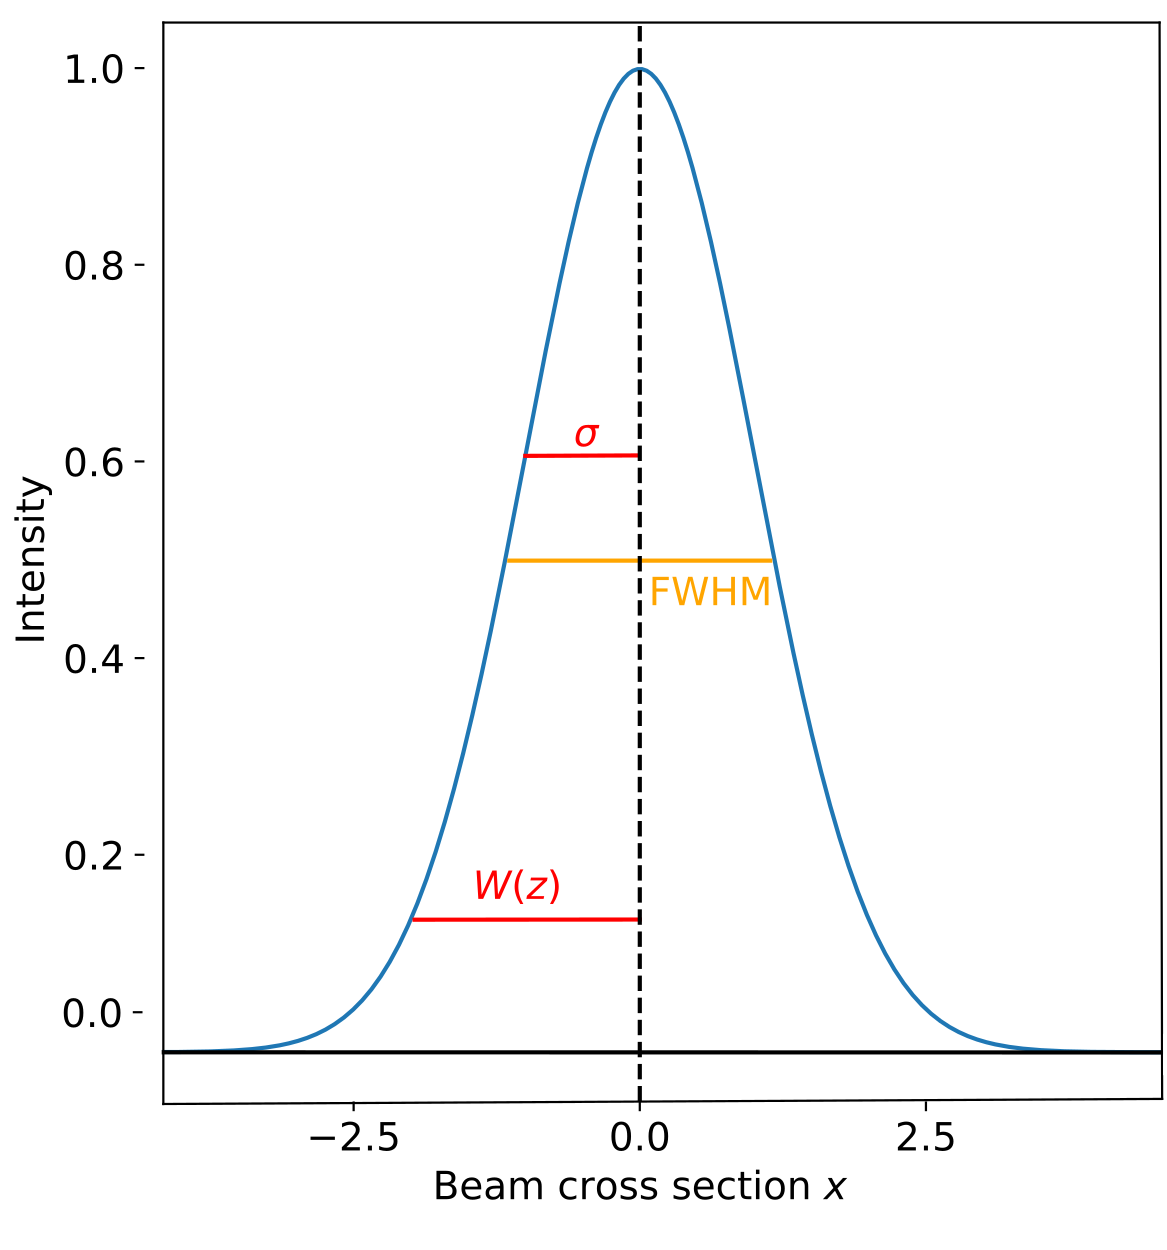
\includegraphics[width = .6\textwidth]{gauss2}
\caption{Cross section of the intensity profile of a Gaussian beam $I(x) = e^{-x^2/2\sigma^2}$. The beam is normalized and $\sigma=1$. Graphical representations of used widths are displayed: $W(z)$ is defined as the point at which the intensity $I$ has fallen to $1/e^2 = 13.5\%$ of its maximum value; $\sigma$ is the standard deviation of a Gaussian in the form $Ae^{-\frac{x^2}{2\sigma^2}}$; FWHM is the full width half maximum. Relationships among these quantities are: $W(z) = 2\sigma$, and $W = 0.84\cdot \text{FWHM}$.}
\label{gauss}
\end{figure}
From Helmholtz equation \cite{saleh}, the profile of $W(z)$ as a function of $z$ is found to be
\begin{equation}
\label{waistprofile}
W(z) = W_0 \sqrt{1 + \left(\frac{z}{z_0}\right)^2}\qquad W_0 = \sqrt{\frac{\lambda z_0}{\pi}} \qquad z_0 = \frac{\pi W_0^2}{\lambda}.
\end{equation}
$\lambda$ is the wavelength, and $W_0$ and $z_0$ are respectively the waist of the beam and the Rayleigh range discussed below. A plot of \eqref{waistprofile} is presented in Figure \eqref{gaussprofile}:
the width $W(z)$ assumes its minimum value $W_0$ at $z=0$, this spot is called focus and its width $W_0$ is the waist of the beam. The Rayleigh range $z_0$ gives an idea of how quickly the beam is expanding. Mathematically $z_0$ is the distance between the focus and the point where the width is $W(z) = \sqrt{2}W_0$.
For $z \gg z_0$, the beam profile diverges almost linearly with an angle given by $\theta = W_0/z_0$, which means the smaller the focus, the greater it diverges.\\
This property will become important later in the work, because it provides one limit on the waist of the beam in our experimental system. In fact, the optical aperture of the trap is limited by some electrodes, and a beam that diverges too rapidly can potentially clip on one electrode causing aberrations and scattered light in the trap.\\
A Gaussian beam can be reshaped using optical elements.
\begin{figure}
\centering
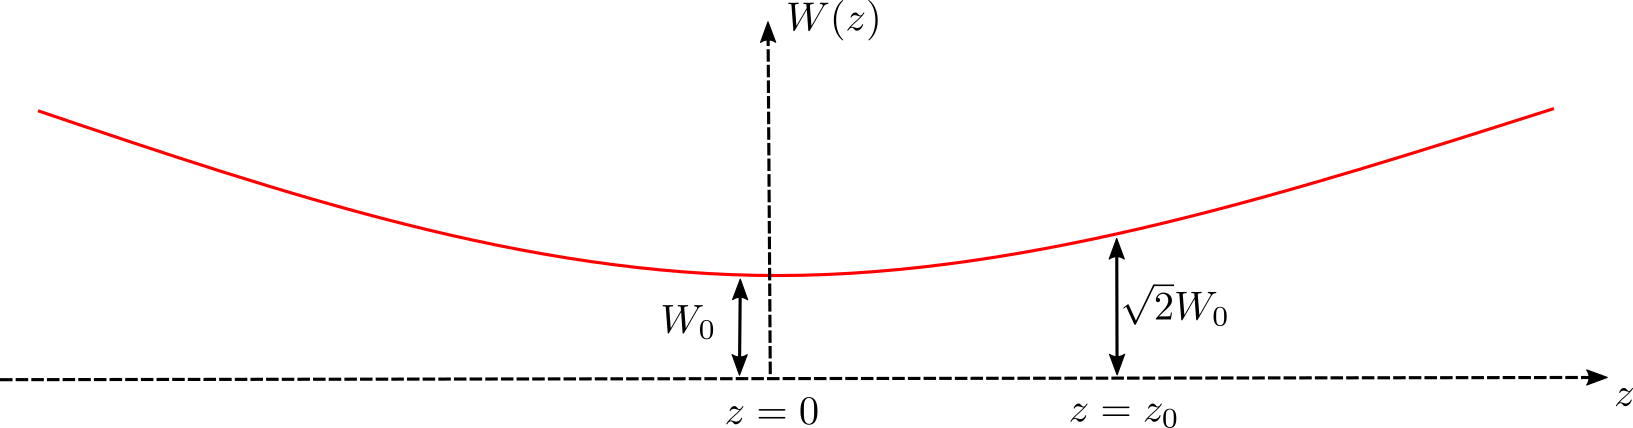
\includegraphics[width = \textwidth]{gaussprofile}
\caption{Width profile of a Gaussian beam along the direction of travel of the beam, equation \eqref{waistprofile}. The beam is focused at the position $z = 0$, here it assumes the minimum width $W_0$, also referred to as the waist. $z_0$ is the Rayleigh range where the width is $\sqrt{2}W_0$}
\label{gaussprofile}
\end{figure}
In order to study such reshaping, let us consider a thin spherical lens with focal length $f$, and radius of curvature $R_l$ placed at position $z$. The effect of the lens on the beam is to give an extra phase factor $k(x^2 + y^2)/2f$ to equation \eqref{gaussianbeams} \cite{beamparameters}. We can match the phase of the incoming and emerging waves, which have respectively radius of curvature $R$, and $R'$, this results in
\begin{equation}
\frac{1}{R'} = \frac{1}{R} - \frac{1}{f}.
\end{equation}
The effect of the lens is to change the radius of curvature to $R'$. Moreover, the width of the beam at the lens is not altered $W=W'$. Using these last two facts, we can determine all the parameters of the outgoing wave. The most important for us is the new waist $W_0'$
\begin{equation}
W_0' = MW_0 \qquad M = \frac{M_r}{\sqrt{1+r^2}}.
\end{equation}
Where $M_r = \left|\frac{f}{z-f}\right|$, and $r = \frac{z_0}{z-f}$. $M$ is the magnification factor which provides an easy way to describe the change of the beam. For a better understanding of this last result, let us consider a less general example. We place the lens at the focus $z=0$, and have a collimated beam $z_0 \to +\infty $. In this case the new waist is
\begin{equation}
\label{eq:newwaist}
W_0' = \frac{W_0}{\sqrt{1 + (z_0/f)^2}} \simeq W_0\frac{f}{z_0} = \frac{\lambda f}{\pi W_0}
\end{equation}
where the approximation comes from taking $z_0\gg f$. There are three parameters we can act on to achieve the smallest waist. A shorter wavelength $\lambda$ results in a smaller waist. Similarly, a lens with a shorter focal length $f$ reduces the waist. Finally, a broader incoming beam, i.e. larger $W_0$, also narrows the waist. Given a certain lens and a wavelength, the smallest waist is obtained with the largest incoming beam which is limited by the lens diameter $D$, i.e. $2W_0 = D$. In this case, equation \ref{eq:newwaist} becomes
\begin{equation}
\label{eq:difflimited}
W_0' = \frac{2\lambda}{\pi} \frac{f}{D}.
\end{equation}
If the size of the collimated beam is further increased, the lens becomes a finite size aperture and diffraction effects will appear at the image plane. In general, an optical system (in our example a single lens) that is limited in the sense of \eqref{eq:difflimited} is said to be diffraction limited \cite{diocane}.
%An a numerical example, the objective used in this thesis setup has an aperture of 40 mm, focal length of 54 mm, therefore for a wavelength of $\lambda = 393$ nm the best achievable waist is $1.02\,\mu$m.

\subsection{Beam stearing via Acousto-optical Deflectors}
\label{theory_AOD}
An acousto-optical deflector (AOD) is a common device that can change the propagation direction of a laser beam, typically on the few microsecond timescale. In this work we use an AOD to change which ion is illuminated by a single-ion focused laser. The working principle of an AOD is based on the Acousto-optical effect. A piezo is used to create acoustic waves that propagate through a crystal. The waves modify the crystal refractive index, creating a periodic optical grating that can deflect light travelling through it.  \\
Following the approach of \cite{saleh} to model the device, let us consider a rectangular crystal like in Figure \ref{AOD}. The acoustic wave creates a sinusoidal pattern with frequency $\Omega_s$ and wavenumber $q$, for the refractive index $n(x,t)$
\begin{equation}
n(x,t) = n - \Delta n_0 \cos \left(\Omega_s t - qx \right),
\end{equation}
where $n$ is the refractive index of the unperturbed medium, $\Delta n_0$ is the amplitude of the perturbation. $\Delta n_0$ is proportional to the square root of the sound intensity.
\begin{figure}
\centering
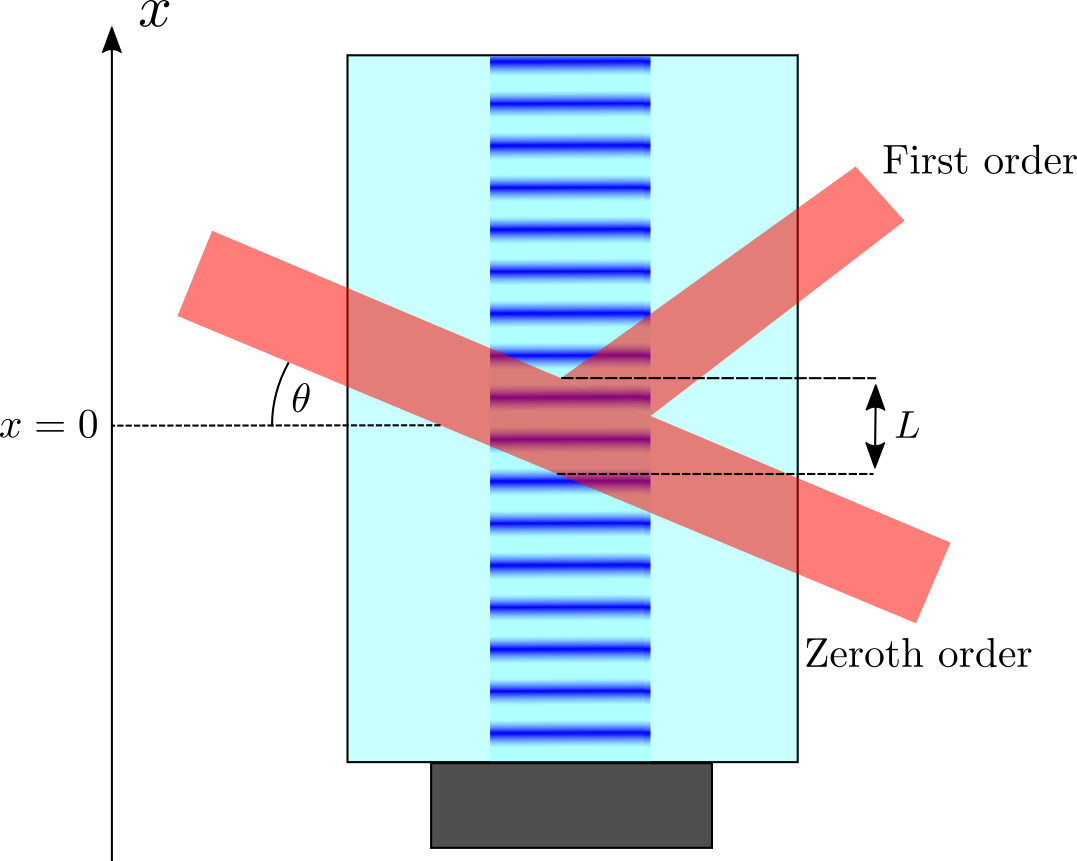
\includegraphics[width = .5\textwidth]{aod2}
\caption{Simple model of an AOD. In black at the bottom a black piezo that generates acoustic waves through the light blue crystal. In red, a collimated beam of light enters in the crystal with an angle $\theta$ and gets partially deflected due to the interaction with the effective optical grating created by the acoustic waves.}
\label{AOD}
\end{figure}
The complex amplitude of the refracted light $r$ can be calculated by dividing the crystal in thin layers with thickness small compared to the acoustic wavelength. Therefore, we assume that the refractive index $n(x)$ is approximately constant across the layer. The total refraction is given by all the contributions $\frac{dr}{dx}$ of every layer, we can therefore integrate in the $x$ direction over the length $L$ as follow:
\begin{equation}
r = \int_{L/2}^{L/2} e^{i2kx \sin\theta} \frac{dr}{dx} \,dx
\end{equation}
The included phase takes into consideration the different phase of the input laser beam when different layers are met. The integral can be solved with a change of variable
\begin{equation}
\frac{dr}{dx} = \frac{dr}{dn}\frac{dn}{dx} = \frac{dr}{dn} q \Delta n_0 \sin \left(\Omega_s t - qx \right),
\end{equation}
The sine function can be written as exponential and now the integral contains only exponential functions which are trivial to calculate. At the end we obtain two contributions for the refracted wave $r$:
\begin{equation}
\label{mainAOD}
r = r_+ + r_- \qquad r_\pm = \pm i r_0 \text{sinc} \left[(2k\sin(\theta) \mp q)\frac{L}{2\pi} \right]e^{\pm i\Omega_s t}
\end{equation}
These two terms are the plus and minus first order diffraction, an acousto-optical device can be operated symmetrically entering either with a positive angle or with a negative one. Since the maths and the physics is the same, we will focus only on the positive term, called upshifted Bragg diffraction. The sinc function peaks sharply when its argument is 0, i.e. at $2k\sin\theta = q$, and then quickly decreases as the angle is changed. Hence, the input beam must enter with a particular angle $\theta_B$ in order to diffract with maximum efficiency. The condition to be satisfied is called the Bragg condition, and can be written as a function of the optical ($\lambda$) and acoustic ($\Lambda_s$) wavelengths as
\begin{equation}
\label{braggcondition}
\sin \theta_B  = \frac{\lambda}{2 \Lambda_s} \qquad \Lambda_s = \frac{2\pi}{q}.
\end{equation}
If the condition is not perfectly matched, some light will not be diffracted and will be transmitted unaltered through the device.
The ratio of the transmitted and diffracted light is called diffraction efficiency and gives an idea of how well an acousto-optical device is performing.\\
From equation \eqref{mainAOD} we can notice that an extra phase factor proportional to $\Omega_s t$ is added to the reflected wave. Thus, if the incoming wave is oscillating at $\propto e^{i\omega t}$, the diffracted wave will oscillate as $\propto r_{+}e^{i\omega t} \implies \propto e^{i(\omega + \Omega_s )t}$. The frequency of the diffracted optical wave $\omega_r$ is therefore shifted by the frequency of the acoustic vibration as
\begin{equation}
\label{eq:aodshift}
\omega_r  =  \omega + \Omega_s.
\end{equation}
The acousto-optical effect described above is common to different devices optimized for specific tasks. Two of the most commons devices are Acousto-optical Deflectors (AOD) and Acousto-optical Modulators (AOM). The idea of the latter is to shift the frequency of a laser using equation \eqref{eq:aodshift}. Deflectors instead exploit the fact that the deflection angle $\theta$ changes linearly as a function of the acoustic frequency $\Omega_s$. Assuming that the angle $\theta$ is small enough to approximate $\sin\theta \sim \theta$, the Bragg condition can be written as
\begin{equation}
\theta \simeq \frac{\lambda}{2 v_s}f,
\end{equation}
where $v_s$ is the speed of sound and $f$ the frequency of the acoustic wave. We can already see that if we change the frequency $f$, the deflection angle $\theta$ changes proportionally. Although the Bragg condition \eqref{braggcondition} is not satisfied anymore, we can work with small enough angles that the diffraction efficiency remains above a certain threshold. The bandwidth $B$ specifies the range of frequencies over which deflectors work.\\
AOMs and AODs differ by the relative divergence of the optical and acoustic beam \cite{handbookoptics}, moreover for AODs, speed and the number of resolvable spots are more important, while for AOM's the optimization is on modulation bandwidth. These different priorities in building the devices influence
the choice of the crystal and acoustic mode, for instance, a slow acoustic velocity and shear mode are preferred in AODs \cite{handbookoptics}.

\section{Basic model of key experiments}
The aim of this thesis is to perform two experiments with ions: qubit manipulation, and photon generation. In addition to test these two functionalities, the experiments are also designed to asses the performance of the addressing system as discussed below. In both cases a string of 3-4 ions is loaded in the trap, the addressed Raman laser is focused on a single ion and experiments are carried out.

\subsection{Addressed qubit manipulation}
\label{sec:expqubit}
\begin{figure}
\centering
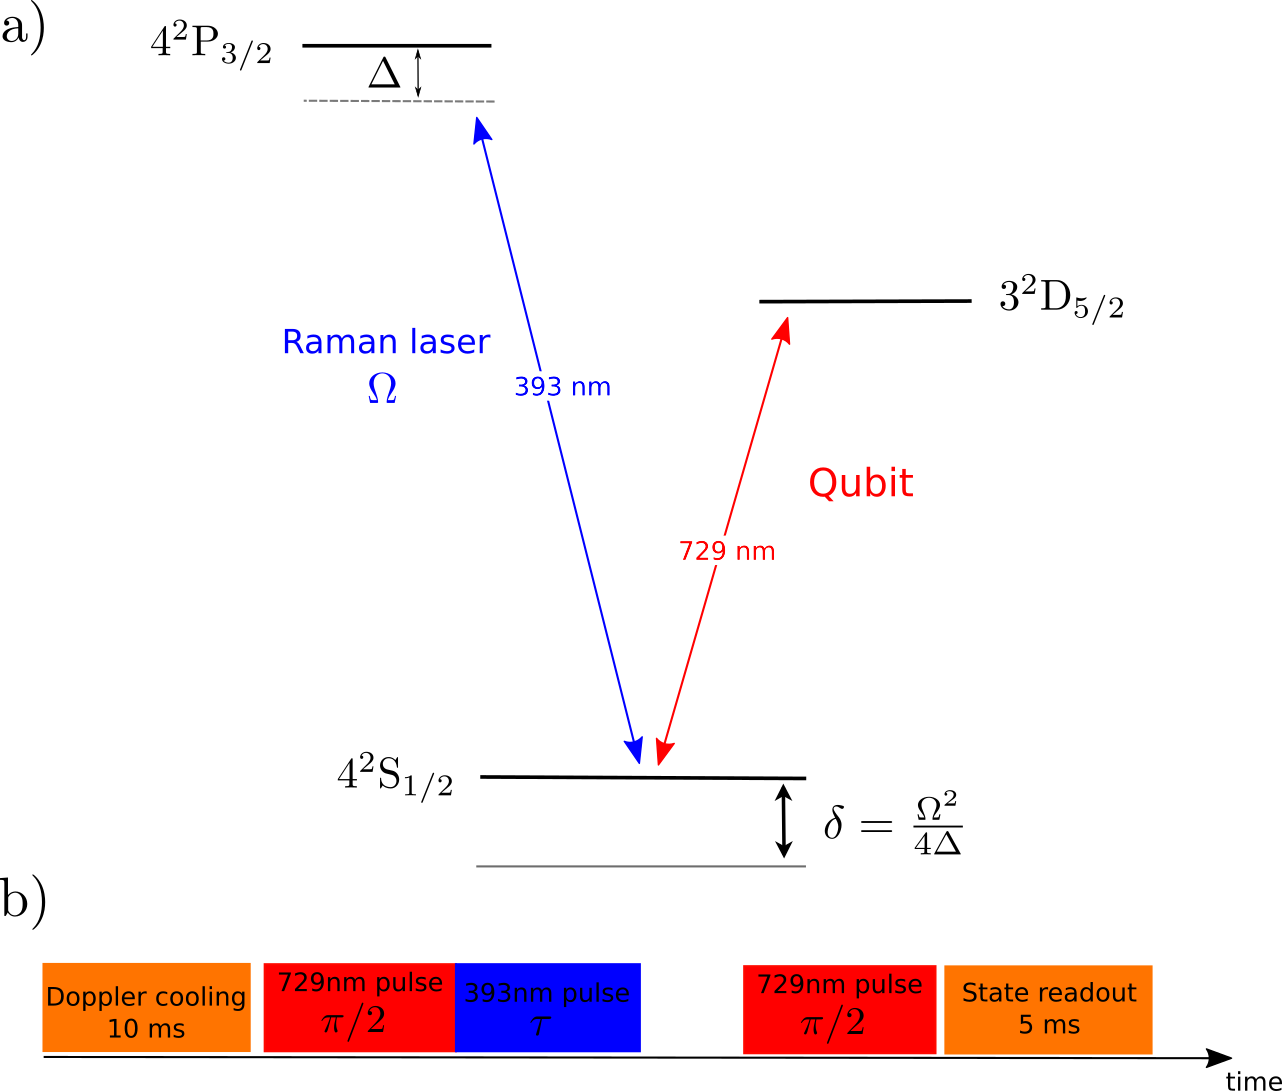
\includegraphics[width=.7\textwidth]{exp1}
\caption{a) Relevant levels for the experiment, the qubit is encoded in the 729 nm transition, the 393 nm laser is used to shift the $\ket{S}$ level via AC Stark shift b) Experiment pulse sequence, Doppler cooling and state readout are described in Section \ref{sec:expparameters}. The time $\tau$ had a variable length.}
\label{sequence}
\end{figure}
As we have seen, ions can be used to encode and process quantum information. As highlighted in Figure \ref{sequence}, the qubit is encoded in the $\ket{S} \to \ket{D}$ transition. The 393nm transition from $\ket{S}\to \ket{P}$ can be used to induce a phase shift on the ground state of the qubit $\ket{S}$. In the off resonant regime, the laser induces a Stark shift $\delta = \Omega^2/4\Delta$ without actually exciting the state. As discussed in Section \ref{sec:dissipation}, in order for this to happen, we should have $\delta \gg \Gamma_{eff}$. Therefore in the experiment we decided to set the detuning such that the ratio between the Stark shift and the spontaneous scattering rate is 100
\begin{equation}
\frac{\delta}{\Gamma_{eff}} = \frac{2\Delta}{\Gamma} \sim 100 \implies \Delta \sim 3\,\text{GHz}.
\end{equation}
Furthermore, ions can be used as sensitive tools for beam profiling, the addressed manipulation changes only the qubit state of a single ion. Hence, by measuring the state of all ions, and scanning the beam across the ions string, a beam profile can be obtained. In a single experiment we can therefore characterize the beam and demonstrate qubit manipulation.
The experiment consists of Ramsey interferometry, already performed in the past to measure AC Stark shift \cite{starkshift}.
In summary, the idea is to send a resonant $\pi/2$ pulse at 729 nm, which brings the qubit state to a superposition $\ket{S}+\ket{D}$, here another in phase resonant $\pi/2$ pulse at 729 nm would bring the final state to the excited level $\ket{D}$. However, if between the two 729 nm pulses, AC stark shift is induced by a pulse of 393 nm light, an additional phase is added to the superposition $\ket{S}+\ket{D}$, and the final state after the second 729 nm pulse will depend on the shift induced by the 393nm laser. The phase of the second 729 nm pulse can also be varied. By calculating the final probability $P_D$ it is possible to infer the Rabi frequency of the 393 nm light. Rigorous mathematic can be done with matrices \eqref{laserpulse} here called $U_{729}$ and \eqref{acstarkrotation}, referred to as $U_{393}$. After the three pulse sequence the final state is
\begin{equation}
\begin{split}
\ket{\psi_f} &= U_{729}(\pi,\phi)U_{393}(\delta)U_{729}(\pi,0)\ket{S} \\
&= \frac{1}{2}\left(e^{-i\frac{\delta}{2}\tau}-e^{-i\phi}\right)\ket{S}-\frac{i}{2}\left(1 + e^{-i\frac{\delta}{2}\tau} e^{-i\phi}\right)\ket{D}
\end{split}
\end{equation}
where $\delta = \Omega^2/4\Delta$ is the Stark shift, and $\Omega$ is the Rabi frequency of the 393nm light that we want to measure. The final probability is then
\begin{equation}
\label{stupidequation}
P_D = \cos^2\left(2\phi + 2\frac{\delta \tau}{2}\right) = \cos^2\left(2\phi + \frac{\Omega^2 \tau}{4\Delta}\right).
\end{equation}
As we can see, the final signal depends on the phase of the second 729nm pulse $\phi$ and on the Stark shift induced by the 393nm laser. To get $\Omega^2$ a simple formula inversion can be done
\begin{equation}
\label{eq:ptointensity}
\Omega^2 = \left[\text{arccos}\left(\sqrt{P_D}\right)-2\phi \right].
\end{equation}
The phase $\phi$ can be set experimentally and all constants have been dropped as the data will be normalized. The experiment sequence is in Figure \ref{sequence}. For every sequence, a stage of Doppler Cooling at the beginning is included and at the end of the pulses state readout with single-ion resolving camera is performed. For each 393 nm pulse length $\tau$ the sequence is repeated $N=50$ times to obtain and estimate the electronic excitation probability.

\subsection{Addressed photon generation}
\label{sec:expphoton}
\begin{figure}
\centering
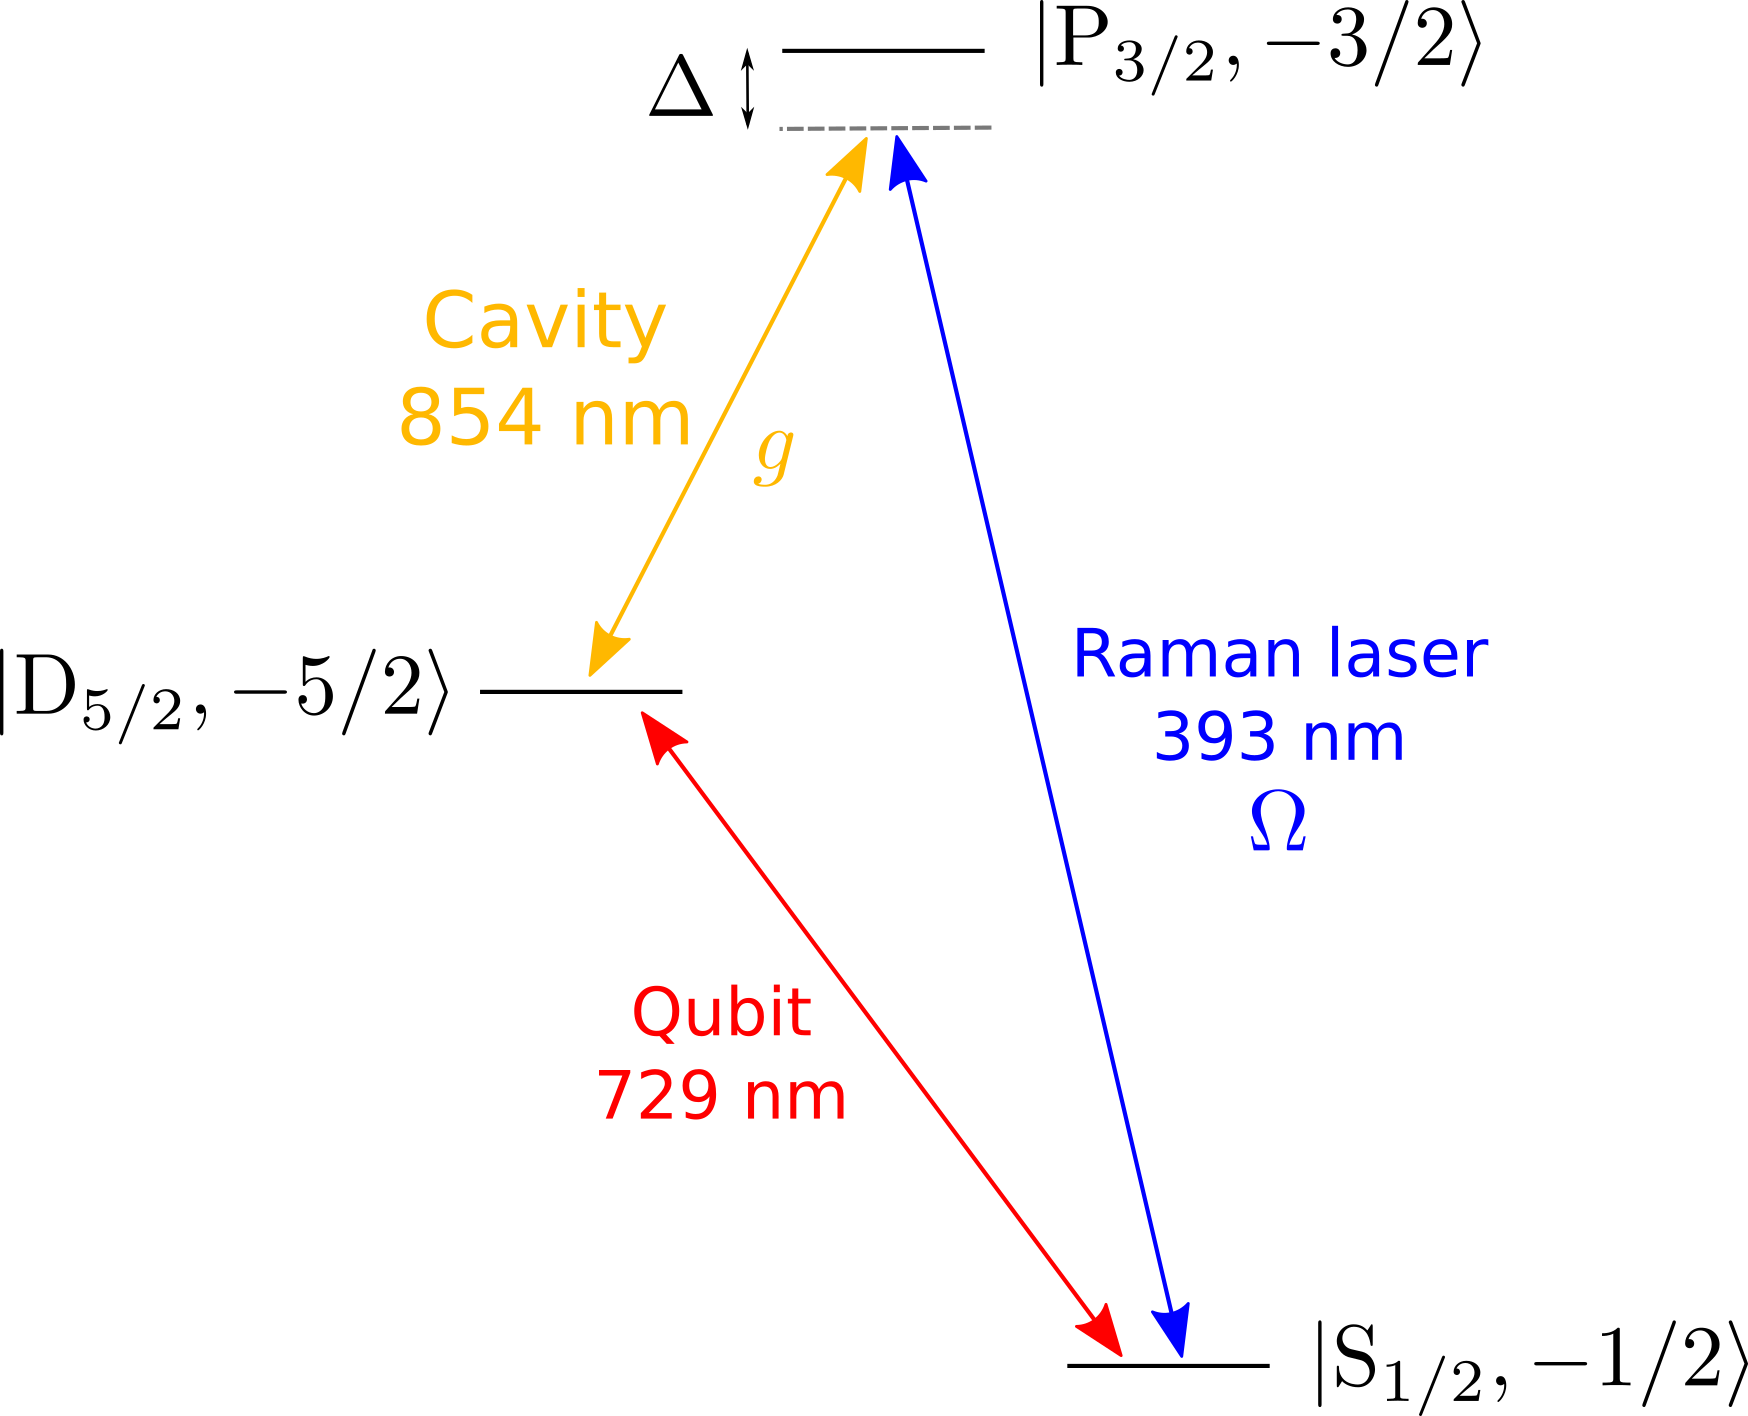
\includegraphics[width=.5\textwidth]{exp2}
\caption{Scheme of the Raman process used to generate photons, via a cavity enhanced Raman process (Section \ref{sec:ramanprocess}). The electron in the $\ket{S}$ state is excited to the $\ket{D}$ level by absorbing a 393 nm photon and emitting a 854 nm photon in the cavity.}
\label{img:sec2}
\end{figure}
The second experiment consists of generating photons from one single ion out of a string, using the cavity-mediated Raman process described in Section \ref{sec:ramanprocess}. In figure \ref{img:sec2} the relevant levels are depicted. First, the ion is positioned in a maximum of the cavity vacuum electric field such that the coupling atom-cavity $g$ is maximized. Second, a 393 nm laser pulse triggers the generation of a photon into the cavity through the Raman process. The detunings of the cavity and laser pulse must be equal, moreover the detuning should be large enough to adiabatically eliminate the $P$ state and avoid spontaneous scattering. As seen in Section \ref{sec:ramanprocess}, this is ensured by a detuning of $\Delta \sim 400$ MHz.
In this process the population of the state $\ket{S}$ is coherently transferred to the $\ket{D}$ state by absorbing a 393 nm photon and emitting a 854 nm photon in the cavity, the photon then exits from the cavity. The states involved in the dynamics are
\begin{equation}
\ket{\text{S}_{1/2},-1/2} \to \ket{\text{P}_{3/2},-1/2} \to \ket{\text{D}_{5/2},-3/2}.
\end{equation}
Note that the effective Rabi frequency of the population transfer is proportional to the laser drive Rabi frequency $\propto \Omega$ as seen in equation \eqref{omegaeff}. On the contrary, AC Stark shift depends on the Intensity $\propto \Omega^2$. Therefore, the addressing error in the two experiments are different. After the excitation and photo emission, state detection on all ions is performed, this gives the possibility to check if other ions have been undesirably addressed.


%Existing experimental setup chapter
% !TEX root = main.tex

\chapter{Existing experimental system}
The work developed in this thesis lies on top of an existing experiment. In this chapter we are going to describe the essential parts of the already existing setup on top of which the addressing system has been build. Calcium-40 ions are used in the experiment, the implementation of several techniques for
trapping and manipulating these ions are discussed. Furthermore, the addressing setup utilizes 393nm light, the laser emitting this light was already installed and used, thus that setup is presented. The experiment can be controlled remotely via computers, an overview of how it is implemented and how it works is also given.

\section{Ion trap and key techniques}
\subsection{Calcium Ions}
In choosing the appropriate ion to trap, one looks first of all for simplicity, which means choosing an element with one single electron in the most outer orbital.
This fact limits the choice to the second group of the periodic table, many of these elements has been successfully trapped: beryllium [], barium [], strontium [], and calcium [].
The latter has been chosen for this experiment, as calcium has transitions easily accessible with commercial diode and titanium-sapphire lasers. The most abundand isotope of calcium is calcium-40, which is a common choice, but not the only one []. Nevertheless, $^{40}\text{Ca}^+$ ions were our choice. In figure \ref{calciumscheme} the level scheme of the only electron in the outer shell is presented. A single ground state is present $\text{S}_{1/2}$ with no hyperfine structure as $^{40}\text{Ca}^+$ does not posses a nuclear spin. There are two short lived excited states ($\sim 7$ ns): $\text{P}_{1/2}$, and $\text{P}_{3/2}$ which are accessible with dipole transitions. These states have different decay channel, for $\text{P}_{1/2}$
the branching ratios are $6\%$ to $\text{D}_{3/2}$, and $94\%$ back to the ground state. For  $\text{P}_{3/2}$ there is a probability of $5.3\%$ to decay to   $\text{D}_{5/2}$, $0.6\%$ to go to  $\text{D}_{3/2}$ and $94\%$ to return to  $\text{S}_{1/2}$. Due to the short lifetimes of these two states, they are suitable for laser cooling and state detection, while the states $\text{D}_{3/2}$ and $\text{D}_{5/2}$
are metastable ($\sim 1$ s) since accessible with electric quadrupole transition. Since the lifetime of the D states are much greater than typical coherence time, they can encode a stable qubit and manipulated without worrying about dissipative process. Table () summarizes the properties of the states, and details about the different transition.

\begin{tabular}{c c c c c}
 \toprule
    {Transition} & {wavelength (nm)} & {Decay rate $\Gamma$} & {Type} & {Use} \\ \midrule
   16.128 & 1.402 & 1.373 & -146.6 & -137.6 \\
     3.442  & 0.299 & 0.343 & 133.2  & 152.4  \\
     1.826  & 0.159 & 0.119 & 168.5  & -161.1 \\
     0.993  & 0.086 & 0.08  & 25.6   & 90     \\ \midrule
   1.29   & 0.112 & 0.097 & -175.6 & -114.7 \\
     0.483  & 0.042 & 0.063 & 22.3   & 122.5  \\
     0.766  & 0.067 & 0.039 & 141.6  & -122   \\
     0.624  & 0.054 & 0.04  & -35.7  & 90     \\ \midrule
   0.641  & 0.056 & 0.045 & 133.3  & -106.3 \\
     0.45   & 0.039 & 0.034 & -69.4  & 110.9  \\
     0.598  & 0.052 & 0.025 & 92.3   & -109.3 \\ \bottomrule
\end{tabular}

\begin{figure}
\centering
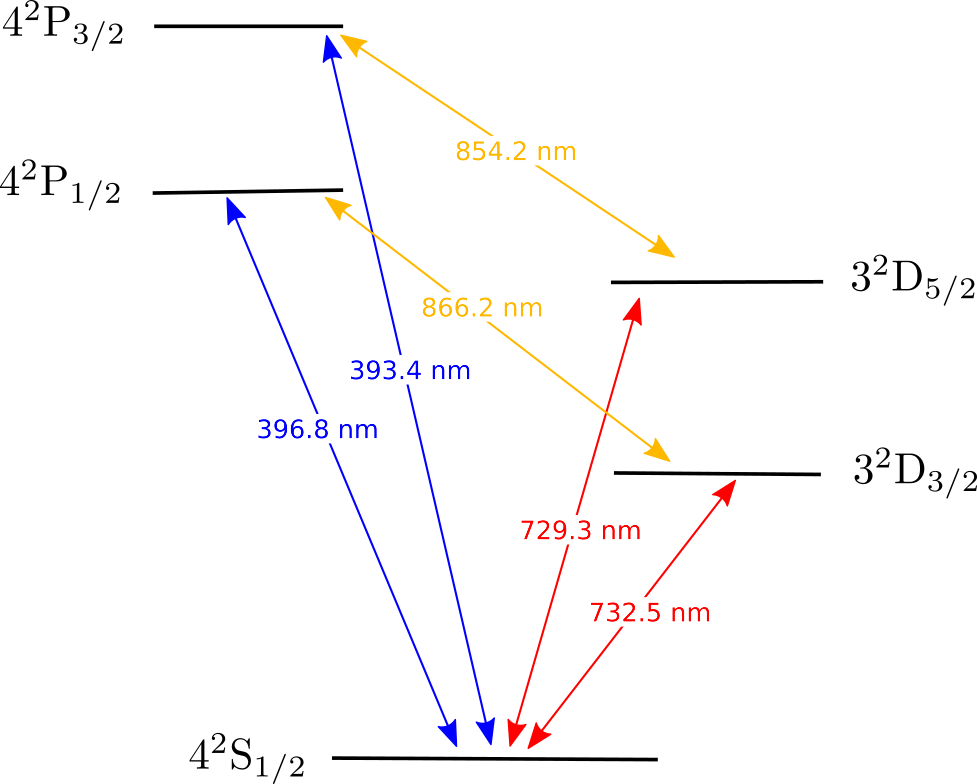
\includegraphics[width = .6 \textwidth]{calciumscheme}
\caption{Level scheme of $^{40}\text{Ca}^+$.}
\label{calciumscheme}
\end{figure}


\subsection{Trapping, cooling, and state readout}
- How this stuff is implemented
\subsection{Photon generations}
- Cavity enhanced Raman transition
\section{393nm laser}
\section{Experiment control}


%Design and simulation
% !TEX root = main.tex
\chapter{Design and simulation of the addressing setup}
The purpose of this thesis work was to design and build the addressing setup for the already existing experiment. In this chapter we discuss the design and the implementation of such setup. The design is a crucial part of the work, there are several requirements that have to be met in order to achieve the proper needed functionality. In the first section, the requirements are presented together with an overview of the design idea. In the setup an objective was already present, and the choice of an AOD was already made. Hence, we discuss this components as given. The rest of the setup was simulated with the software Zemax, which was used to find the optimal optical components and their placement.
\section{Addressing system overview and requirements}
Addressing systems have already been developed and employed in experiments successfully. Different techniques are available: the main idea is to focus a laser beam tighter than ion-ion separation and steer it. In  Innsbruck calcium ions have been addressed in this way, where the steering was achieved with an AOD \cite{addressing}; Beam has also been steered with micro-electromechanical systems (MEMS) mirrors \cite{addressing3}. Another idea is to send a normal beam illuminating all the ions, but hiding those who are not addressed. This was done with Ytterbium atoms where by means of a inhomogeneous magnetic field the transition frequencies were shifted shielding selected ions \cite{addressing2}. \\
Our choice was to implement the already successful idea of Innsbruck with an AOD and improve it. The advantage of AODs is to have a fast switching time in the order of $\mu$s, that is used for fast switching between ions. A problem with the implementation of \cite{addressing} is however the fact that the AOD is placed right before the beam expander, this limits the addressing range, as the beam is likely to clip when it is steered on the edge of the AOD's bandwidth. This is the main problem that the new designed system, here implemented, wanted to address: exploiting the full capabilities of the AOD while maintaining a very tight focus.
Therefore, there are mainly two aspects to keep in mind, the focus spot and the addressing range. However the priority was the focus spot as a large addressing range is not essential.
\begin{figure}[H]
\centering
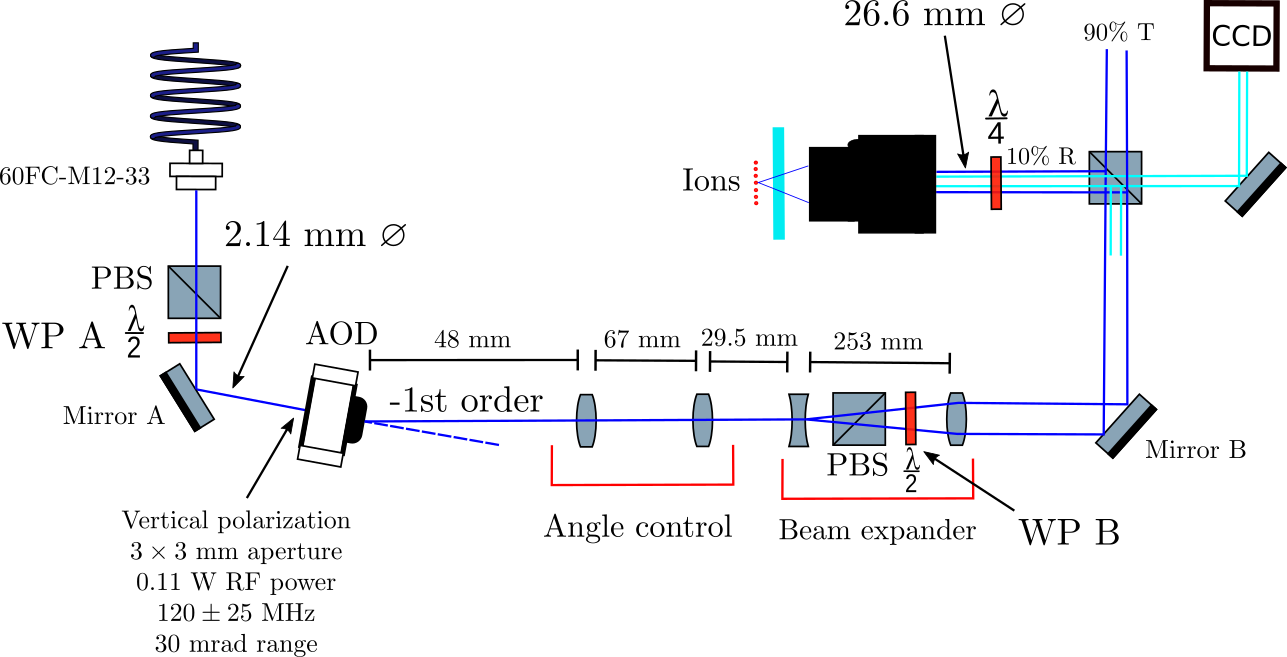
\includegraphics[width=\textwidth]{img/setup}
\caption{Scheme of the setup. Light comes from a fiber, polarization is cleaned, and then sent thorough the AOD. 1st order diffracted light is refocused into a beam expander, where the beam is broadened before being focus by the objective. Light blue lines represents 393 nm light coming from the ions into the imaging setup.}
\label{addressingsetup}
\end{figure}
The addressing setup should be able to address single ions in a string in order to generate single photons out of single ions via the already discussed Raman process. Ion separations, in the case of $^{40}\text{Ca}^+$, has been derived in section \ref{ionstrings}, for a trap frequency of 1 MHz is 5.6 $\mu$m. The setup must therefore be able to focus tightly a laser beam down to 1-2 $\mu$m. As seen in section \ref{sec_diffraction}, a tighter focus can obtained with a shorter wavelength, a bigger lens, or with shorter focal length. The focusing lens, a.k.a the objective, is shared with the imaging setup, and thus it is given, the focal length is therefore a constant in the problem. The wavelength is also a constant, as the Raman process happens only at 393 nm. This gives only one possibility left to tighten the focus, i.e. by making the beam as broad as possible at the objective input surface. Beam expansion can be achieved with a Galilean telescope, it take two lenses to form such Telescope, a concave Lenses to diverge a collimated beam and a convex lens to collimate the diverging beam. The combinations of these two lenses takes a collimated beam and expands it to another collimated beam. This expansion part is one of the two essential part of the addressing setup. The other part is related to addressing range. Not only, we want to focus the beam to a single ion, but we want to move the beam as well, such that it focuses on a different ion. Therefore, there is a requirement also on the range that can be addressed. This depends on the number of ions and their spacing, a good aim is to address tens of ions, this requires the ability to move the focus in one direction by 150-200 $\mu$m. Beam steering is possible with the use of an AOD, the detailed working principle of this device has been discussed in section \ref{theory_AOD}. Basically the angle of the output beam of the AOD changes as the driving frequency changes. However, the AOD must be placed far behind the objective to leave space for the beam expander, this implies a need to control and redirect the angle of the AOD's output beam to send it to the beam expander and later in the objective without any clipping. This task is accomplished with a pair of converging lenses, they refocus the collimated beam into the beam expander, beam then becomes wider, reaches the objective and it is focused on the ion. It is important to get the right lenses at the right distances, the objective has 5 different lenses inside and it works slightly differently from a normal lens. For instance, it does not focuses collimated blue light, but red. This means that the beam expander should not collimate completely the beam but rather expand it and leave it diverging, so that the objective can focus it at the right position.
The setup displayed in figure \ref{addressingsetup} also contains polarization optics. As discussed in section \ref{sec:ramanprocess}, Zeeman transitions are polarization sensitive, thus polarization control is required. The AOD is polarization sensitive, which means it requires a certain input polarization and outputs another particular polarization, that is the reason why half wave plate are before and after, and additional quarter wave plate is inserted before the objective to obtain circular polarized light. This placements means having a non standard plate, but if placed before in the optical path, the mirror and the beam splitter could alter the polarization. The choice of using a beam splitter is also peculiar, to separate light at different wavelength it is common choice to use a dichroic mirror, however the light in the imaging path is 397 nm, very close to the 393 nm light of the addressing setup. This would have meant using a very narrow dichroic, the alternative was to use a 90:10 beam splitter, where 90 \% of the light is transmitted and only 10 \%of the light is reflected. The addressing therefore loses 90 \% of the power on this splitter, but that is not a problem, since it is always possible to get more light out of the laser. Furthermore, this light is focused so tightly that even a small amount of light can excite the ions. On the other end, it is not really possible to get more scattered light from the ions, so 397 nm light and the imaging setup must be as efficient as possible, with 10 \% of losses, ions are still visible on the camera and on the PMT.


\section{Objective and AOD}
\label{sec:obj}
\begin{figure}[H]
     \centering
     \begin{subfigure}[b]{0.4\textwidth}
         \centering
         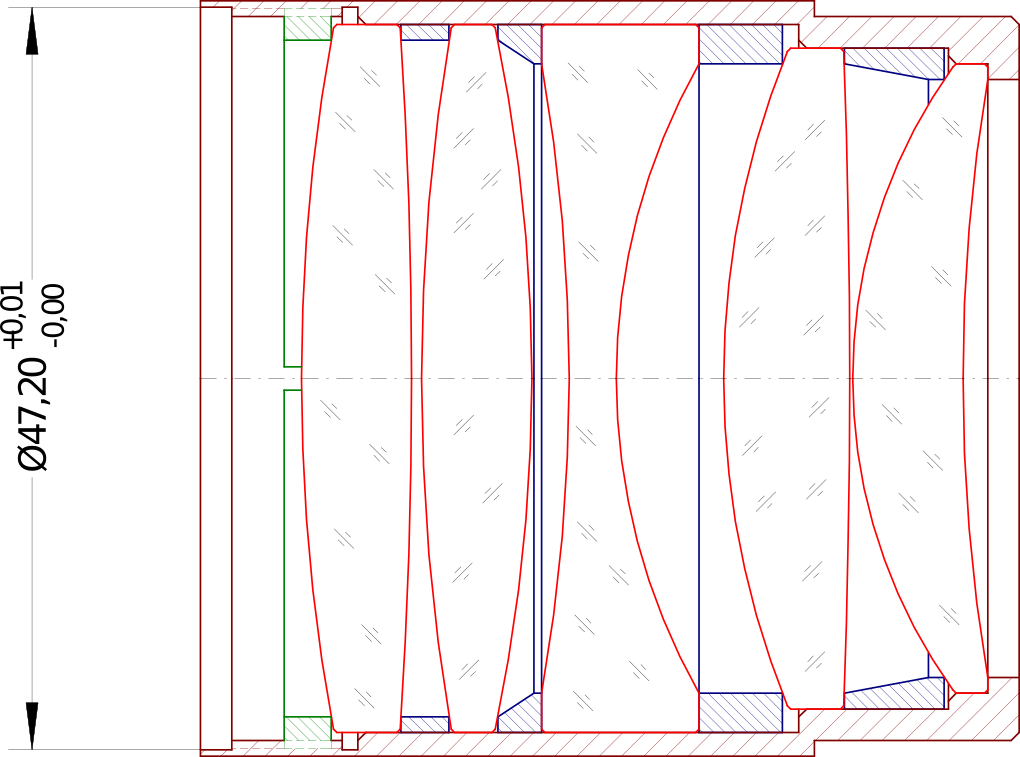
\includegraphics[width = \textwidth]{obj}
          \caption{Section of the custom objective, red parts are the lenses, while the rest is the housing.}
         \label{objsection}
     \end{subfigure}
     \hfill
     \begin{subfigure}[b]{0.55\textwidth}
         \centering
         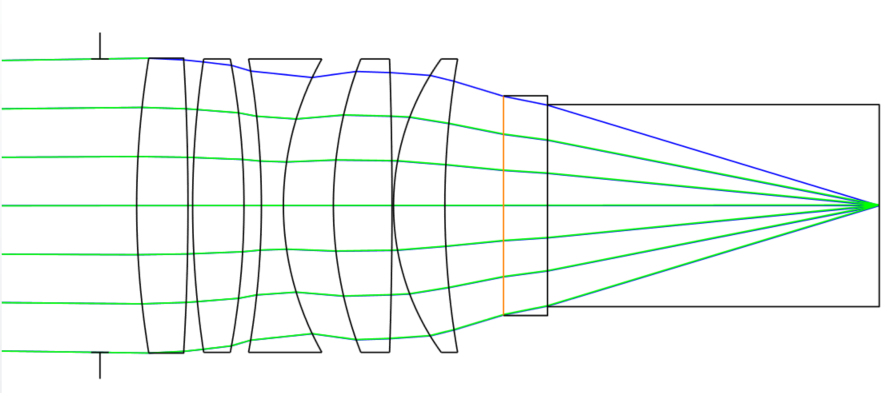
\includegraphics[width=\textwidth]{zeemaxobj}
         \vspace{1em}
         \caption{Zemax simulation of the objective. On the right, viewport and the vacuum chamber are also present.}
         %\label{fig:three sin x}

     \end{subfigure}
        \caption{}
      %  \label{fig:three graphs}
\end{figure}
The objective used to focus the light was already present in the system and had to be taken as it is. It is a custom objective by Sill optics placed outside vacuum, the section is in figure \ref{objsection}. It contains 5 lenses inside a mechanical housing, the aperture is about 47 mm large in diameter.
This objective has different purposes, it was designed keeping in mind: imaging of ions, addressing with red light and addressing of blue light. The objective has to perform all three of this jobs fairly well, which means it has light transmission >90 \%, every lenses is AR coated, numerical aperture of NA = 0.3. Moreover, it is telecentric, which means that the focus spot should move perpendicularly to the optical axis if the beam is steered.
 Lastly it was also designed to take into consideration the fact that it is placed out of vacuum, the light after the objective has to go through a 6 mm fused silica viewport before entering the vacuum and after further 40 mm encounters the ions. The focal length of the objective is 54.07 mm at 729nm. The objective is also mounted on a 3 dimensional translational stage to allow for imaging and addressing calibration.\\
The AOD is from Gooch \& Housego, model 4120-3. It has a specified central frequency of 120 MHz, with 50 MHz, bandwidth, so the driving frequency ranges from 95 to 145 MHz with a maximum RF power of 0.3 W. Therefore, the angle of deflection should be $\pm 0.86^{\circ}$ (:|).  In this bandwidth the diffraction efficiency should remain above 75 \% and have an average of 83 \%. Further light is lost as much as 3\% of due to insertion losses. The active aperture measures $3\times 3$ mm, and the polarization has to be horizontal when entering the AOD, while it gets rotated during diffraction, as the specified output polarization is vertical.

\section{Design simulation}
The setup in figure \ref{addressingsetup} has been simulated with the software Zemax. The simulation had the purpose of assessing the performance of the setup, i.e. checking the viability of the setup and see if it meets all requirements. It was also used to find the best lenses for building the setup and the best placement. Not everything was simulated, bu only the essential parts. This includes the four lenses, the objective, the viewport and the vacuum chamber. As there is no option to simulate an AOD, it was not taken in consideration, instead the simulation started at the output of the AOD as described below. Mirrors and beam splitters also do not alter drastically the optical path and therefore there was no need to simulate them.
\begin{figure}[H]
\centering
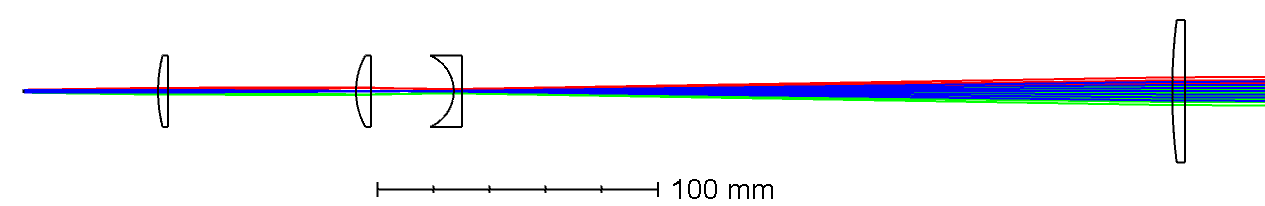
\includegraphics[width = \textwidth]{zemax3d}
\caption{Zemax simulation of the setup. Rays propagate from left to right, only the four lenses are displayed, objective and image plane are far on the right. Different colors indicate different fields at different angle}
\label{zemaxview}
\end{figure}
The simulations start by specifying the input fields, these represent the physical light beam. To account for the different angled beams at the output of the AOD, three different fields has been simulated. One is along the optical axis, while the other two are angled corresponding to the extrema of the AOD bandwidth, so $\pm0.86^{\circ}$. Therefore the propagation of these beams represents three different situations of beam direction and should also give an idea of the behaviour in between the extrema. Next, the four lenses of the setup were inserted in Zemax, initially with variable radius and thickness. The Zemax file of the objective came from the company which designed it and was simply imported in the project. After the objective the 6mm viewport glass was included and then vaccum for 38.6 mm, which is the distance between the outer facet of the glass and the ion axis. The image plane was therefore set here. The distance between the last lens of the objective and the viewport was unknown, but a good estimation\footnote{A posteriori, this assumption was not well suited and lead to some errors in the test setup. The correct value could be found by simulating the imaging setup and optimizing this distance to get the focus onto the camera.} allowed to progress with the simulation.
They physical simulation in the software was carried out with the tool Physical Optics Propagation (POP). POP works by propagating a wavefront represented by an array of discrete points. The array is propagated through every optical component and free space. This method can be used to simulate coherent Gaussian beam with high precision as well as wave phenomena such as diffraction and aberrations. The initial value given to the propagator was the waist of the collimated beam out of the AOD. Since the beam going to the AOD comes from a fiber collimator, the value specified was taken from the datasheet of the fiber collimator, namely Sc\"after + Kirchhoff 60FC-M8-33 \cite{fibercollimator}. Therefore, the specified waist was 0.72 mm.
\begin{figure}
     \centering
     \centering
     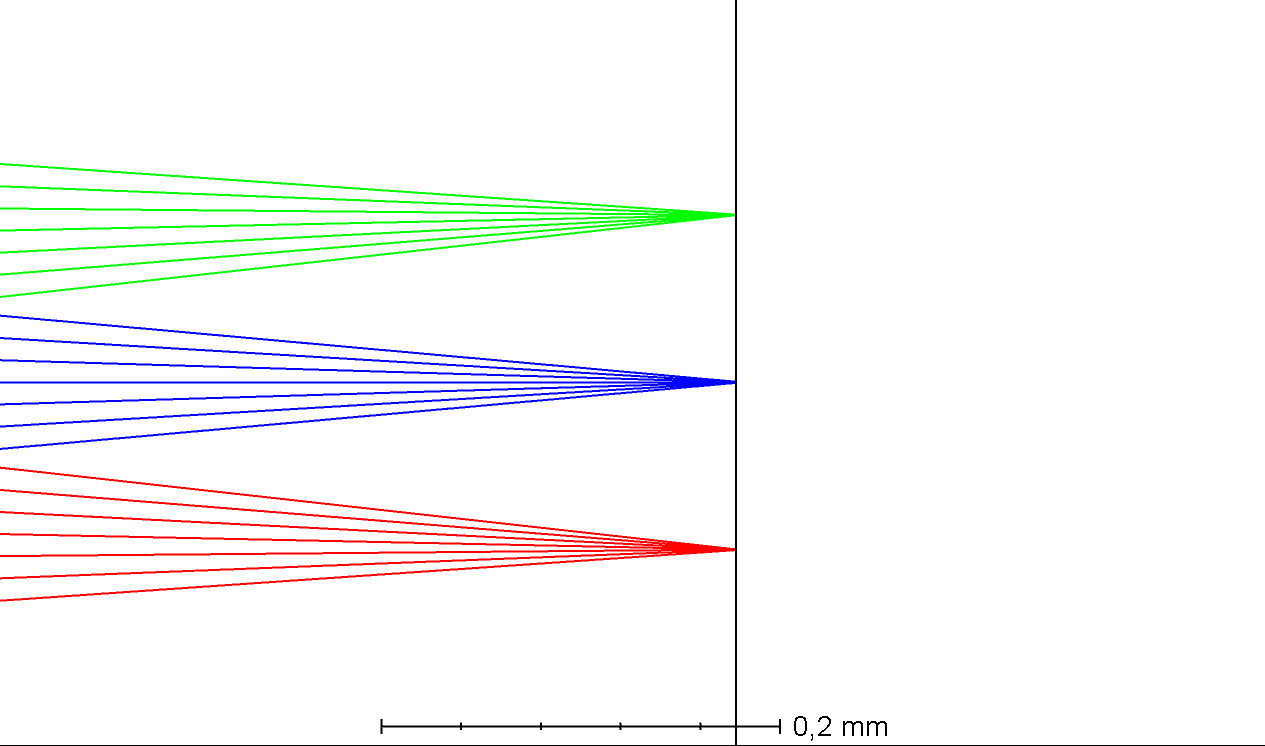
\includegraphics[width=.8\textwidth]{img/zemaxrange}
     \caption{Zemax simulation at the image plane, where the ions are. The three colors are three different fields with different angles that are focues at different position along the ion string. The full addressing range here displayed is about 168 $\mu$m.}
     \label{zemaxrange}
\end{figure}

\begin{figure}
    \centering
    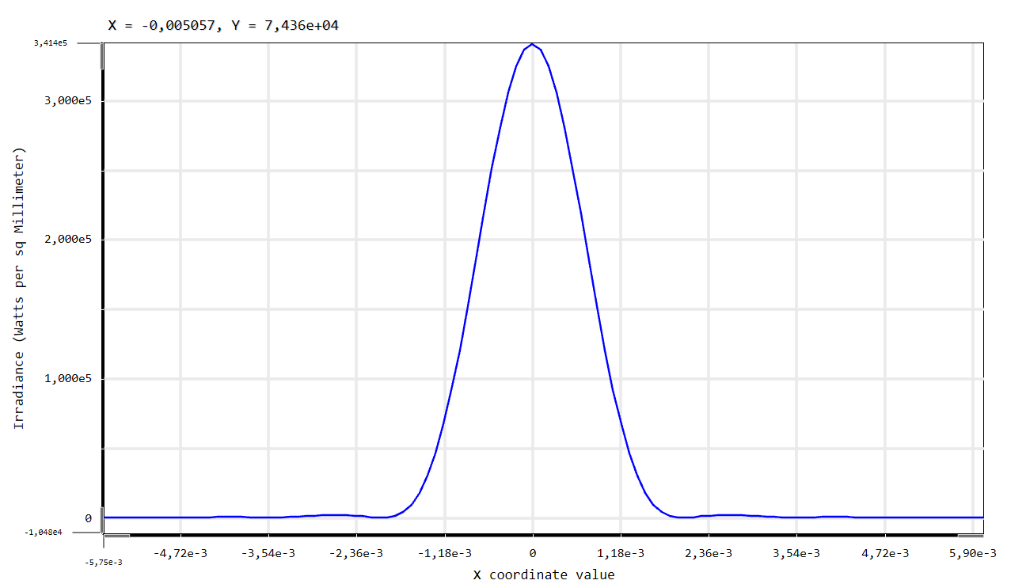
\includegraphics[width=.8\textwidth]{img/zemaxfocus}
\caption{POP of the central field at the ion position, $x$ cross section is displayed.}
\label{zemaxfocus}
\end{figure}
The first step of the simulation work was to find the appropriate lens to build the setup. The thickness and the radius of the lenses was optimized trying to achieve the best focus spot while maintaining a good addressing range. Once obtained the desired situation, the lenses were found with the Zemax tool \emph{Stock Lens Matching}. Basically the tool compares the simulated lenses with those in a catalogue from different companies and find the closest match. We opted to rely on the provider Thorlabs, so the search was limited to this company. Found lenses were in order from left to right LA-1059, LA-1131, LA-4252, and LA-1725 and can be seen in figure \ref{zemaxview}. Once the desired lenses were found, their Zemax files provided by the company were imported in the project and further optimization was carried on.\\
The second step was to optimize the lenses position always in view of finding the best focus spot while keeping a good addressing range. This was done using the optimiing tools of Zemax and the merit function. The software can perform multivariate analysis and minimize the focus spot depending on all the assigned variables, which in this case were the distance between the lenses. The final results can be seen in figure (), the addressing range is 168 $\mu$m, while the waist is $1.3\,\mu$m.\\
 Another important parameter for the performance of the setup is the addressing error. In the case of the beam focused on one ion, the addressing error is the leaking light on the neighbours ions. It can be a problem in the case of aberrations that produce bumps on the side of the main Gaussian peak. Especially in the case of diffraction limited system, the profile of the beam is a sinc function that can have more local maxima around the central peak. To estimate the addressing error, two ions are placed next to each other at 5.6 $\mu$m, and the respective addressing beam has been simulated. The intensity profile has been plotted in figure \ref{zemaxaddrerror.png} and addressing error is calculated as $I_1(x_2)/I_1(x_1)$, where $I_1$ is the intensity profile of the beam focused on the left ion and $x_1,x_2$ are the positions of the two ions. From the simulations we get $I_1(x_2)/I_1(x_1) \simeq 9 \times 10^{-4}$.\\
 \begin{figure}
 \centering
 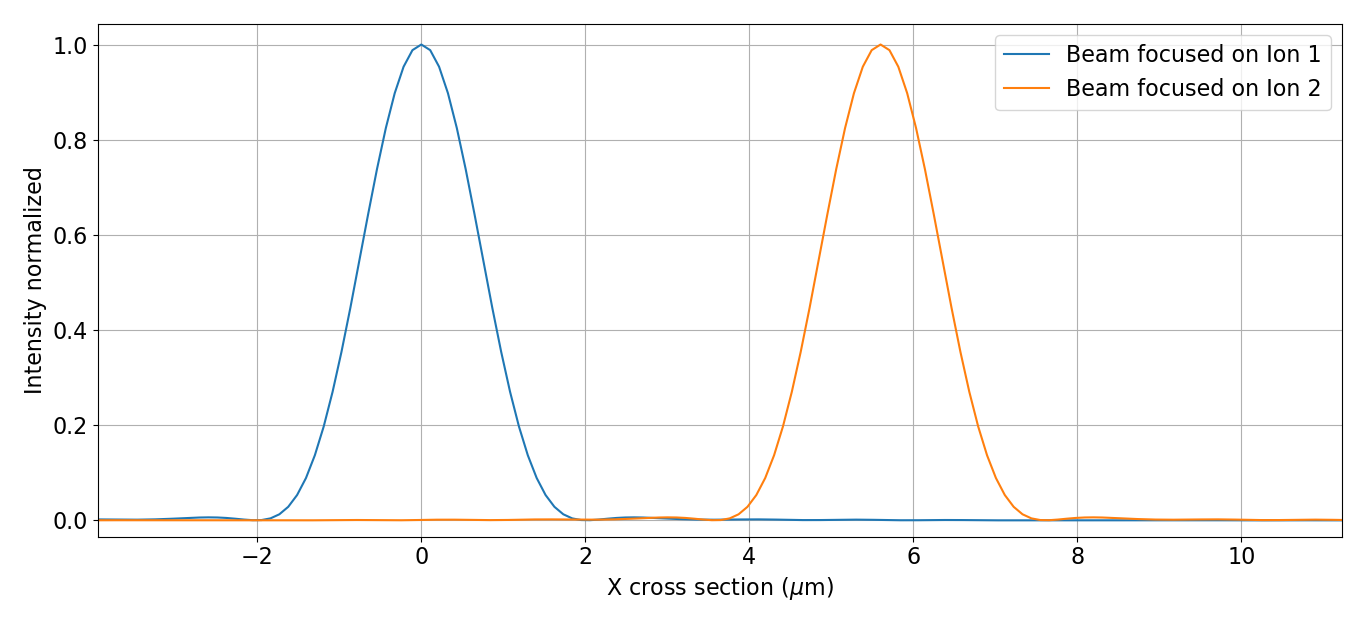
\includegraphics[width = .9\textwidth]{zemaxaddrerror.png}
 \caption{Beam focused at two different positions, where ions have their equilibrium position. From estimation of the addressing error can be made.}
 \label{zemaxaddrerror.png}
 \end{figure}
Another aspect that was simulated is the beam profile inside the trap. Optical access to the trap is limited and a tightly focus beam also has a large divergence, which could lead to clipping on the trap's blades or compensation electrodes scattering light all around the trap and thus creating problems. In figure \ref{clippingtop} the top view of the trap is plotted. The blue line represents the radius $W(z)$ from equation \ref{waistprofile} of the addressing beam in the case of a waist $W_0$ of 1 $\mu$m. There is no apparent clipping, and the main problem seems to be the compensations electrodes. Since the the beam is Gaussian, there is always a clipping part. To determine the fraction of power lost due to clipping on the compensation electrodes, we can calculated the transmitted power through the electrodes:
\begin{equation}
P_{t} = \int_{-\infty}^{\infty}\text{d}y \int_{-x_c/2}^{x_c/2}\text{d}x P(z),
\end{equation}
where $P(z)$ is the power of the Gaussian beam, and $x_c$ is the horizontal position of the compensation electrode. The integral can be computed numerically at position $z$ of the electrodes. The result is plotted in figure \ref{lossesplot}, where the lost power $1-P_{t}$ is plotted as a function of the waist $W_0$.
\begin{figure}
      \centering
        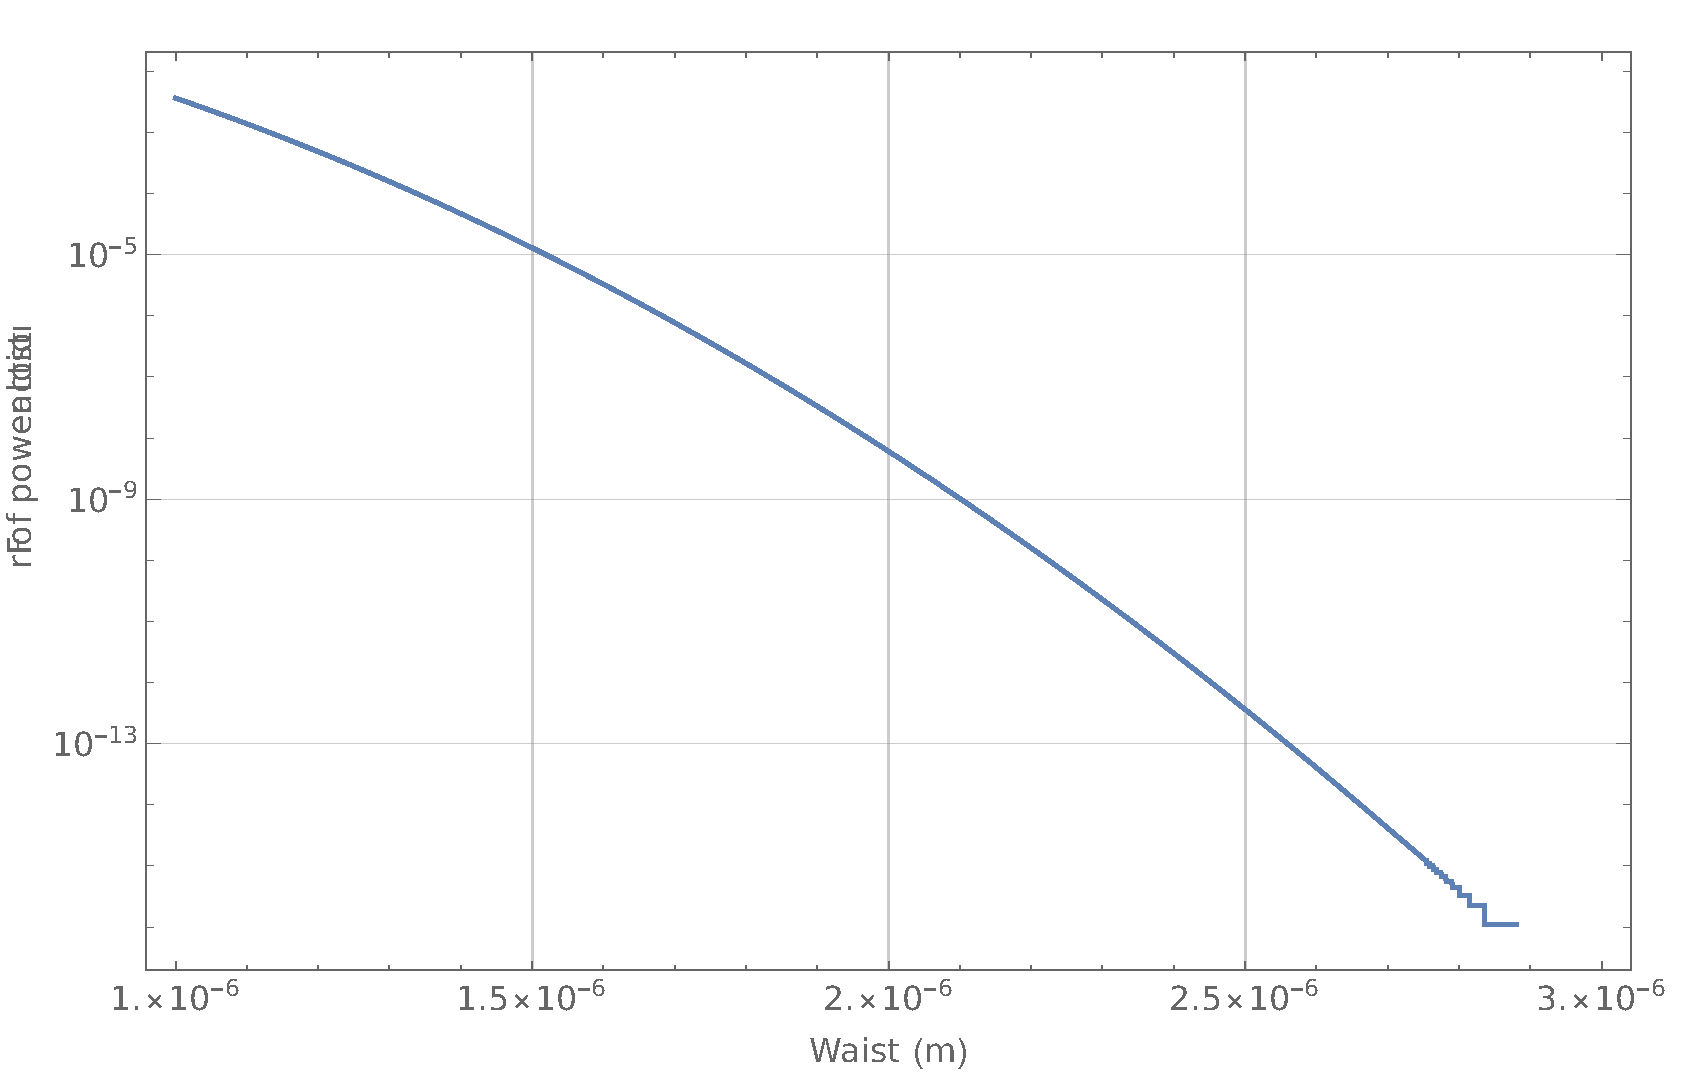
\includegraphics[width=.8\textwidth]{img/clipping2}
        \caption{Losses on the compensation electrodes as a function of the beam waist}
        \label{lossesplot}

\end{figure}

\begin{figure}
     \centering

     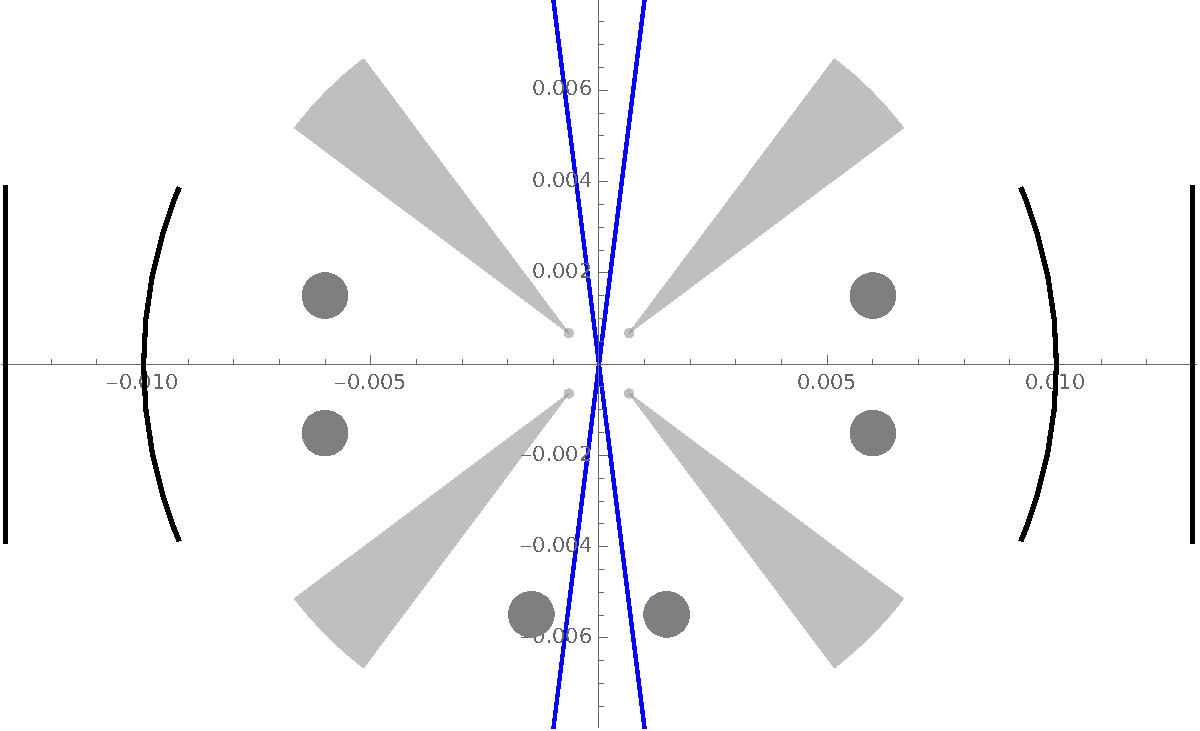
\includegraphics[width=.8\textwidth]{img/clipping}
     \caption{Top view of the trap and addressing beam. Grey circles are the compensation electrodes, blue is the radius $1/e^2$ of the beam, while the black arches representes the mirrors of the cavity.}
     \label{clippingtop}
     \end{figure}



\section{Physical implementation}
Once the simulations gave satisfactory results, a test setup was built. The idea of building first a test setup on a different optical table from the main experiment was to check if the system was working as intended, and asses its performance. Due to physical access problems, in the final system there is no space to place a beam profiler, or a polarimeter, and after the objective there is no access to the vacuum and the trap. While on another table everything could be checked and tested to make sure everything was working as expected. The results of the measurements obtained on this test setup are presented in the next chapter.\\
Afterwards, the real system was built. The building process was tricky, as the system is particularly sensitive to aberrations. Furthermore, there was not much room for alignment errors, since the trap and ion have to be hit perfectly. For this reason the alignment was essential. In order to make sure the addressing beam would hit the ion, a counter propagating red beam was send in the opposite direction, starting from the ion back to the objective and back to the addressing path. Since the lenses of the addressing are antireflecting coated for 393 nm, the reflection of the red beam was visible and it was possible to align every optical component. The photo of the final system is in figure \ref{photosetup}. Here the collimating lens is mounted on a 3D translation stage with Newport screws for fine tuning calibration of the focus position. Manual screw has been later replaced with remote controlled one always from Newport, model PZA12. An iris is also used to block the zeroth order beam from the AOD. Moreover, The AOD is placed on a rotational mount that allows to tilt it in two directions. One direction was used to find the Bragg angle to achieve maximum diffraction, and the other can be used to tilt the axis over which the AOD sweeps. This can be used to compensate for an ion string which is not exactly parallel to the AOD sweeping direction.

\begin{figure}[H]
\centering
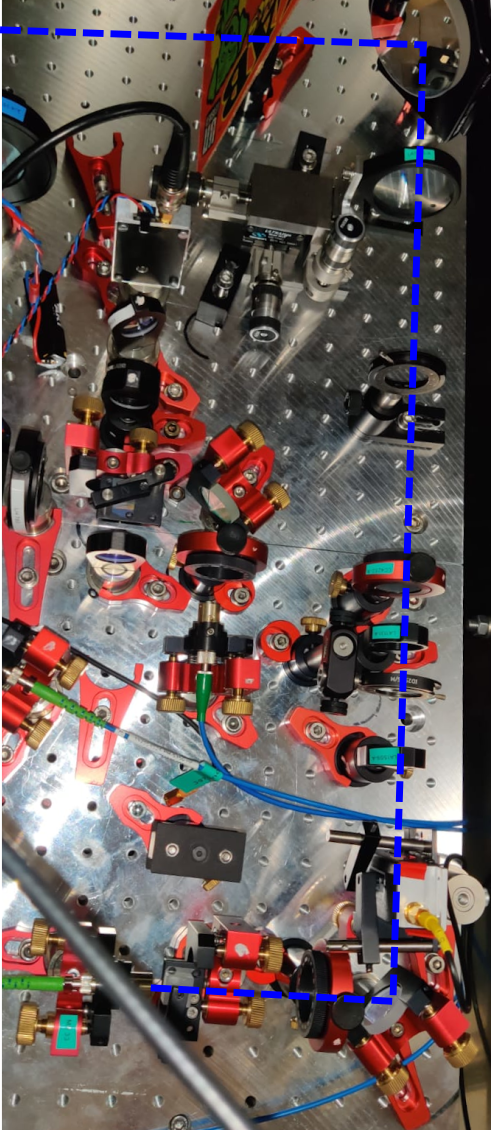
\includegraphics[scale = 1.3]{photosetupnice.png}
\caption{Photo of the final setup. The blue dashed line is the beam path starting from bottom left at the fiber collimator, all the way to the top where a mirror deflects the beam to send it to the beam splitter.}
\label{photosetup}
\end{figure}



%Measurement results
% !TEX root = main.tex

\chapter{Experimental results}
\label{ch:results}
This chapter collects the key experimental results obtained during my master's work:
\begin{itemize}
\item Section \ref{sec:resultaod} contains the characterization of the AOD.
\item In Section \ref{sec:fullsetup} the characterization of the test setup is presented. Polarization, stability, and focus spot have been checked. In particular, two methods have been used to measure a $\mu$m focus spot: razor blade scans, and small pixel size camera.
\item In Section \ref{sec:finalsetup} the results from experiments with trapped ions are presented. First, single-qubit manipulation via Ramsey interferometry, which also allowed for a check of addressing performance. Second, a cQED experiment where single photons were generated from a single ion in a string, via a cavity-mediated Raman process (Section \ref{sec:ramanprocess}).
\end{itemize}
\section{AOD}
\label{sec:resultaod}
The two main parameters we are interested in are the diffraction efficiency and the response time. For the diffraction efficiency we measured the total output power of the light $P_{tot}$ and then the power of the first diffracted order $P_{1}$. Diffraction efficiency is defined as the ratio between the two
\begin{equation}
\label{eq:de}
\text{DE} = \frac{P_1}{P_{tot}}.
\end{equation}
The response time is the time it takes for the light to move to a new position corresponding to a RF frequency change. The measurement of the response time gives us an idea of how long it takes to switch from one ion to the other.\\
Before measuring the diffraction, the optimal RF power to drive the AOD has been found by maximizing the power of the first diffracted order with the AOD set at its central frequency. Power measurements of the light were done with a Thorlabs PM100D, and the AOD was driven with an amplifier and an RF signal generator. The highest efficiency at the central frequency was found for an RF power of 0.11 W, and for the rest of the measurements it was kept at that value. Furthermore, to optimize the linear input polarization, a PBS followed by a half-waveplate were placed before the AOD, the waveplate was rotated to maximize the power of the diffracted light. In Figure \ref{DE} a plot of the measured diffraction efficiency as a function of the RF frequency is displayed. Within a bandwidth of 50 MHz from 105 MHz to 155 MHz, we can see that more than 70 \% of the light is in the first diffracted order as expected from the datasheet (Appendix \ref{sec:aoddata}), even though the bandwidth looks shifted with respected to the nominal central frequency of 120 MHz.\\
In order to measure the response time, a voltage controlled oscillator (VCO) was used to generate the RF signal. The VCO was supplied a square wave that alternated between two voltages corresponding to two different frequencies $\sim 96$ and $\sim 127$ MHz. The laser light diffracted into the -1 order was measured with a photodiode. The photodiode was aligned with the light at one particular frequency, such that when the light moves, the beam would not hit the diode and the signal generated changes. In Figure \ref{response}, the signal of the photodiode, together with the supplied VCO signal are plotted. Response time is $\sim 8\,\mu$s, with $3\,\mu$s delay and $5\,\mu$s rise time. From the beam diameter (2.14 mm, $1/e^2$ of intensity) and the acoustic velocity in the crystal (0.65 mm/$\mu$s, Appendix \ref{sec:aoddata}) we expect $4.9$ $\mu$s rise time, while the delay indicates that the distance between the piezo and the edge of the beam is 1.95 mm.

\begin{figure}
\centering
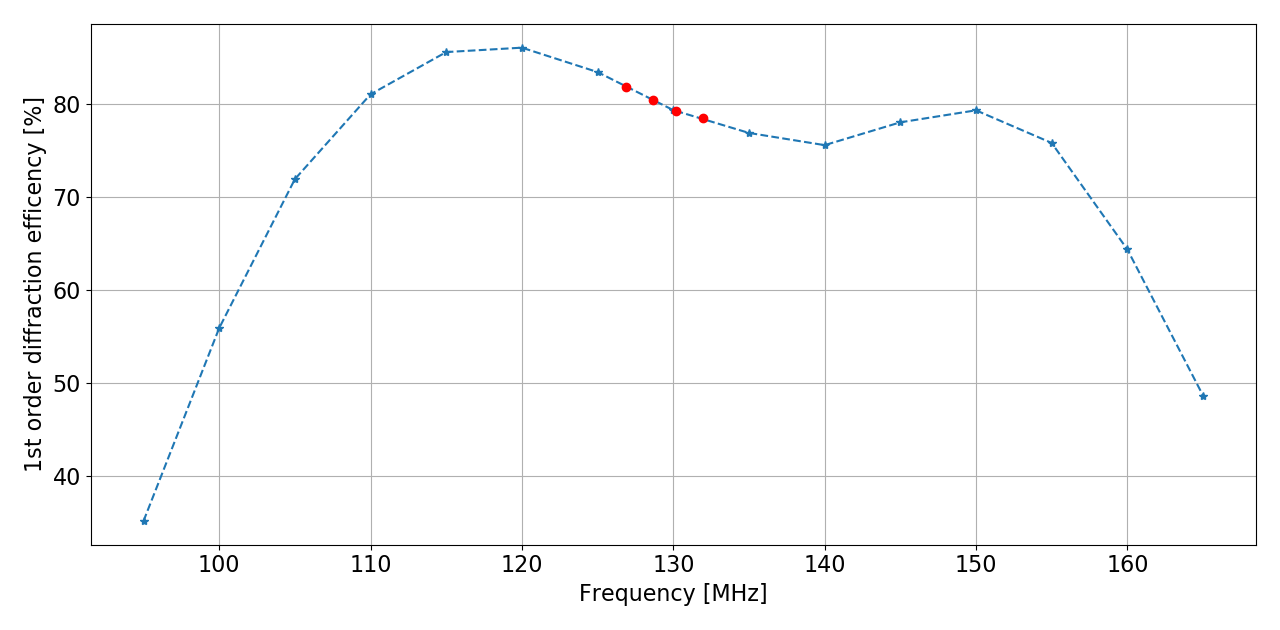
\includegraphics[width = .95\textwidth]{DE2}
\caption{Measurement of the diffraction efficiency of the AOD as a function of the RF driving frequency (Equation \eqref{eq:de}). Blu stars indicate the measured points. Red points indicate the expected frequencies associated with addressing 4 ions for an axial COM frequency of 780 kHz (the conditions for the experiment presented in Section \ref{sec:singlequbitmanipulation}), the theoretical separations are 5.15 $\mu$m for the two outer ions, and 4.77 $\mu$m for the inner ions.}
\label{DE}
\end{figure}

\begin{figure}
\centering
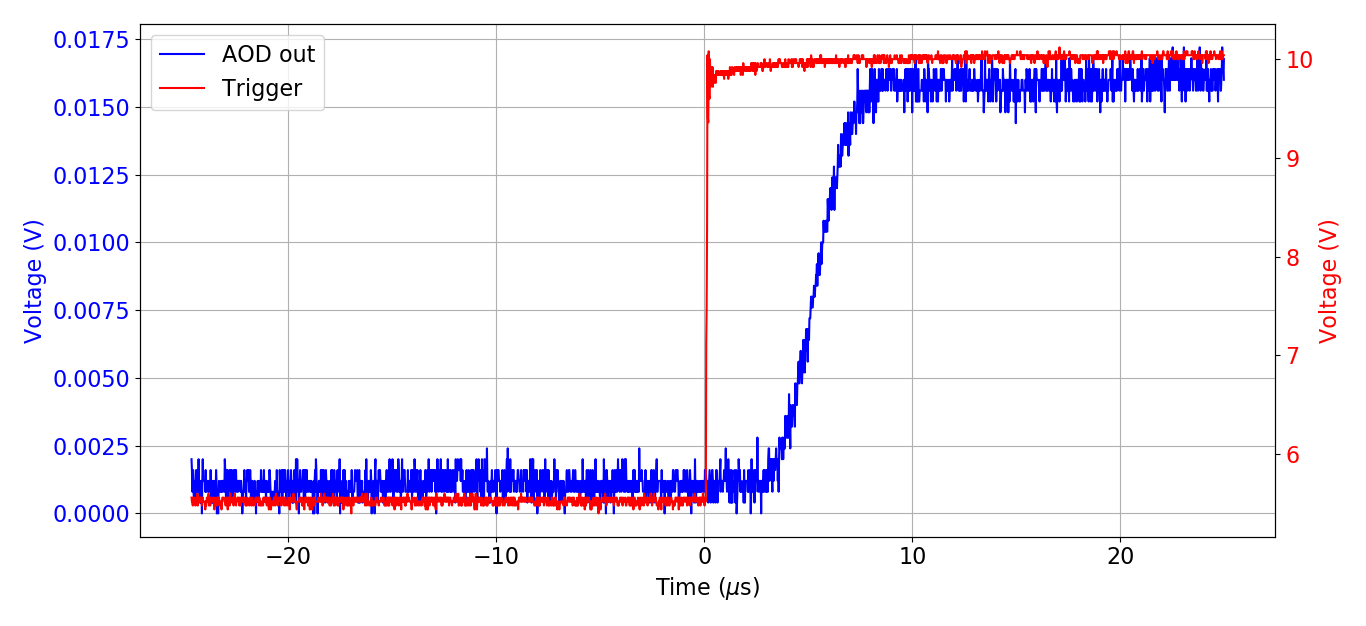
\includegraphics[width = .95\textwidth]{response}
\caption{Response time of the AOD, plotted are the photodiode signal in blue on the left $y$ axis, and the VCO voltage is in red on the right axis. The voltage of the VCO determines the frequency of the RF sent to the AOD. The change here corresponds to a frequency shift of $\sim$31 MHz between $\sim 96$ and $\sim 127$ MHz. At the highest voltage, the photodiode measures the -1st diffracted light.}
\label{response}
\end{figure}

\section{Full test setup characterization}
\label{sec:fullsetup}
The test setup was built on an optical table with a spare objective since the one installed in the vacuum chamber was already in use for ion imaging. The layout of the system in Figure \ref{addressingsetup} was replicated.

\subsection{Waist: Knife-Edge method}
\label{sec:knifeedge}
\begin{figure}[H]
\centering
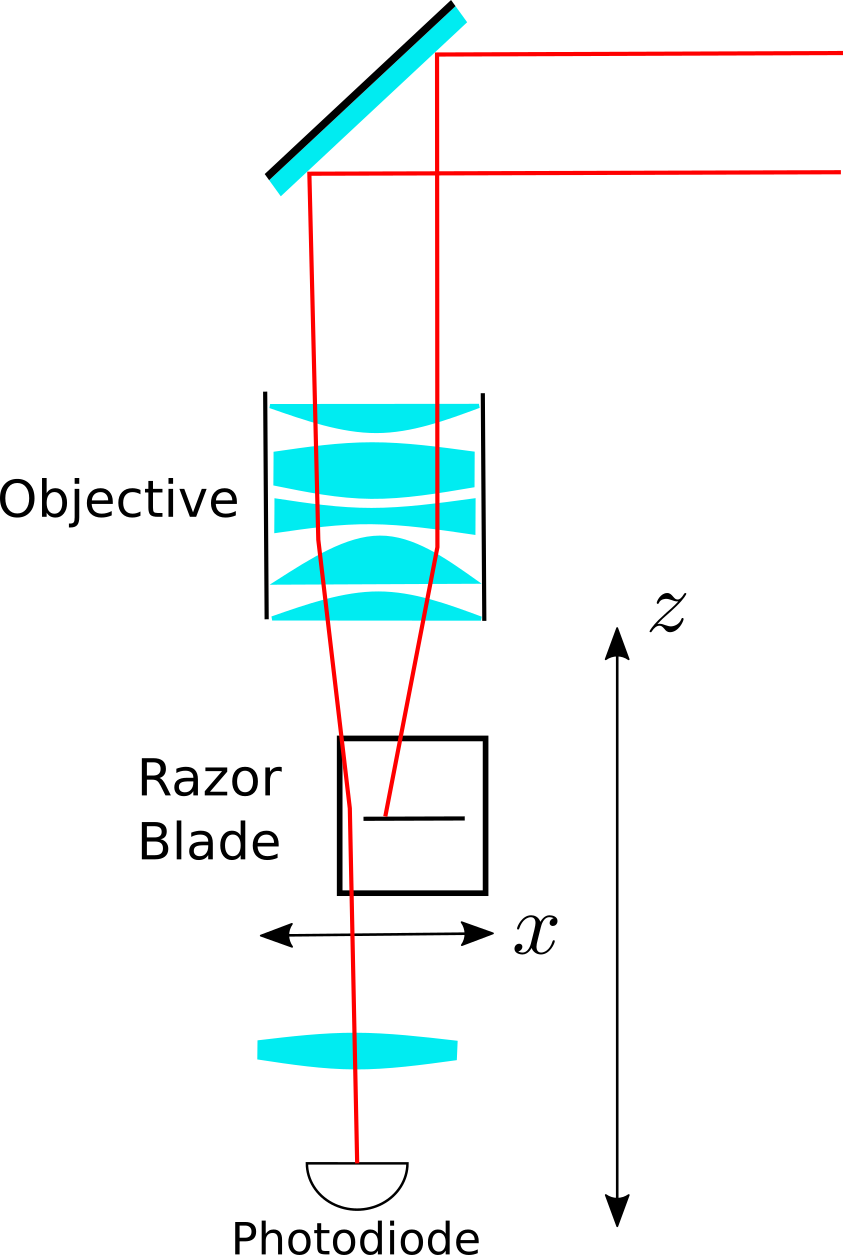
\includegraphics[scale = 1.1]{razorsetup}
\caption{Scheme of the razor scan. A translation stage allows for moving the blade in the direction x, perpendicular to the beam, and z, along the beam.}
\label{razorscan}
\end{figure}
Measuring a micrometer scale waist is not an easy task, the first method applied consisted of mounting a razor blade on a translational stage. The setup used is showed in Figure \ref{razorscan}, after the objective the blade is present, and since the beam is quickly diverging after the focus, a lens is used to refocus the light into a photodiode. The stage is moved in the $x$ direction cutting the beam perpendicularly such that the blade is scanning the beam profile. A filter was inserted in order to not saturate the photodiode.
In the $z$ direction the stage was controlled with a manual screw with resolution of $1\,\mu$m. While in the $x$ direction, the stage had to be moved with sub-micrometer precision, so instead there was a piezo actuator controlled by custom software. The same software also controlled a multimeter that measured the voltage of the photodiode. To get the profile $W(z)$ (equation \eqref{waistprofile}) of the beam, the measurement procedure was as follows
\begin{itemize}
\item Position blade at desired $z$ coordinate
\item Scan beam in $x$ direction with blade
\item Shift $z$ direction
\end{itemize}
The procedure is repeated for sufficient values of $z$ to scan at least a few Raylegh ranges. The beam width can be calculated from the scans by fitting the data with equation (2) of \cite{knifeedge}. In Figure \ref{examplerazorscan} we report an example of a scan that gave a minimal waist. The errorbars come from statistical average, every data point is a mean over 5 measurements, and the error is the standard deviation. The fit in this case gave a width $W$ (beam width $1/e^2$) of $3.47\pm 0.06\,\mu$m, the smallest width obtained with this method, but significantly broader than the 1 $\mu$m simulated waist. Furthermore, the profile $W(z)$ was not symmetric and could not be fitted with equation \eqref{waistprofile}. A possible explanation is that with this typically commercially-available razor blade, the accuracy is limited by the positioner and the blade roughness. The latter was not known at the few micrometer scale of the beam waist. In comparison, authors of \cite{Cannon:86} have used, instead of a common razor blade, a glass substrate etched with an effective knife-edge features with which they were able to measure a 1 $\mu$m waist.
\begin{figure}
\centering
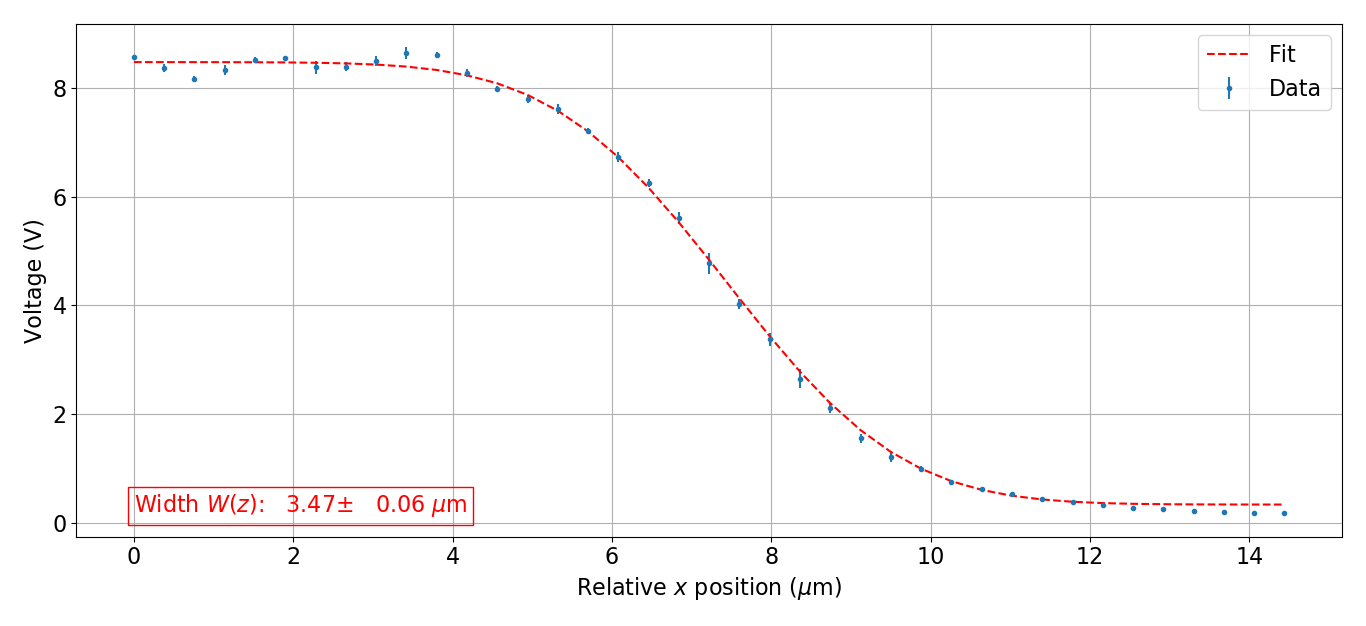
\includegraphics[width=1\textwidth]{img/razorscan}
\caption{Razor scan at the waist of the beam $z=0$}
\label{examplerazorscan}
\end{figure}


\subsection{Waist: Camera}
\label{waistcamera}
Since the Knife-Edge method did not prove that we had achieved our desired waist, a  more direct approach has been subsequently adopted. We measured directly the beam with a camera from IDS model UI-1490LE-M-GL. This camera has a pixel size of 1.67 $\mu$m with no spacing between pixels. It should therefore be suitable to measure a focus spot with a $\mu$m precision. A 1 $\mu$m focus should hit one single pixel, and if aligned between two pixels, a Gaussian profile could also be fitted.
In addition, unlike the Knife-Edge technique, a camera provides 2-dimensional information about the beam shape and can be exploited to look for aberrations in the system. The setup is almost the same as Figure \ref{razorscan}, but the camera now replaces the razor blade, and there is no need for scanning in the $x$ direction, as the $z$ is enough to reconstruct the profile $W(z)$. An additional filter was used to optimize the light reaching the camera in order to not saturate it.
% \begin{figure}
%      \centering
%      \begin{subfigure}[b]{0.67\textwidth}
%          \centering
%          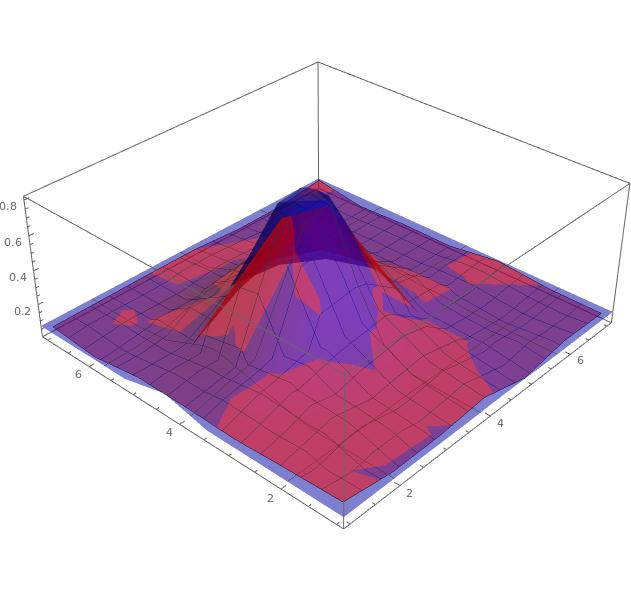
\includegraphics[width = \textwidth]{camera}
%           \caption{Fitted data from the camera. In red color, the normalized pixel value is displayed, while the blue curve is a fitted 2D Gaussian. On the axis there is the pixel number}
%      \end{subfigure}
%      \hfill
%      \begin{subfigure}[b]{0.3\textwidth}
%          \centering
%          
\includegraphics[width=\textwidth]{cameraoriginal}
%         \vspace{5em}
%          \caption{Original photo from the camera.}
%          %\label{fig:three sin x}
%
%      \end{subfigure}
%         \caption{}
%        \label{fig:camera}
% \end{figure}
For every desired $z$ displacement, a photo with the camera is taken, post processed, and then the camera is displaced to the new $z$ coordinate. Post processing is done by fitting the pixel values with a 2-dimensional Gaussian
\begin{equation}
P = A \exp\left\{-\frac{(x-x_0)^2}{2\sigma_x^2}\right\} \exp\left\{-\frac{(y-y_0)^2}{2\sigma_y^2} \right\}.
\end{equation}
The fit parameters are $A,x_0,y_0,\sigma_x,$ and $\sigma_y$. From the standard deviations $\sigma_x$ and $\sigma_y$ the beam width in the $x$ and $y$ direction at position $z$: $W_x(z),W_y(z)$ can be determined as $W_x(z) = 2\cdot 1.67\cdot \sigma_x$ and respectively $W_y(z) = 2\cdot 1.67\cdot \sigma_y$, where $1.67\,\mu$m is the pixel size (see caption of Figure \ref{gauss}). The full profiles $W_x(z)$ and $W_{y}(z)$ can be found in Figure \ref{cameraprofile}. Here anomalies can be noticed. The profile is asymmetric and does not follow equation \ref{waistprofile}, nonetheless a width $<2.5\,\mu$m has been measured. We decided to install the system and measure more accurately the waist with a single ion.
\begin{figure}
\centering
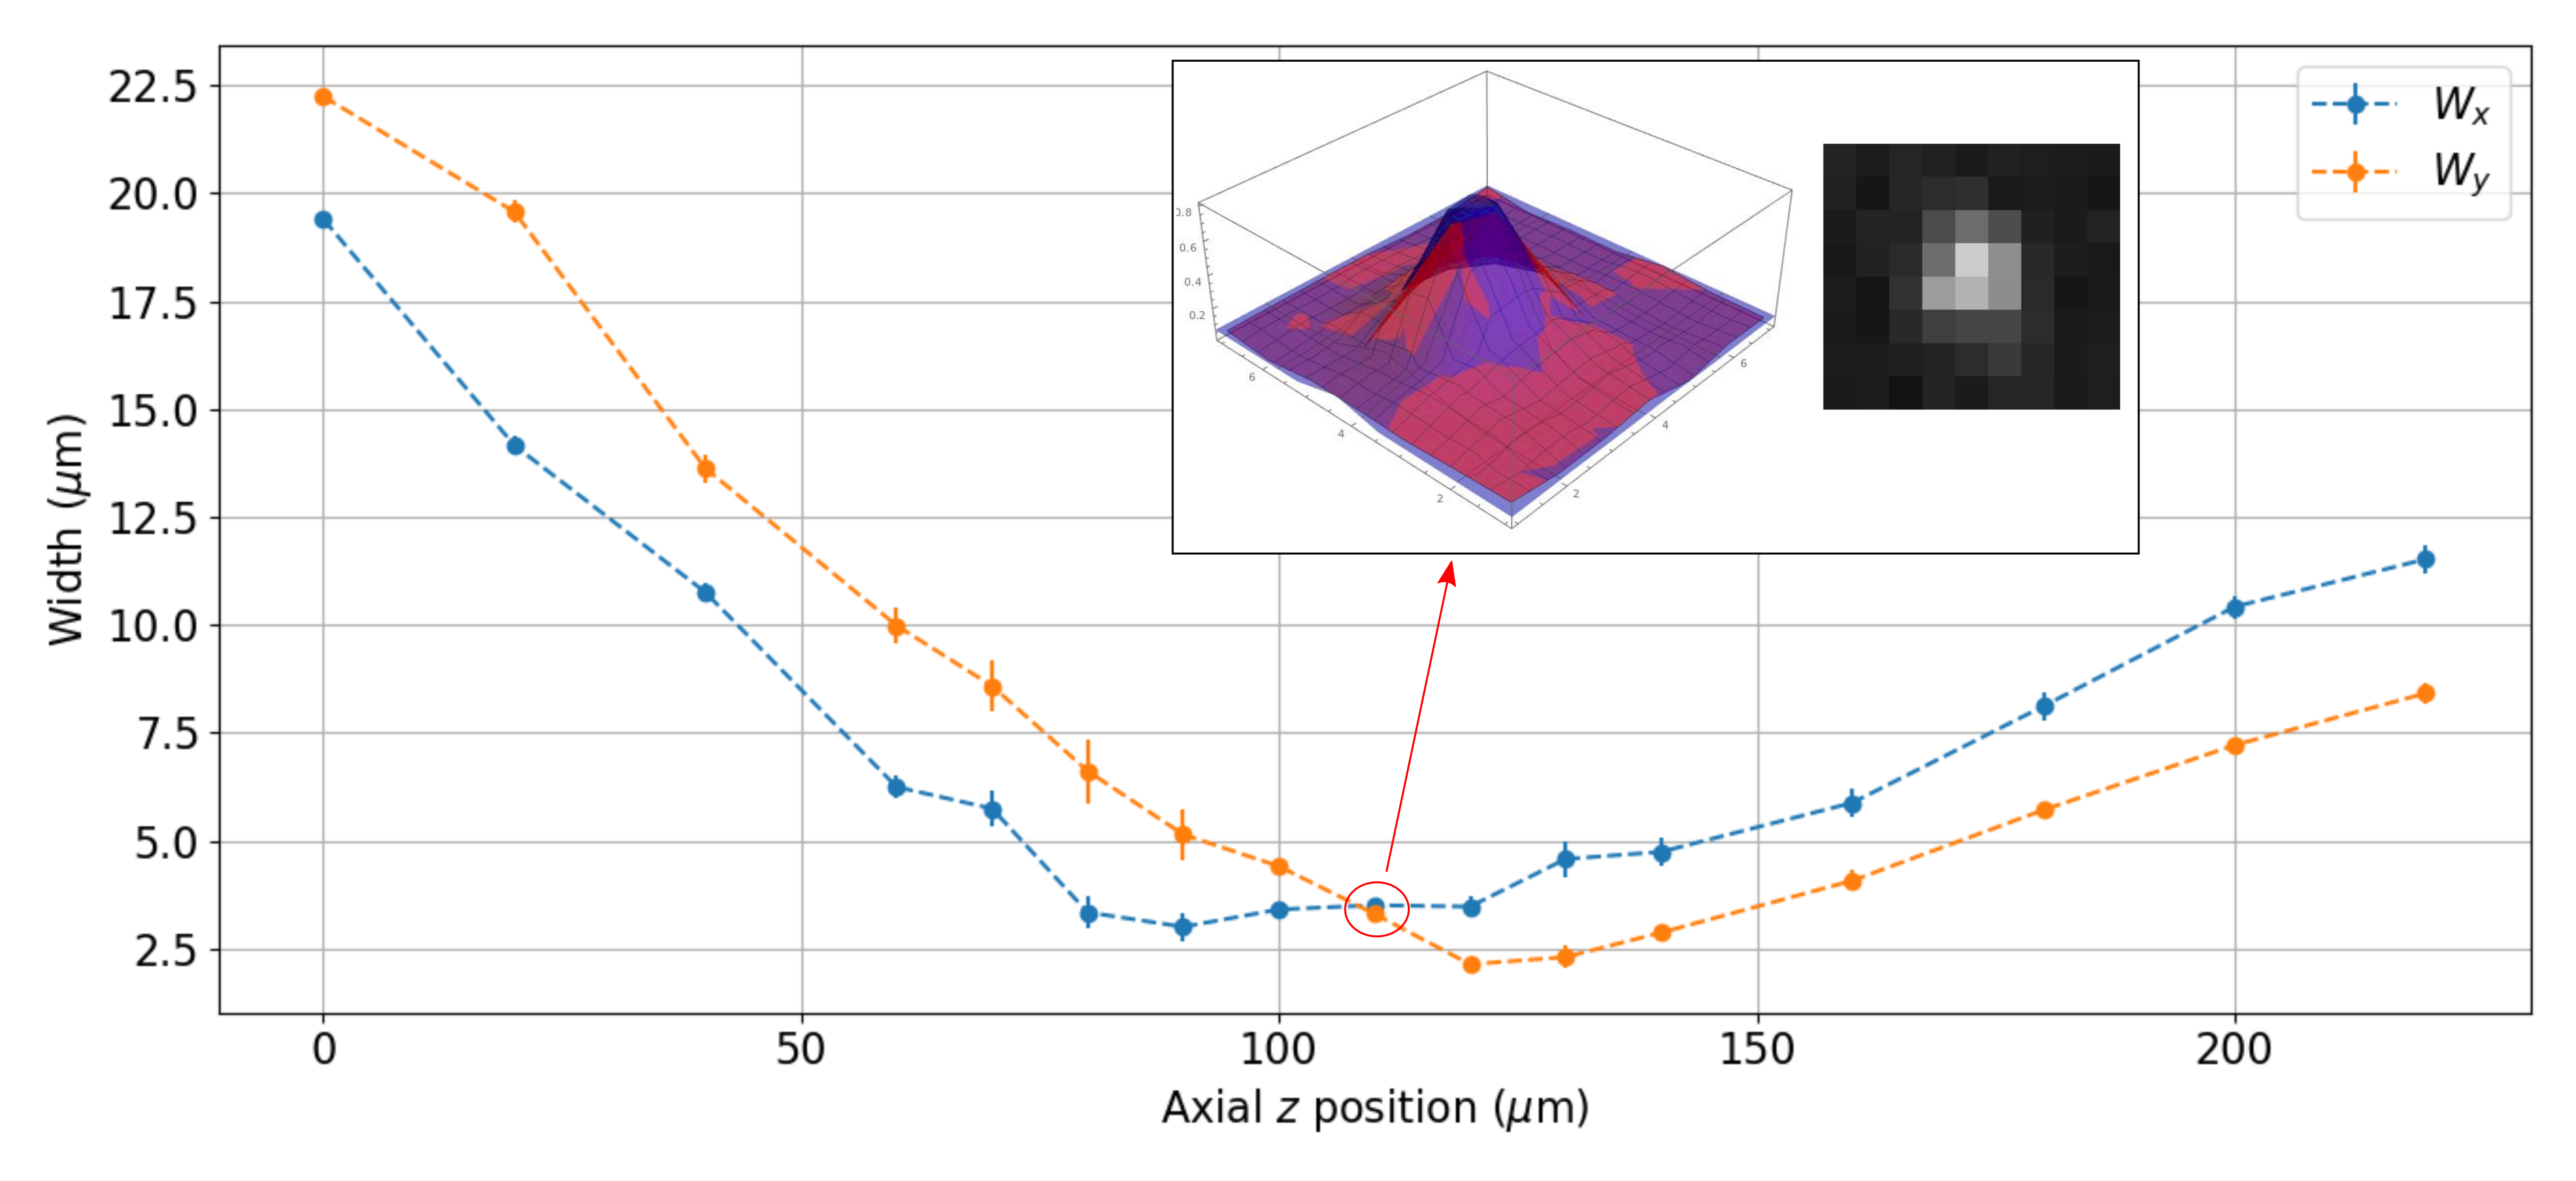
\includegraphics[width=1\textwidth]{cameraprofile_inset}
\caption{Profile of the Gaussian beam along $z$ measured with the IDS camera. Errorbars are estimated from fit. In the inset an example of raw data and Gaussian fit. In red color, the normalized pixel value is displayed, while the blue curve is a fitted 2D Gaussian. On the axis there is the pixel number.}
\label{cameraprofile}
\end{figure}

\subsection{Polarization}
\label{sec:polarization}
As discussed in the design Section \ref{sec:addressing} and in the Raman process \ref{sec:ramanprocess}, polarization is an important component as atomic transitions are polarization sensitive, thus the polarization capabilities of the system had to be tested. The goal is to allow for the generation of vertical, horizontal, left circular, and right circular polarization at the ion position and test how well they are achieved. Polarization can be changed with two plates: a half wave plate after the AOD, and a quarter wave plate right before the objective, see Figure \ref{addressingsetup}. In order to characterize the polarization at various points in the optical path of the addressing setup, the three Stokes parameters $S_i$ \cite{stokes} were measured with a polarimeter from Sc\"after + Kirchhoff series SK010PA.\\
Stokes parameters quantify the type of polarization of an electric field. Linear polarized light has Stokes parameters $S_2,S_3 = 0$, while $S_1 = \pm 1$ for horizontal and vertical polarization respectively. Circular polarized light has $S_1, S_2 = 0$ and $S_3=\pm 1$ for right hand and left hand circular polarization respectively.\\
The first step was to characterize the polarization after the waveplate after the AOD ($\lambda/2$, WP B, Figure \ref{addressingsetup}), the main result from this characterization is that horizontal polarization can be achieved immediately after WP B with an angle of $267.2\pm 0.1 ^{\circ}$, and vertical is achieved with an angle of $312.5\pm0.1^{\circ}$ obtained from fitting a sine on the first Stokes parameter. From the same fit, the semiperiod of the polarization is $45.3\pm 0.6^\circ$ consistent with the $45^\circ$ expected for a half waveplate.\\
Afterwards, we measured the polarization after the objective at the focus spot where the ions ideally sit. For this measurement we set the $\lambda/2$ WP B first at $267.2^\circ$, and then at $312.5\pm0.1^{\circ}$, for both numbers we measured the three Stokes parameters as a function of the $\lambda/4$ angle. Results are summarized in table \ref{polarizationstable}, in appendix \ref{app:polarization} the full plots are reported.
\begin{table}
\centering
\begin{tabular}{c c c c c c}
 \toprule
    {Desired polarization} & {$\lambda/2$ WP B ($^\circ$)} & {$\lambda/4$ ($^\circ$)} & Stokes 1 & Stokes 2 & Stokes 3\\ \midrule\midrule
   Horizontal & $267.2\pm 0.1$ & $49.7\pm0.1$ & 1.00 & -0.01 & 0.01\\
   Vertical   & $312.5\pm0.1$ & $48.1\pm0.1$ &  0.96 &  0.12 & -0.26 \\ \midrule
   Right circular & $267.2\pm 0.1$ & $4\pm 0.1$ &  0.05 & -0.02 & 1.00 \\
   Right circular & $312.5\pm0.1$ & $93.1\pm0.1$ & 0.10 & 0.01 & 1.00  \\\midrule
  Left circular & $267.2\pm 0.1$ & $95.4\pm0.1$ &  0.06 & 0.01 & -1.00  \\
    Left circular & $312.5\pm0.1$  & $3.1\pm0.1$ &  -0.20 & 0.06 & -0.98  \\ \bottomrule
\end{tabular}
\caption{Desired polarization at the ion position and angles of the waveplates $\lambda/2$ WP B and $\lambda/4$ (Ref. Figure \ref{addressingsetup}) that set the polarization. Numbers are found as maxima or minima of a sine fit of the polarization data in appendix \ref{app:polarization}. Measured Stokes parameter of the achieved polarization are given.}
\label{polarizationstable}
\end{table}

\subsection{Stability}
\label{sec:stability}
It is imperative to know the stability of the system in terms of polarization and beam pointing. This means knowing over the course of seconds, hours or days if the setup needs to be re-optimized or calibrated. First we measured polarization, it was set to be right circular at the ion position: $\lambda/2$ set to $267^\circ$, and $\lambda/4$ set to $4^\circ$. We recorded the three Stokes parameters for a total of one hour, this data is plotted in Figure \ref{polstability}. It can be seen that the polarization is stable within short term fluctuations (due to device precision) over a period of one hour.\\
Beam pointing stability is the stability of the focus position, which could drift in any direction. To test it, we recorded the position of the focus for a period of one hour with the camera. The camera was positioned at the focus with the same setup discussed in Section \ref{waistcamera}, and then a video was recorded. The video was later analyzed by tracking the brightest pixel over time. In Figure \ref{beampointing} we can see the horizontal $x$ and vertical $y$ position of such pixel. In the horizontal direction, fluctuations of one single pixel can be noticed, which could be a result of the light hitting between two pixels. In the vertical direction the fluctuations are in the order of two pixels, this could indicate that the position might have shifted by one entire pixel over this period. This means that the focus position is stable with an upperbound of $1.6\,\mu$m/hour. We have to consider that this measurement was taken on a open table, a more precise beam pointing stability measurement is carried out with ions in the closed mu-metal shield, see Section \ref{sec:singlequbitmanipulation}.

\begin{figure}[H]
\centering
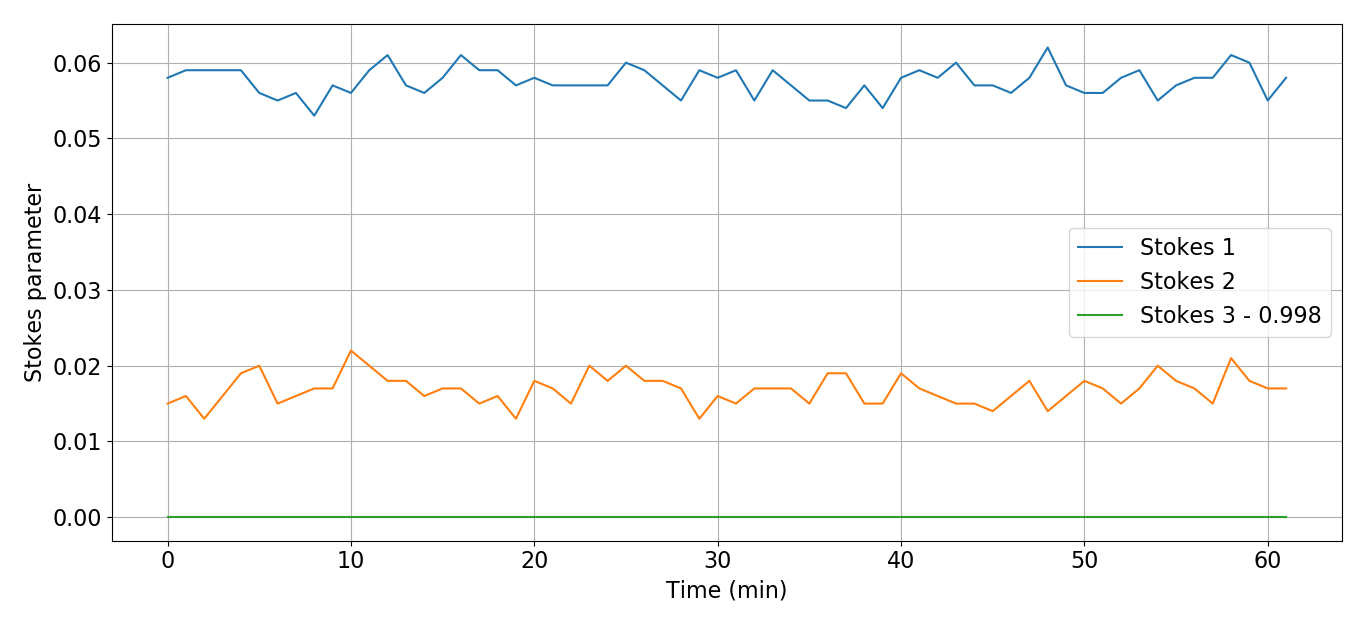
\includegraphics[width = .9\textwidth]{polstability}
\caption{Right circular polarization stability at the ion position over a period of one hour. To the third parameter $S_3$, 0.998 has been subtracted.}
\label{polstability}
\end{figure}

\begin{figure}[H]
\centering
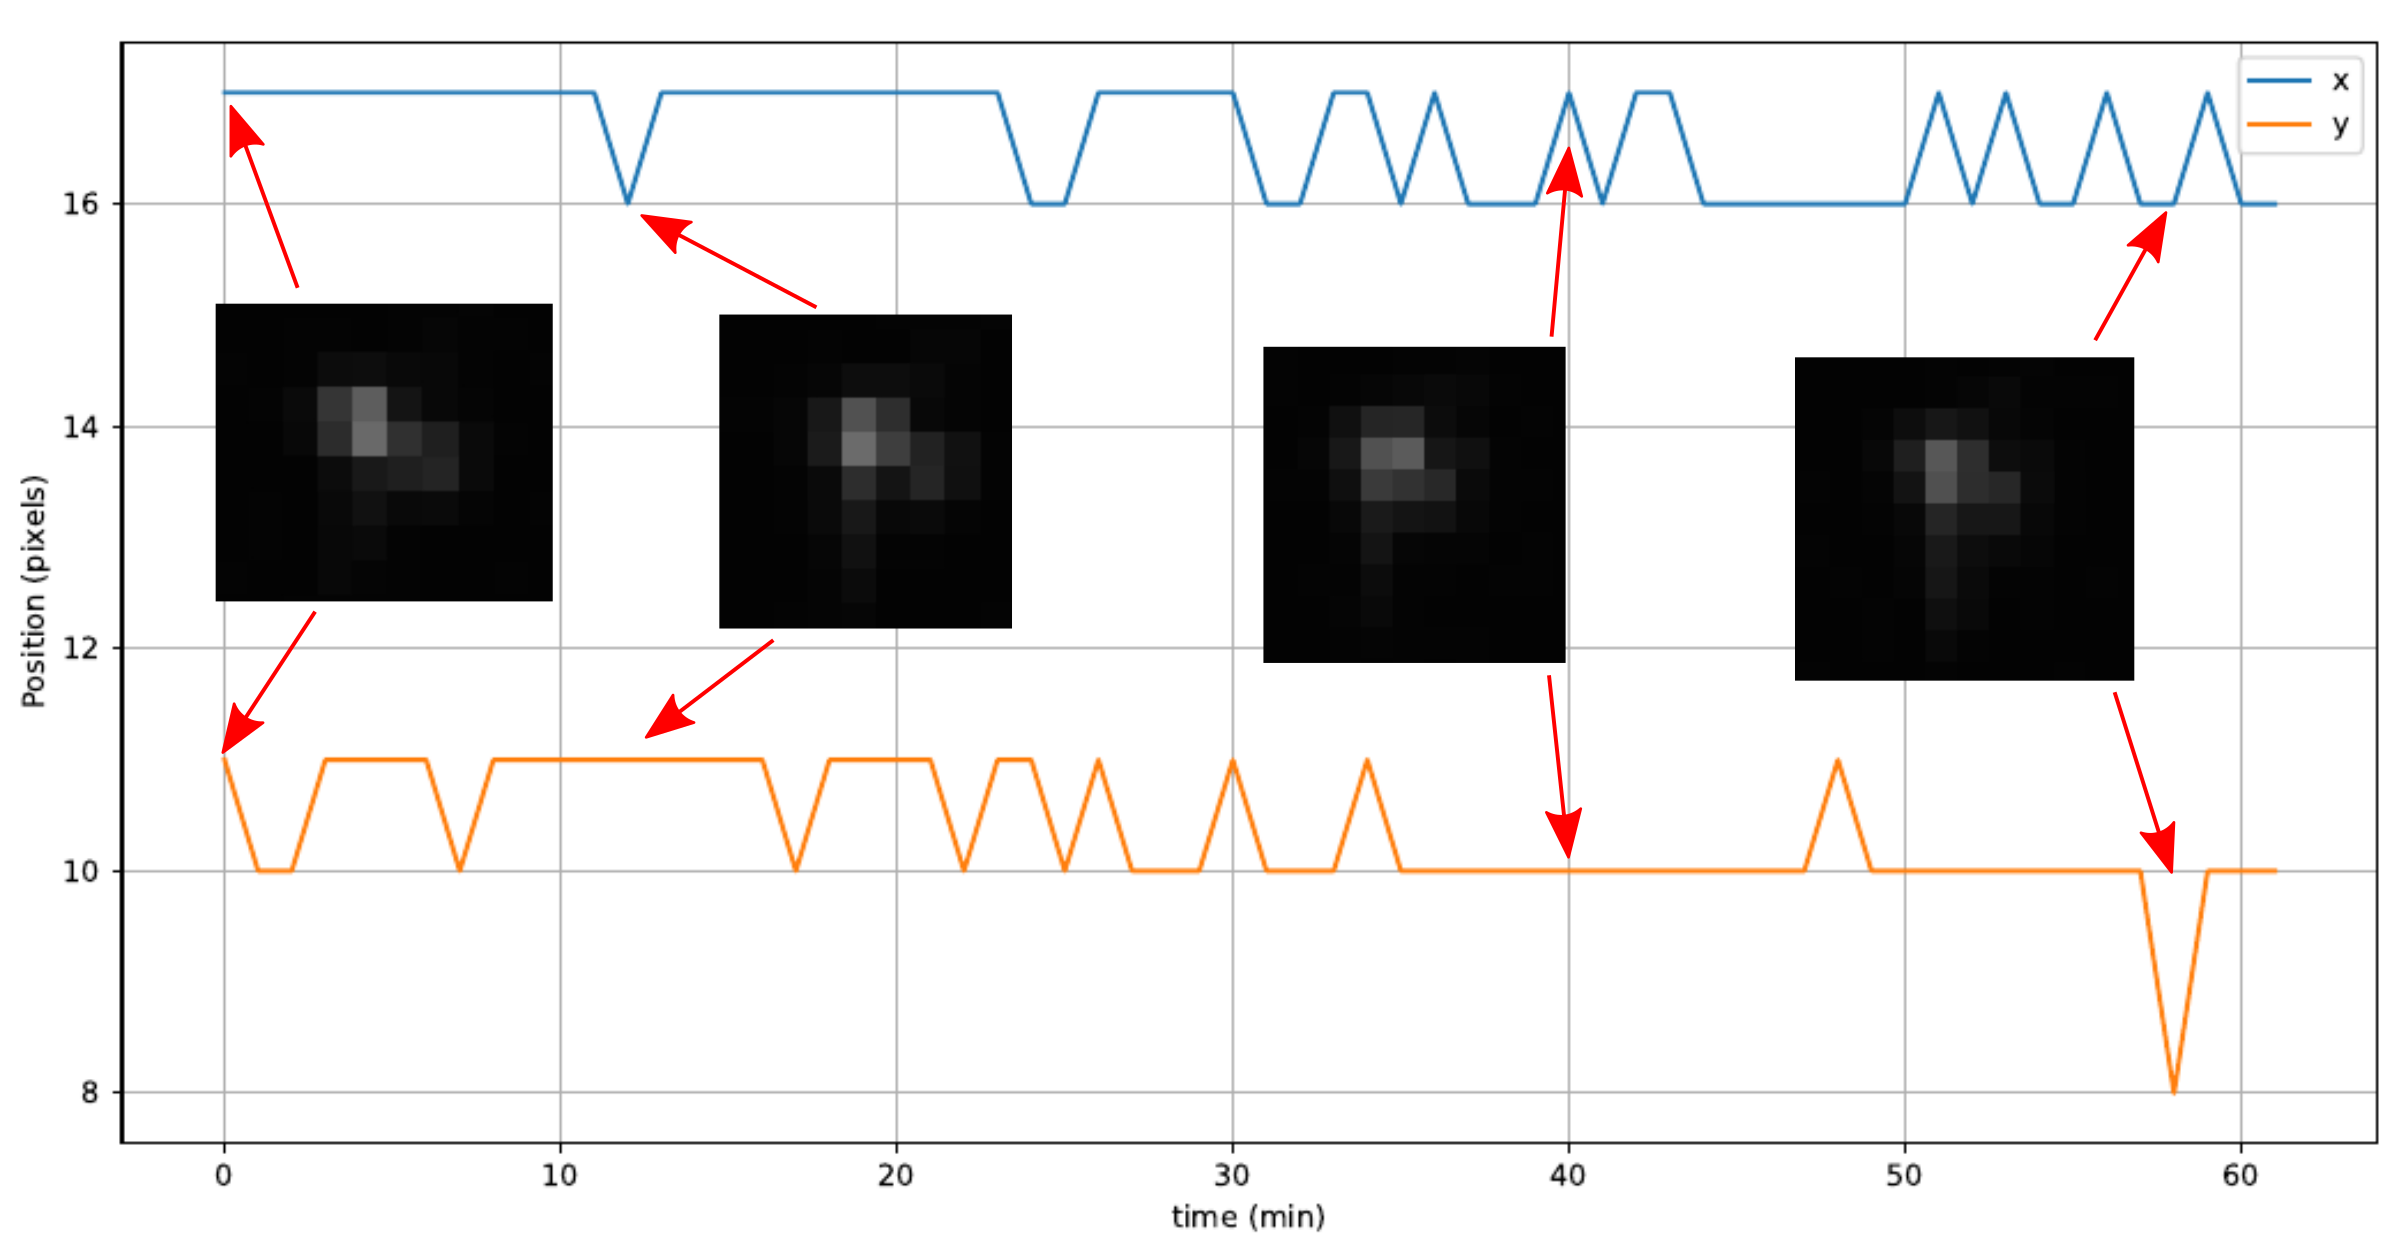
\includegraphics[width = .9\textwidth]{beampointing2}
\caption{Beam pointing stability at the focus position over a period of one hour. The 2 lines represent the horizontal $x$ and vertical $y$ position of the beam in unit of pixels. In the insets, some examples of raw data are given.}
\label{beampointing}
\end{figure}


\newpage
\section{Final installed system}
\label{sec:finalsetup}
After the tests presented in the previous sections, the setup was installed next to the ion chamber and focused on the ions as described in Section \ref{design4}. As there is no more physical access to the focus spot, more advanced quantum optics experiment have to be carried out in order to measure properties of the system, such as focus spot size and addressing error. The first experiment designed aims exactly at measuring these two quantities: a Ramsey experiment was performed on four loaded ions, from which the beam shape due to addressed AC Stark shifts on the ions could be measured.
The second experiment involves three ions and the goal was to generate photons via Raman process from one single ion leaving the states of the other two unaltered, demonstrating therefore the new possibility to emit single photons from individual ions in a string.

\subsection{Single qubit manipulation}
\label{sec:singlequbitmanipulation}
\begin{figure}[H]
\centering
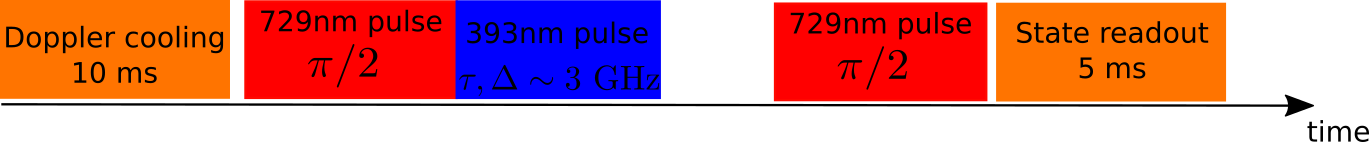
\includegraphics[width=\textwidth]{sequence}
\caption{Pulse sequence of the Ramsey experiment. The sequence is repeated for different AOD frequencies moving the 3 GHz detuned 393 nm beam across the ion string. From the ion excitations, the Rabi frequency of the 393 nm laser can be inferred. All operations are on all ions simultaneously, except the 393 nm pulse which is ideally addressed. The length $\tau$ was varying.}
\label{sequence}
\end{figure}
The goal of this experiment is to perform the Ramsey experiment discussed in Section \ref{sec:expqubit}. In summary, we want to sweep the 393 nm beam along the ions, the sequence in Figure \ref{sequence} is repeated for different AOD frequencies, and from the ion excitation we can infer the Rabi frequency of the 393 nm laser. Before the experiment, some preliminary measurements have to be taken, thus in this section we show first the following:
\begin{itemize}
\item Global Rabi flops with 729 nm, from this we can measure the $\pi/2$ pulse time and show individual ion readout with the camera.
\item Ramsey fringes without 393 nm, showing coherent control over the ion qubits.
\item 393 nm pulse length scan, to determine the length $\tau$ of the Raman pulse to achieve particular $\sigma_z$ rotations and furthermore to estimate the addressing error.
\end{itemize}
After these preliminary steps we performed the Ramsey experiment scanning the frequency of the AOD, as we scan, every single ion will produce a signal proportional to the Rabi frequency $\Omega$ that can be fitted to obtain the focus spot size.\\
These experiments were done with four ions loaded in the trap with endcap voltages of 714 V and 700V, for which numerical simulations yield a axial COM frequency of $\sim$767 kHz. The 393 nm laser was locked to the wavemeter and detuned by $\sim$3 GHz, ref. Section \ref{sec:expqubit}.\\

Global Rabi flops are showed in Figure \ref{rabiflops4}. Some point are missing in the plot due to a melting event of the ion crystal. The system took the data points while ions were melted, therefore they have been removed. Rabi flops are also damped due to residual thermal distribution, since we only perform Doppler cooling, ions are not in the ground state, but rather in a thermal state \cite{ross}. The $\pi/2$ time is extrapolated from the first flop as the time it takes for the ions to reach excitation probability $P_D = 0.5$, we estimated 4.2 $\mu$s. Errorbars on the excitation probability have been assigned according to the error on estimating the probability of a binomial distribution \cite{mle}
\begin{equation}
\label{errorequation}
\sigma = \sqrt{\frac{P_{D}(1-P_{D})}{N}},
\end{equation}
where $N = 50$ is the number of repetitions.
\begin{figure}
\centering
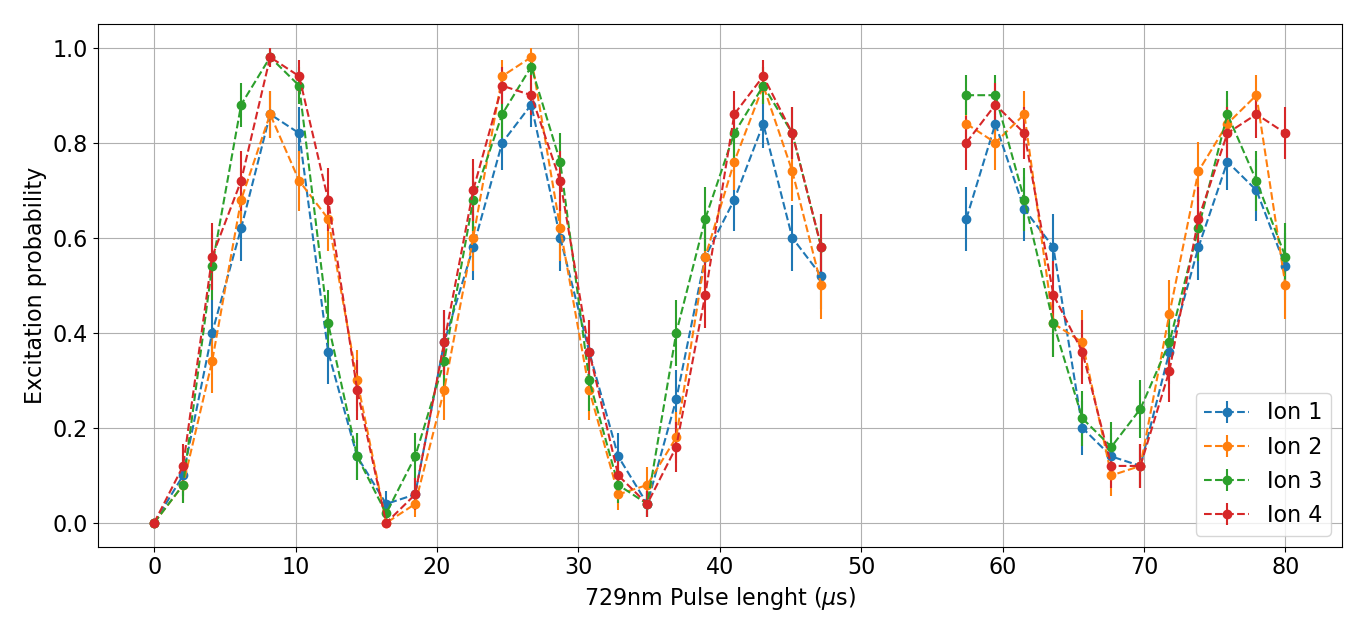
\includegraphics[width=\textwidth]{rabiflops2}
\caption{729 nm global Rabi flops on 4 ions measured with the camera. Errorbars on the excitation probability have been assigned according to the error on estimating the probability of a binomial distribution. Some points were removed due to a melting event.}
\label{rabiflops4}
\end{figure}
Ramsey fringes without the 393 nm pulse are presented in Figure \ref{ramseyfringes}, the $\pi/2$ time was set to 4.2 $\mu$s. The phase $\phi$ between the two pulses was scanned, and afterwards it was set to $\phi = \pi/2$ for the rest of the experiment.
\begin{figure}[H]
\centering
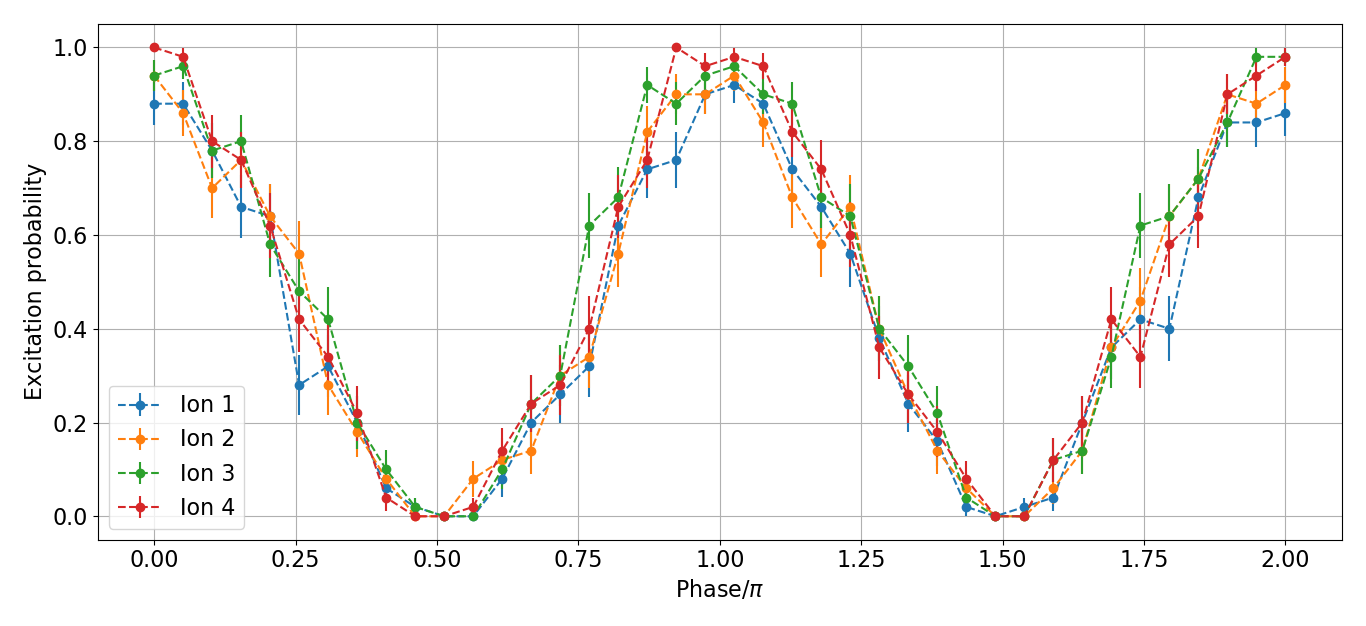
\includegraphics[width=\textwidth]{ramseyfringes}
\caption{Ramsey fringes for 4 ions without 393 nm. A $\cos^2(\phi)$ behavior can be noticed showing coherent control of the ion states.}
\label{ramseyfringes}
\end{figure}
The 393 nm pulse lenght $\tau$ was scanned inside the Ramsey experiment, the flops are showed in Figure \ref{ACscan}. For the next experiment, to get the beam profile across the ion string, we chose $\tau$ of 25 $\mu$s, so that the ion is not fully flipped. It was roughly checked that $\tau$ is the same for every ion.
\begin{figure}[H]
\centering
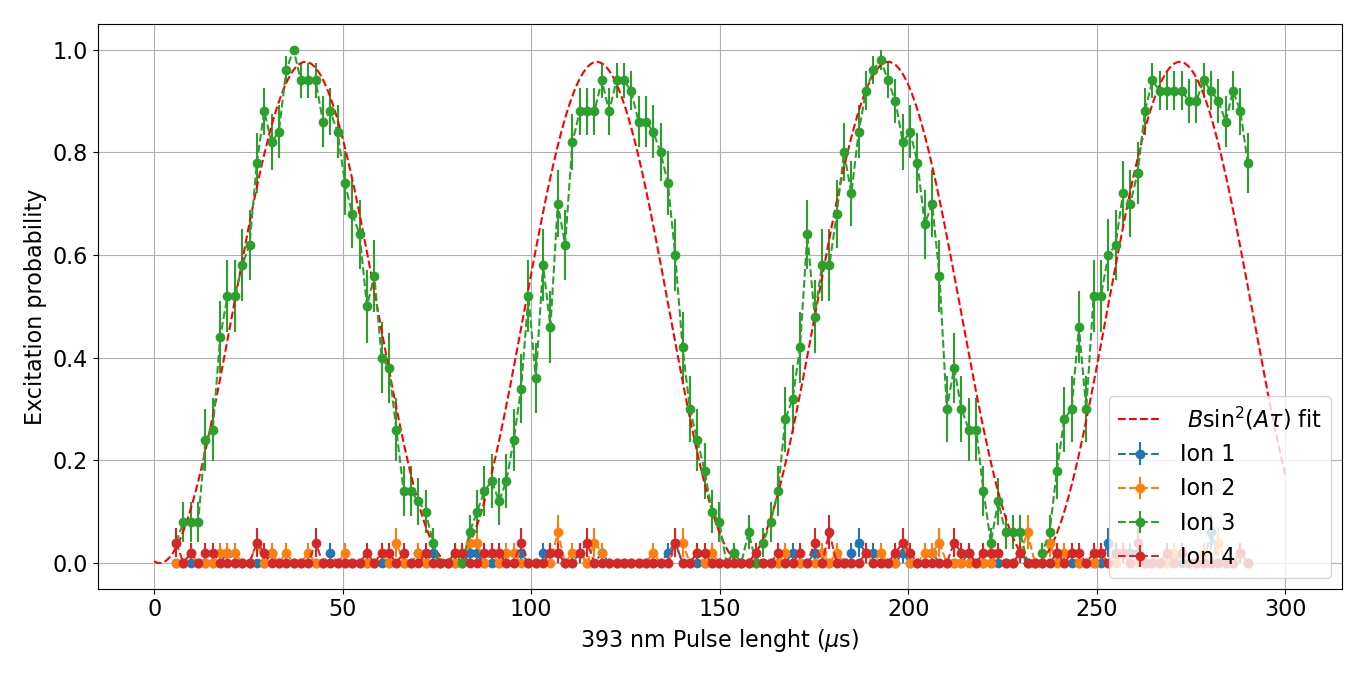
\includegraphics[width=\textwidth]{ac_stark_fit}
\caption{393 nm AC Stark flops. The pulse length $\tau$ of the 393 nm laser is scanned while shining over one singe ion. The red curve is a fit of $B\sin^2(A\tau)$, where $A$ is proportional to the Rabi frequency of the laser focused on the third ion.}
\label{ACscan}
\end{figure}
Finally, the AOD frequency is scanned, during this scan the beam is moved from ion to ion and the excitation probability of all ions is measured, this is then translated to Rabi frequency with equation \eqref{eq:ptointensity}. The result after further post analysis can be seen in Figure \ref{AODscan}. Specifically, the square of the Rabi frequency, determined from the probability $P_D$, gives the laser intensity of the beam, errors are propagated accordingly.
\begin{figure}
\centering
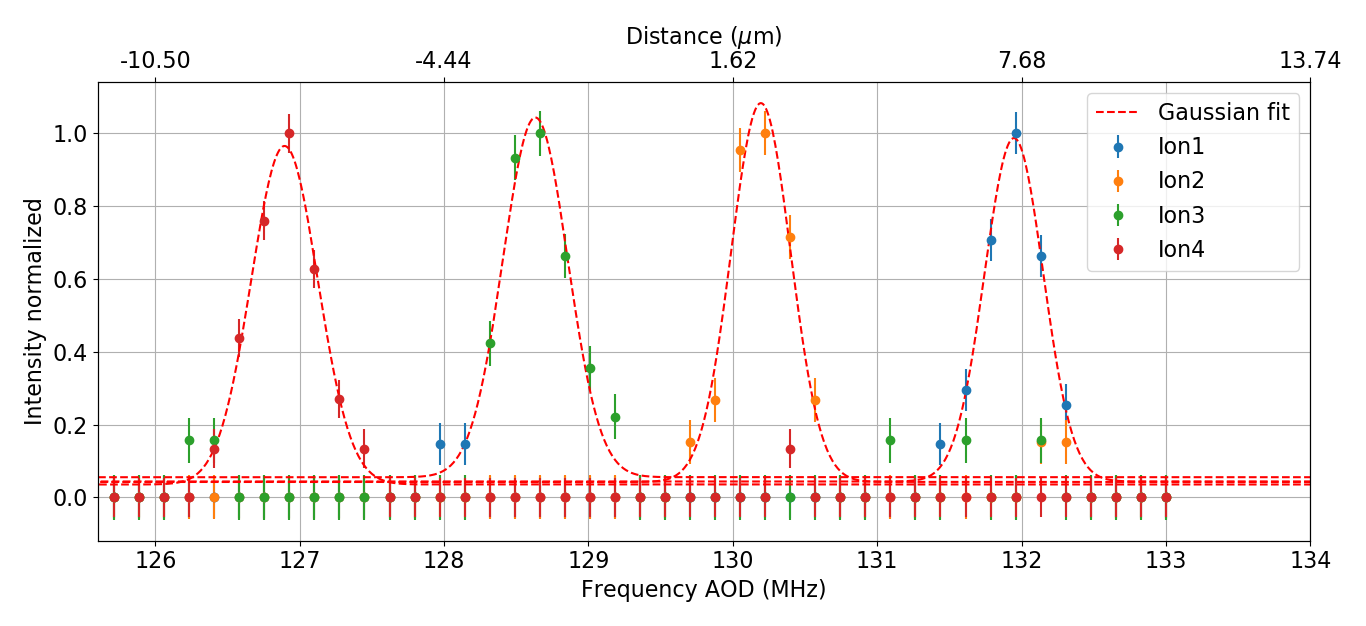
\includegraphics[width=\textwidth]{img/AODScan}
\caption{AOD scanning of four ions via Ramsey interferometry. The normalized intensity comes from the Rabi frequency calculated from the excitation probability $P_D$ using formula \eqref{eq:ptointensity}. The upper micrometer scale is calibrate by comparing the center of the Gaussian fit with the numerically calculated ion positions.}
\label{AODscan}
\end{figure}
To calibrate the beam position scale in micrometers, the axial COM mode (767 kHz) of the trap is measured by performing 729 nm spectroscopy on the carrier and motional sideband. Ions positions can be then numerically calculated (cfr. Section \ref{ionstrings}). AOD frequencies corresponding to the maxima in Figure \ref{AODscan} are attributed to the ion positions, and corresponding frequency shifts to distances. By comparison, we found a conversion factor of $3.03\,\mu\text{m}/\text{MHz}$.
The four peaks have been fitted with a Gaussian function to obtain the waist of the beam when focused on the different ions. The waists yielded by the fits are from right to left $\omega_1 = 1.23\pm 0.20\,\mu$m, $\omega_2 = 1.25\pm 0.19\,\mu$m, $ \omega_3 = 1.35\pm 0.22\,\mu$m, $\omega_4 = 1.39\pm 0.20\,\mu$m.\\
The Figure \ref{ACscan} allows the addressing error, when aiming at ion 3, to be determined. In this measurement, the addressing beam was focused on one ion and the Raman length $\tau$ is scanned. This increases the interaction time of the laser with the ions, and if the interaction is long enough even the tail of a Gaussian can induce some excitation on the ions on the side of the one being addressed. In the scan displayed, the pulse reached 300 $\mu$s and there is no statistically significant excitation on any ion apart from the one flopping. Others scans went up to 500 $\mu$s, and still no visual excitation is present. While this means that no quantitative number can be determined for the addressing error, an upper bound can still be given. A sinusoidal fit $B\sin^2(A\tau)$ has been done on the data, it is not perfect probably due to intensity fluctuations of the lasers, or magnetic field fluctuations. Nonetheless, from the fit we can determine the Rabi frequency on the third ion as $\Omega_3 = \sqrt{4\Delta \cdot A} = 22\,\text{MHz}$, see equation \eqref{stupidequation}. Assuming in the worst case scenario that an excitation $P_D>0.05$ on the second ion appears right after 500 $\mu$s, i.e. the Rabi frequency of the non-addressed ion is $2$ MHz, the addressing error should be at most $\Omega_2^2/\Omega_3^2< 10^{-2}$.\\
During this experiment we scanned the AOD twice in a interval of 30 minutes to measure the stability of the system. In Figure \ref{fig:stability} the peak on the third ion has been overlapped between the two scans. A fit gives the central frequencies of the two peaks, and their difference determines the stability over a period of 30 minutes, we estimated a stability of $0.20\pm 0.07\,\mu$m/h.\\
To conclude this section, we remark that the 393 nm pulse acts as a single qubit gate on individual ions. The Ramsey experiment carried out by scanning the AOD frequency demonstrated the ability of the system to manipulate single qubits as it includes a single qubit rotation $\sigma_z$ first introduced in section \ref{sec:quantumoperations}. The Ramsey experiment therefore fulfills a goal of this thesis, however the gate quality of $\sigma_z$ needs to be studied more carefully in the future.
\begin{figure}
\centering
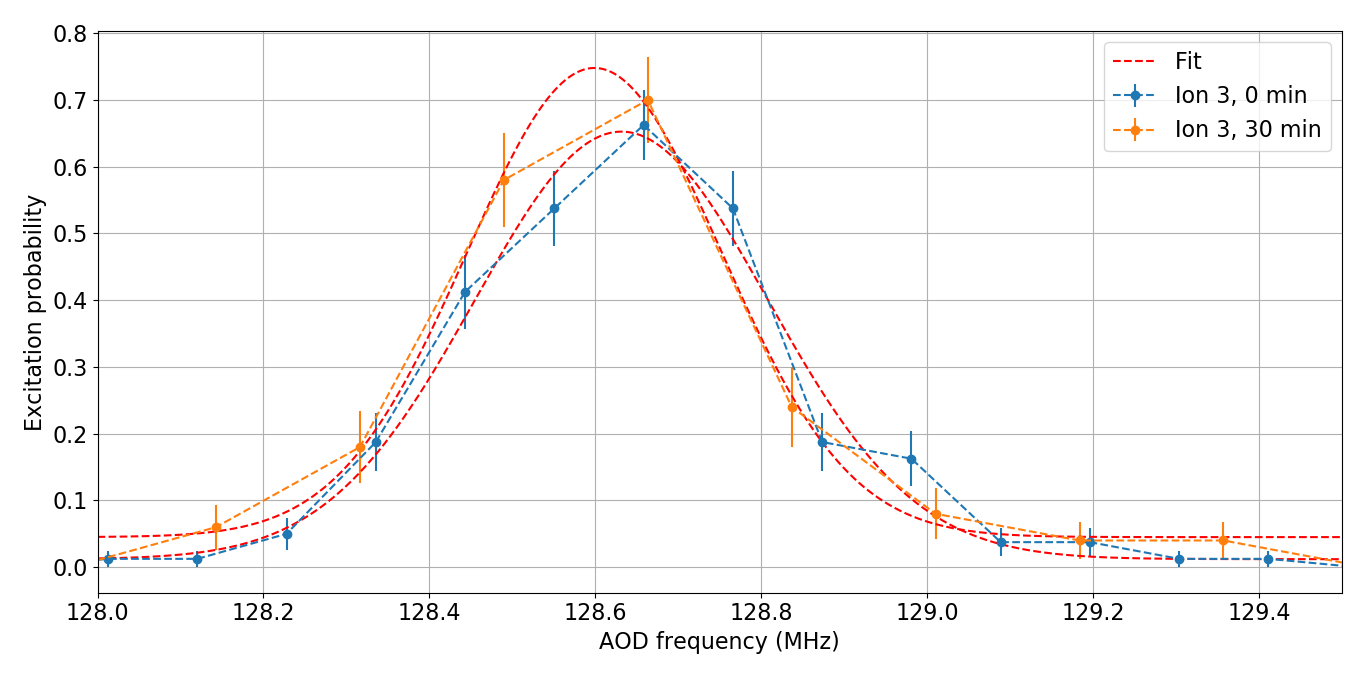
\includegraphics[width=\textwidth]{stability}
\caption{AOD scanning on one single ion repeated after 30 minutes to measure stability as difference of the center of the two peaks: $0.20\pm 0.07\,\mu$m/h. Processing of the data has been done as in Figure \ref{AODscan}.}
\label{fig:stability}
\end{figure}
\subsection{Photon production}
\label{exp:photons}
The second goal is to generate single photons from individual ions in a chain. Photons are produced by a pulse of 393 nm light focused on the central ion of three via the cavity-mediated Raman process described in Section \ref{sec:expphoton}. The length of the Raman pulse is scanned and the integrated photon detection probability is recorded, measured leaving the cavity. The generated photon is emitted into the cavity, transmitted through the mirror of the cavity, coupled into an optical fiber, and passes through waveplates and a PBS before reaching a superconducting nanowire single-photon detector (SNSPD)\footnote{Scontel SNSPD model FCOPRS-CCR, 854 nm detectors: $\sim 87$\% efficiency, $\sim 0.5$ dark counts per second.}. In contrast to the previous experiment, the precise (to the kHz level) frequency of the Raman laser is key to generate cavity photons. Here the laser is locked to an external cavity (linewidth $\sim$100 Hz Ref. \cite{helene}). The existing AOM network was established to leave the Raman laser 400 MHz detuned from the S-P transition. To account for the additional 127 MHz detuning of the AOD, we shifted the frequency of two AOMs in the 393 nm setup (see Section \ref{sec:393setup}).\\
%The experiment was carried out in a single day at the end of the time available for my master work.
We loaded three ions in the trap with a measured axial COM frequency of $\sim 820$ kHz, which means ion separations of 5.4 $\mu$m. We locked the 393 nm laser to the cavity and scanned the Raman transition with the double pass AOM 1 (ref. Figure \ref{scheme393}). The transition chosen is $\ket{S_{1/2},-\frac{1}{2}}\to \ket{D_{5/2},-\frac{3}{2}}$, see details in Section \ref{sec:expphoton}. The cavity position along the axis was optimized by maximizing overall 854 nm photon count rate when driving the Raman process with the addressed beam aligned to the central ion, and simultaneously repumping the 854 nm transition. Assuming that the central ion is at a maximum of the cavity field and that the cavity-trap angle is $4.6^\circ$, we calculated that the two outer ions are at 82 \% of the cavity maximum.
In the experiment we included an initial stage of Doppler cooling and a final stage of state detection with the camera. Furthermore, the 806 nm cavity locking light was switched off during the photon generation process, in this time the cavity maintained its position with a sample and hold. For each Raman pulse length, the experiment is repeated $N=200$ times to get an estimate for the average photon probability and the ion excitation probability ($P_D$ the probability to find the ion in the D5/2 manifold). Errorbars on the excitation probability are calculated as the previous section (equation \eqref{errorequation}), while for the photon probability the error is modelled by Poissonian statistics \cite{quantumoptics}
\begin{equation}
\sigma_{ph} = \frac{\sqrt{N_{click}}}{N},
\end{equation}
where $N_{click}$ is the number of times a photon has been detected with respect to the total $N$ repetitions. \\
The experiment consisted of scanning the Raman pulse length, and for each length, the photon detection probability and the ion excitation probability $P_D$ have been measured. In Figure \ref{probphoton}, the photon detection probability is plotted. From the resonant transition polarization selection rules, we expect a $\pi$ polarized photon being emitted. As the cavity is perpendicular to the magnetic field, the photon is projected into linear polarization and rotated such that it goes to one output port of the PBS. Consistently with the expectations, we can see that we measured mostly vertical polarized photons. The photons are not perfectly polarized which could be due to imperfections of the polarization analysis, e.g. misaligned waveplates.\\
The excitation probability $P_D$ is plotted in Figure \ref{probion}. In this figure, we can see that only the addressed ion is being excited to the $\text{D}_{5/2}$ state, while the others show no excitation at all. $P_D$ does not reach 1, perfect population transfer is not achieved due to non-zero spontaneous emission from the $\text{P}_{3/2}$ state to the $\text{D}_{3/2}$ state, or to the $\ket{S_{1/2},+\frac{1}{2}}$ state. In fact, as calculated is section \ref{sec:ramanprocess}, the effective spontaneous emission is still around one half of the effective Rabi frequency. Unfortunately, we were not able to simulate theoretical curves for both of the plots, as the experiment was carried out in one day at the end of the time available for my master work. As such, no careful optimization was done on the polarization of the driving addressing beam, which means that the parameters are not well known enough do a theoretical model. We remind that the two outer ions are still coupled to the cavity to some extent, i.e. they are in condition to get excited and emit photons. In fact, we also observed photon generations when addressing outer ions. Characterization of multiple ion coupling is however beyond this work. \\
In conclusion, we observed the addressed ion getting excited to the $\text{D}_{5/2}$ state and simultaneously detected vertical polarized photons. Therefore, these data are consisted with only the middle ion emitting photons.

\begin{figure}[H]
\centering
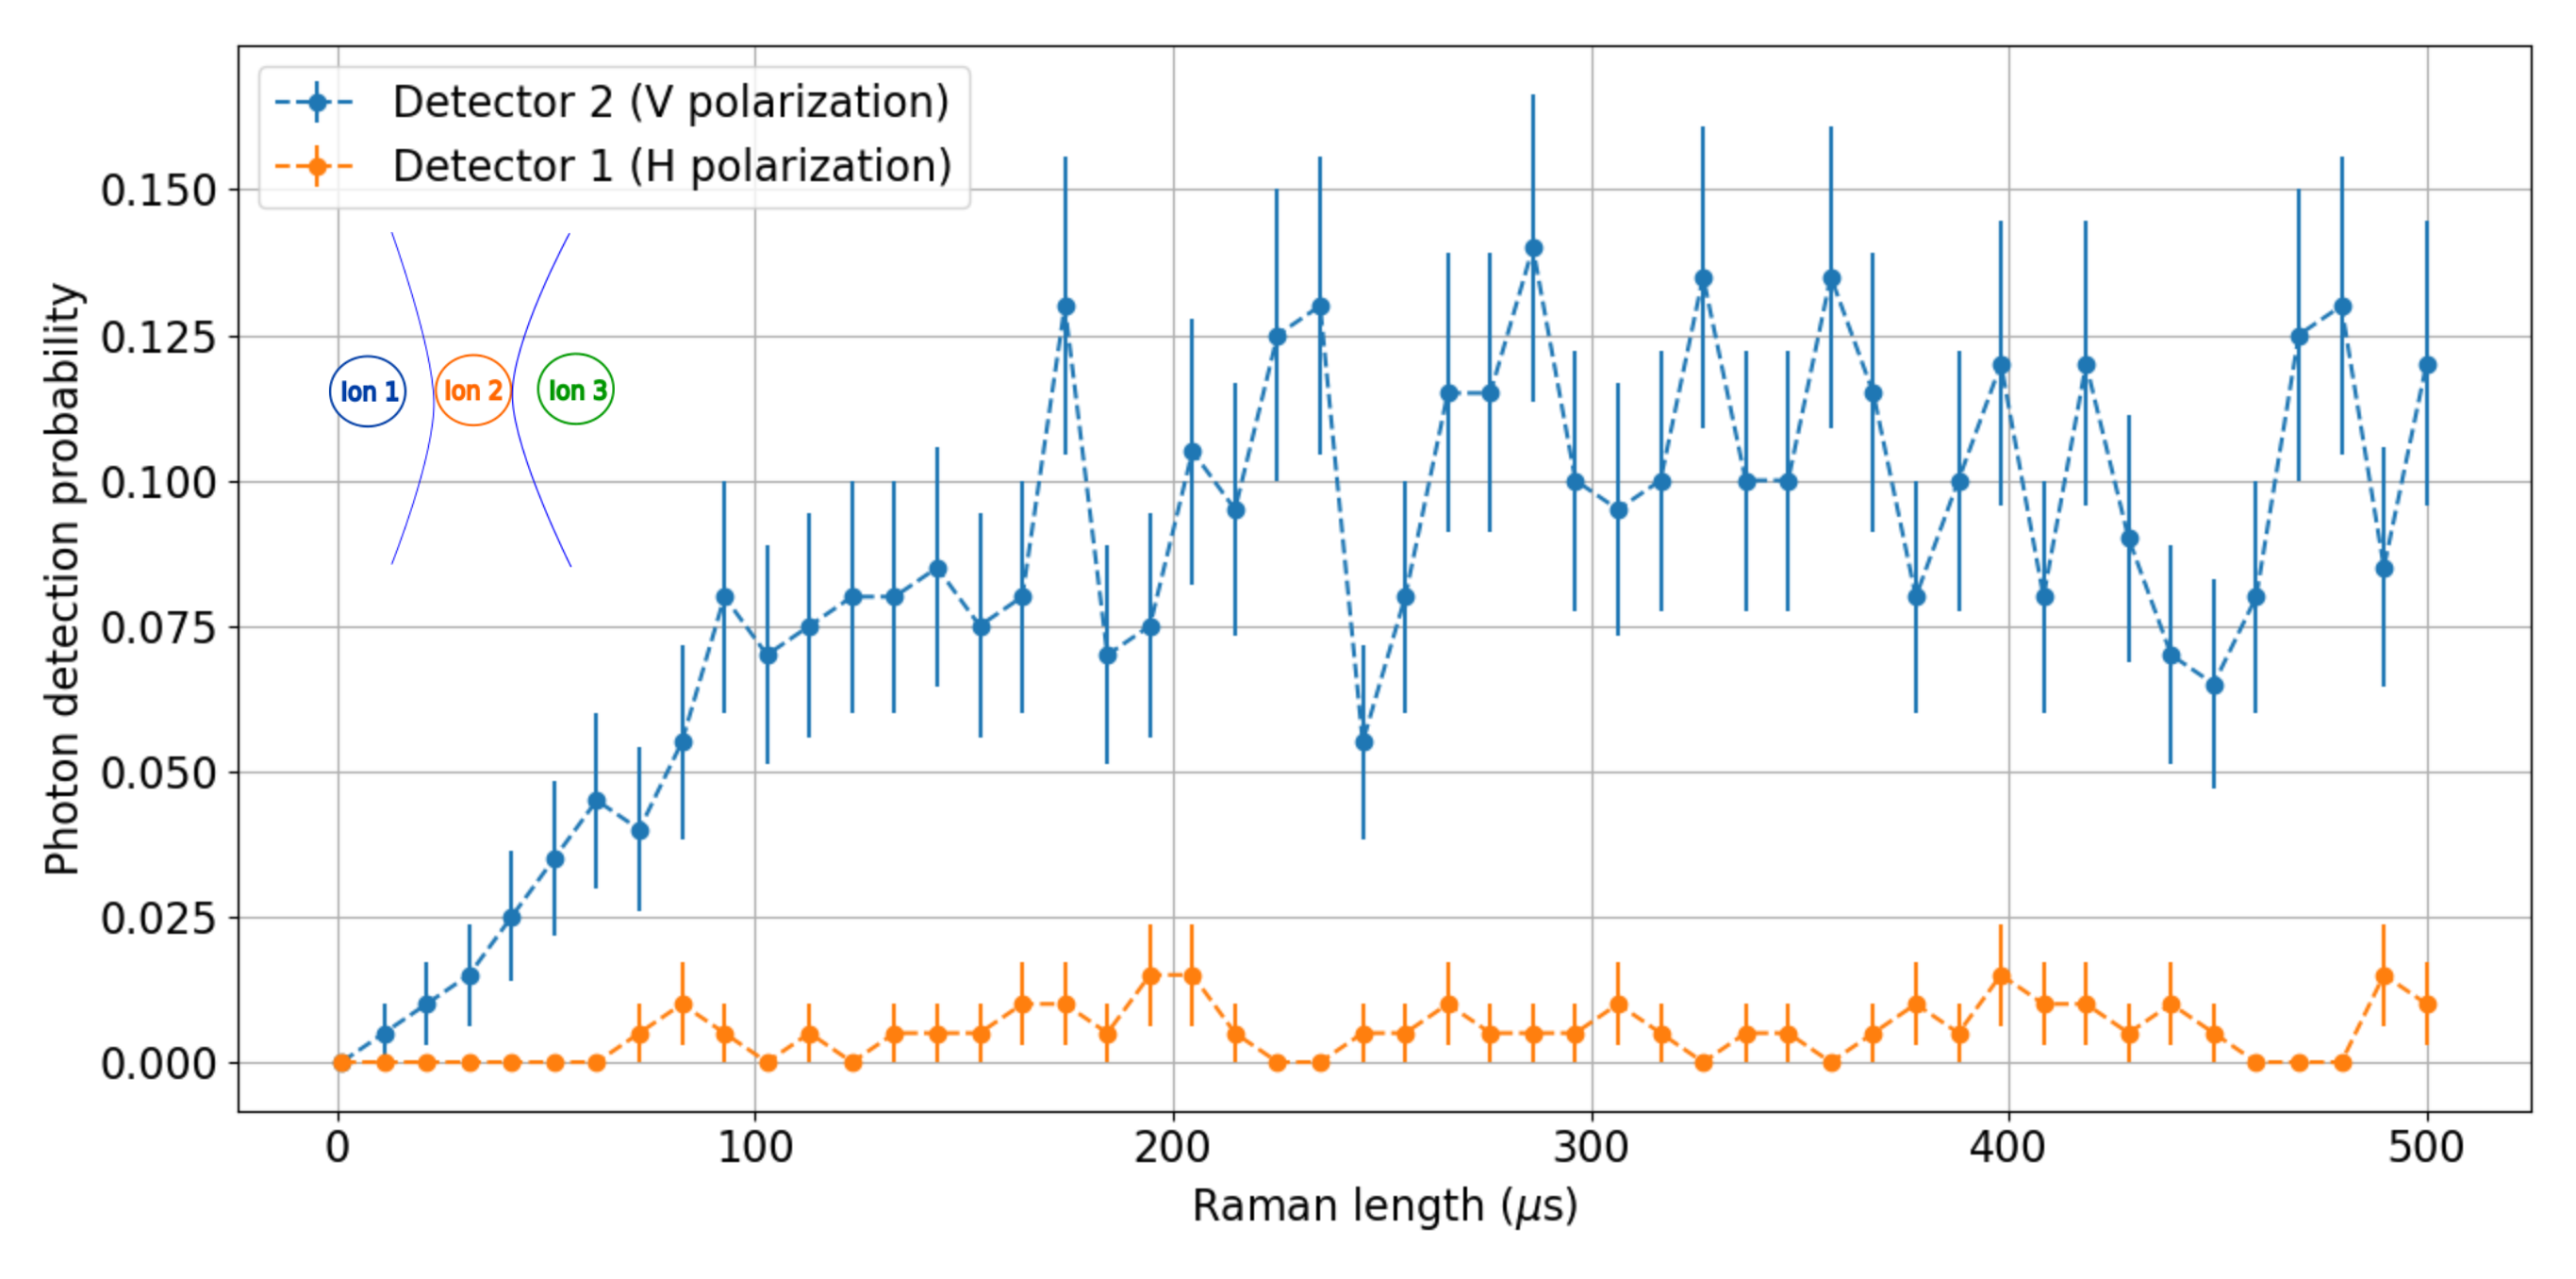
\includegraphics[width=\textwidth]{img/photonefficency_witherror3}
\caption{Measured cavity photons as a function of addressed Raman laser pulse length. The two detectors measure the Horizontal (1) and Vertical (2) photons emitted by the ion, in Figure \ref{probion} excitations of the ions during the process are plotted. Under the legend a diagram sketching the situation where only the middle ion is addressed.}
\label{probphoton}
\end{figure}
\begin{figure}[H]
\centering
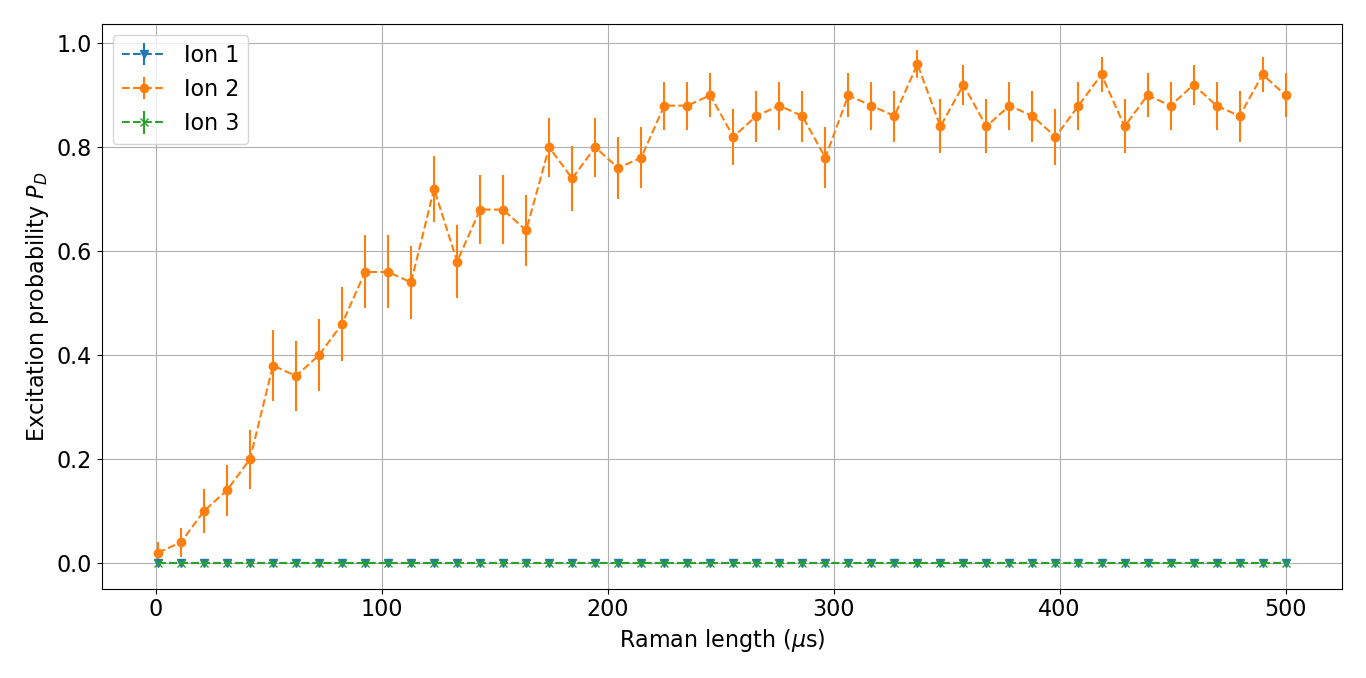
\includegraphics[width=\textwidth]{img/ramanlength_witherrors2}
\caption{Qubit state of the ions $P_D$ as a function of addressed Raman laser pulse length. In Figure \ref{probphoton} photon detection probability during the same process is plotted.}
\label{probion}
\end{figure}
% \section{Final properties summary}
% This section contains a summary of the different properties of the setup, everything can be found in the figure below.
% \begin{figure}[H]
% \centering
% 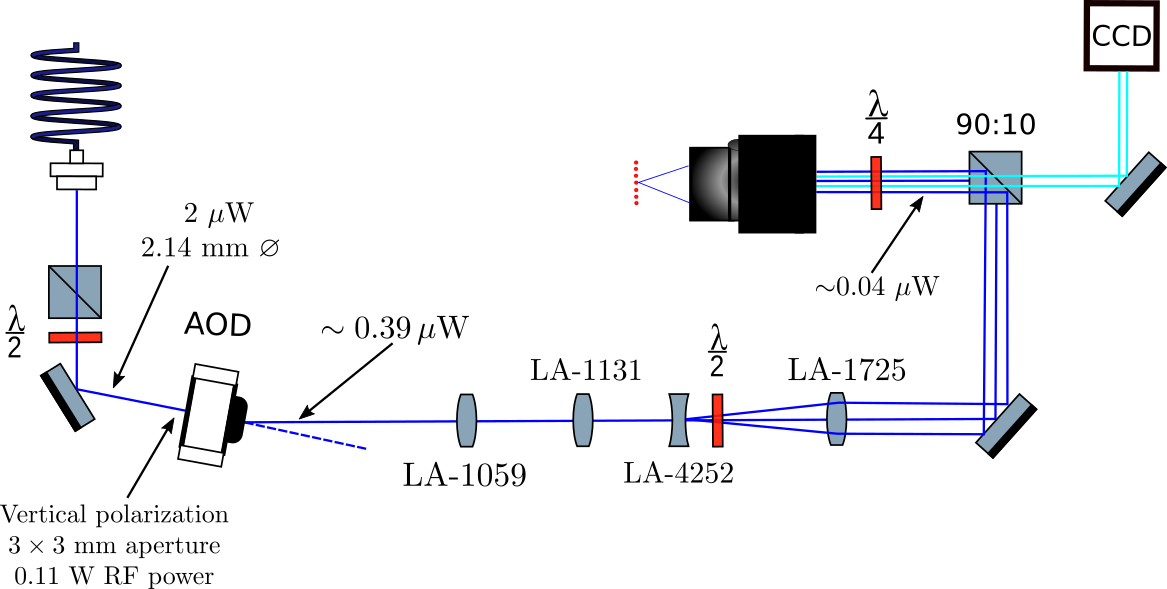
\includegraphics[width = \textwidth]{recap}
% \caption{Properties summary of the setup.}
% \end{figure}


%Conclusion
% !TEX root = main.tex

\chapter{Conclusions and outlook}
In this thesis works, an optical setup for single ion focusing of 393nm laser has been designed and built.

The setup was intended to be used for single photon generations and single qubit manipulations. Both of the purposes has been filled: the photon generation was demonstrated in
experiment in section \ref{exp:photons}, here a string of three ions was loaded into the trap and the focused laser aligned with the central one. A laser pulse triggered the photon generation exclusively from the intended ion as we can see from the excitation probability. The photon detection probability was low $<15\%$, and can definitely be further improved. Qubit manipulation was carried out in the Ramsey inteferometer experiment, here we measured the AC stark shift caused by the 393nm light by imprinting a phase on the qubit encoded in the 729nm transition. State readout of the qubit showed the different final state for different phases. Moreover, with this experiment the waist of beam was measured to be $1.2-1.3\,\mu$m and the addressing error to have an uppperbound of $10^{-3}$.

The setup can still be optimized, during the experiments, polarization was not set correctly even if the system has the capabilities. Permanent magnets are still mounted parallel to the previous Raman laser, they have to be moved in the new direction. The next natural step is the generation of photons from different ions which requires all ions to be coupled to the cavity vacuum standing wave, a non trivial problem. Entanglement can also be produced between a single ion and a photon, once more stabilization improvement on the setup are done.


This project has several future development, on the quantum network side, this work represents an improved interface between network and quantum computer, transmission bandwidth has drastically increased, dedicated qubits for networking, storing, and computation can now be created and manipulated. It also opens up to the possibility to create multi-ion-multi-photon states with applications in quantum metrology.


\newpage
%\renewcommand\refname{References} % name for the reference list

\addcontentsline{toc}{section}{References} % to change the name of the references in the TOC
\bibliographystyle{unsrt}
\bibliography{References} % adds the references to the document


\newpage
\renewcommand{\appendixpagename}{Appendix} % Heading of appendix
\renewcommand{\appendixtocname}{Appendix} % name of appendix in TOC
%\appendixpage
\addappheadtotoc

\begin{appendices}
\chapter{AOD datasheet}
\label{sec:aoddata}
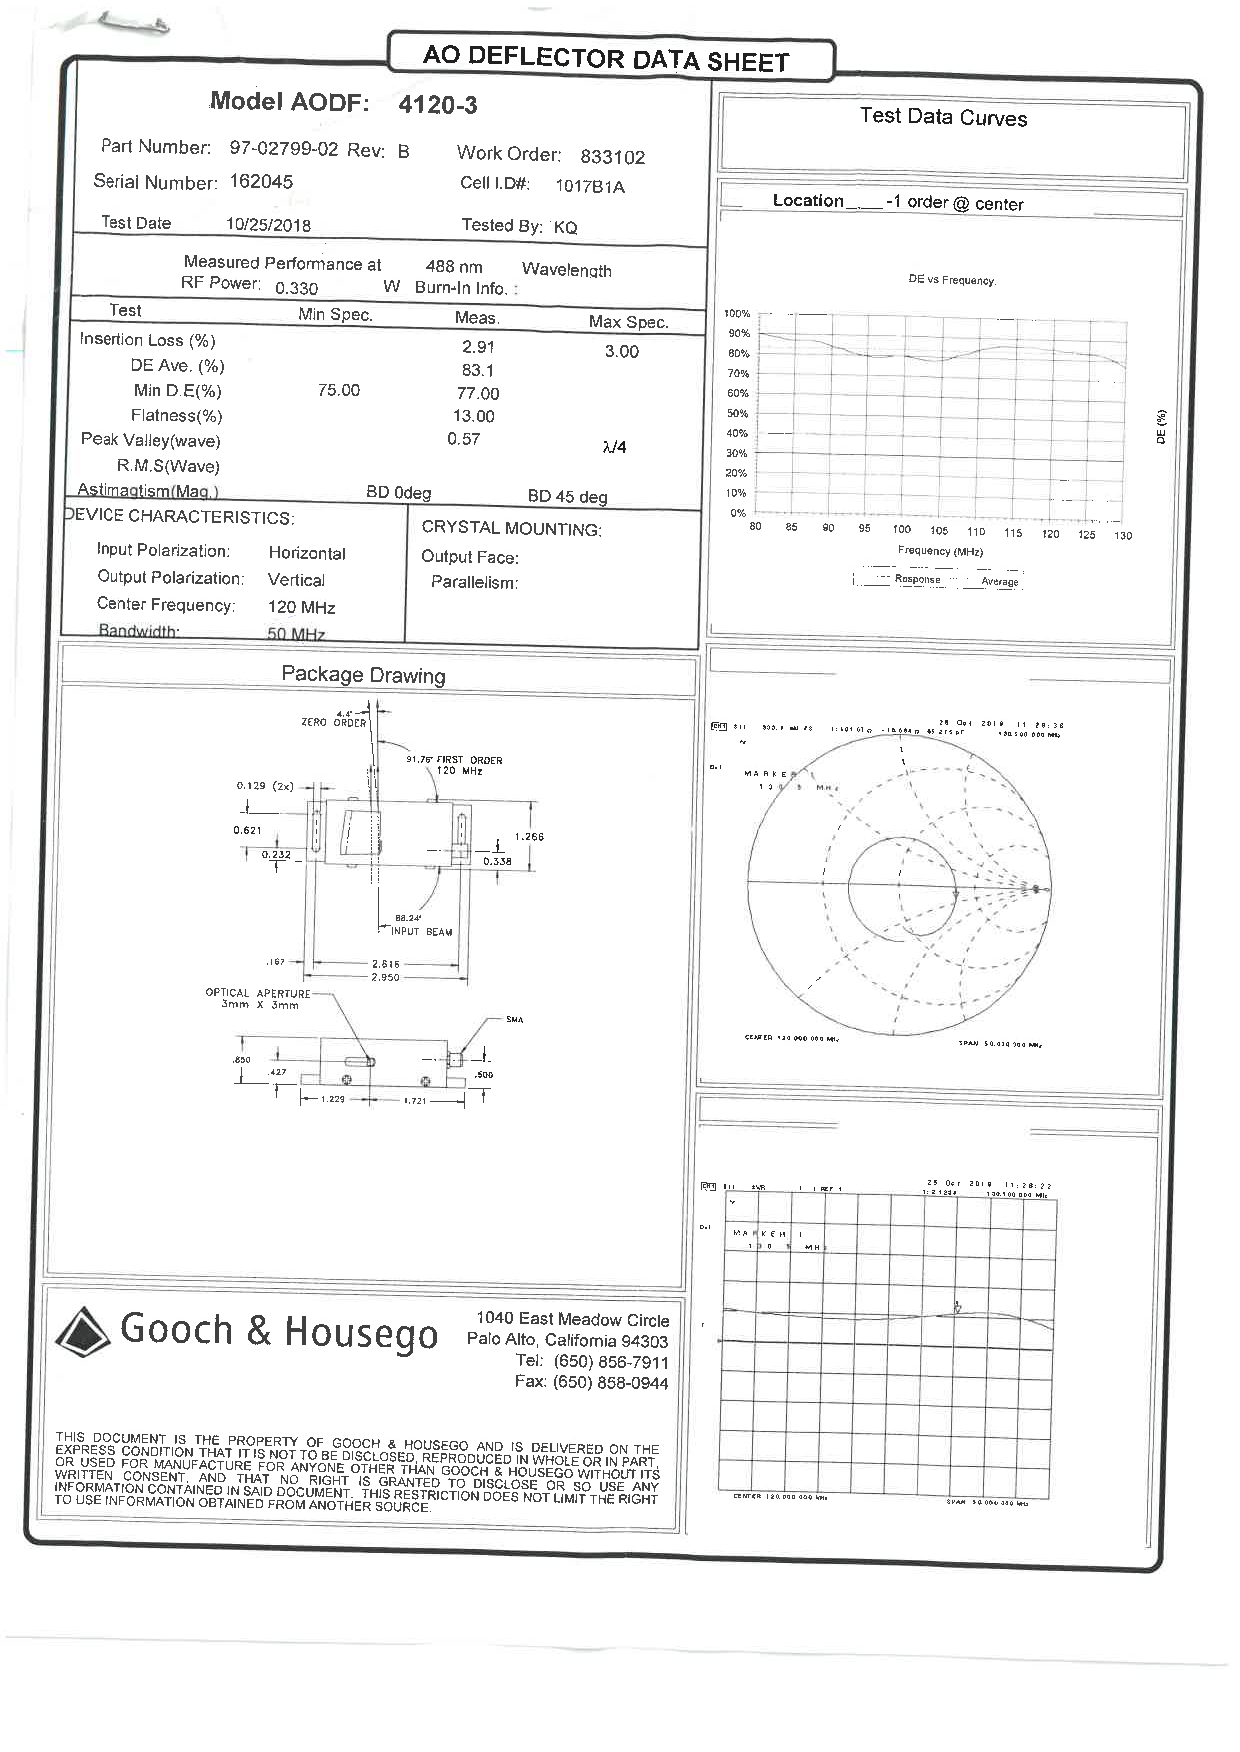
\includegraphics[scale=0.7]{SKM_C36819012815280}
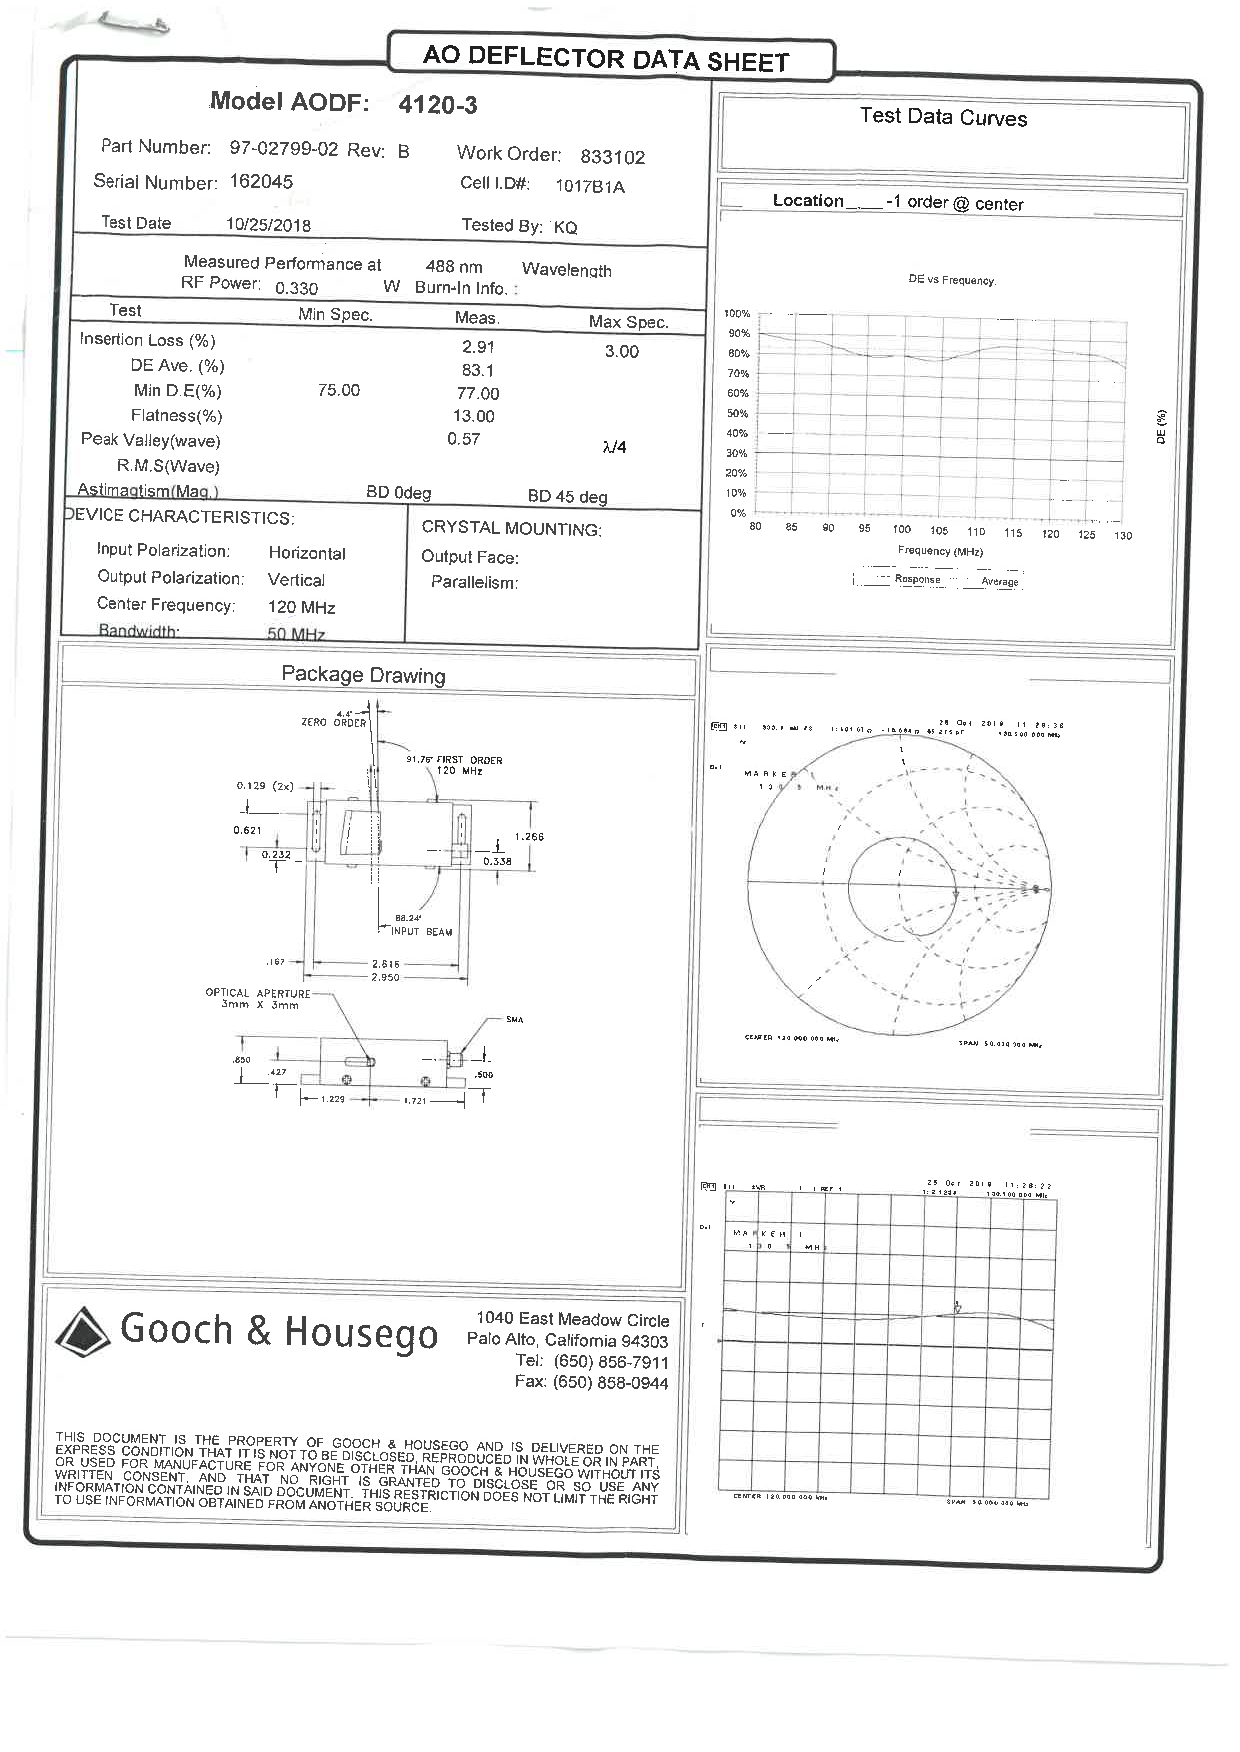
\includepdf[page={2-}]{SKM_C36819012815280}
\chapter{Polarization characterization}
\label{app:polarization}
Here we report the figures for the polarization characterization of section \ref{sec:polarization}. Every figure contains a fit of a sine function $A\sin(\omega x +\phi)$, where $x$ is the angle of the corresponding waveplate. The fit are used to determine the maxima and minima of the curves which indicates the closest point to the desired polarization, see table \ref{polarizationstable} for results.
\begin{figure}[H]
\centering
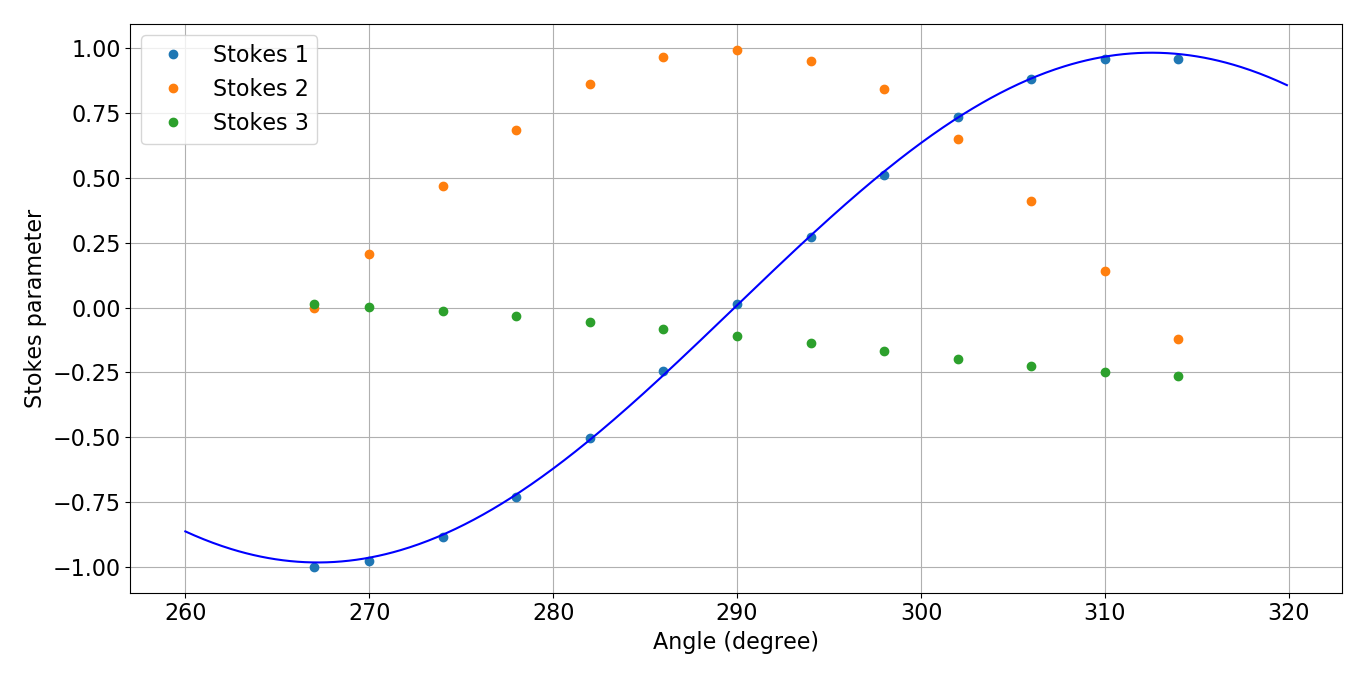
\includegraphics[width = \textwidth]{pol3}
\caption{Polarization after the $\lambda/2$ WP (see figure \ref{addressingsetup}) as a function of the $\lambda/2$ WP B angle. Blue line is a sine function fit: $A = 0.983 \pm 0.007, \pi/\omega = 45.3 \pm 0.6^\circ$.}
\label{pol1}
\end{figure}
\begin{figure}[H]
\centering
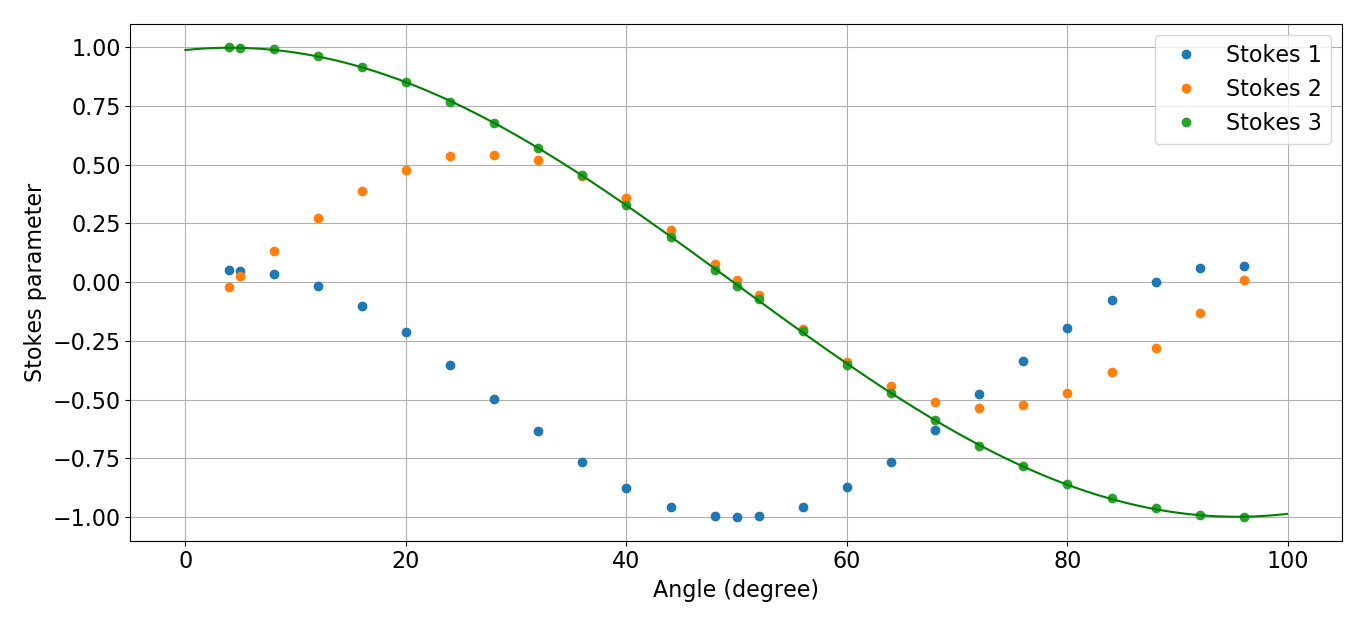
\includegraphics[width = \textwidth]{pol1}
\caption{Polarization after the objective at the focus spot as a function of the $\lambda/4$ angle with $\lambda/2$ WP B set to horizontal ($267^\circ$). Green line is a sine function fit: $A = 0.998\pm 0.02, \pi/\omega = 91.3\pm0.3^\circ$.}
\label{pol1}
\end{figure}
\begin{figure}[H]
\centering
\includegraphics[width = \textwidth]{pol2}
\caption{Polarization after the objective at the focus spot as a function of the $\lambda/4$ angle with $\lambda/2$ WP B set to vertical ($314^\circ$). Green line is a sine function fit: $A = 0.982 \pm 0.003,\pi/\omega = 90.0 \pm 0.5^\circ$}
\label{pol2}
\end{figure}
\end{appendices}

\end{document}
